% **************************************************************************************************************
% A Classic Thesis Style
% An Homage to The Elements of Typographic Style
%
% Copyright (C) 2015 André Miede http://www.miede.de
%
% If you like the style then I would appreciate a postcard. My address 
% can be found in the file ClassicThesis.pdf. A collection of the 
% postcards I received so far is available online at 
% http://postcards.miede.de
%
% License:
% This program is free software; you can redistribute it and/or modify
% it under the terms of the GNU General Public License as published by
% the Free Software Foundation; either version 2 of the License, or
% (at your option) any later version.
%
% This program is distributed in the hope that it will be useful,
% but WITHOUT ANY WARRANTY; without even the implied warranty of
% MERCHANTABILITY or FITNESS FOR A PARTICULAR PURPOSE.  See the
% GNU General Public License for more details.
%
% You should have received a copy of the GNU General Public License
% along with this program; see the file COPYING.  If not, write to
% the Free Software Foundation, Inc., 59 Temple Place - Suite 330,
% Boston, MA 02111-1307, USA.
%
% **************************************************************************************************************
\RequirePackage{fix-cm} % fix some latex issues see: http://texdoc.net/texmf-dist/doc/latex/base/fixltx2e.pdf
\documentclass[ twoside,openright,titlepage,numbers=noenddot,headinclude,%1headlines,% letterpaper a4paper
                footinclude=true,cleardoublepage=empty,abstractoff, % <--- obsolete, remove (todo)
                BCOR=5mm,paper=a4,fontsize=11pt,%11pt,a4paper,%
                italian,american,%
                ]{scrreprt}

%********************************************************************
% Note: Make all your adjustments in here
%*******************************************************
% ****************************************************************************************************
% classicthesis-config.tex 
% formerly known as loadpackages.sty, classicthesis-ldpkg.sty, and classicthesis-preamble.sty 
% Use it at the beginning of your ClassicThesis.tex, or as a LaTeX Preamble 
% in your ClassicThesis.{tex,lyx} with % ****************************************************************************************************
% classicthesis-config.tex 
% formerly known as loadpackages.sty, classicthesis-ldpkg.sty, and classicthesis-preamble.sty 
% Use it at the beginning of your ClassicThesis.tex, or as a LaTeX Preamble 
% in your ClassicThesis.{tex,lyx} with % ****************************************************************************************************
% classicthesis-config.tex 
% formerly known as loadpackages.sty, classicthesis-ldpkg.sty, and classicthesis-preamble.sty 
% Use it at the beginning of your ClassicThesis.tex, or as a LaTeX Preamble 
% in your ClassicThesis.{tex,lyx} with \input{classicthesis-config}
% ****************************************************************************************************  
% If you like the classicthesis, then I would appreciate a postcard. 
% My address can be found in the file ClassicThesis.pdf. A collection 
% of the postcards I received so far is available online at 
% http://postcards.miede.de
% ****************************************************************************************************


% ****************************************************************************************************
% 0. Set the encoding of your files. UTF-8 is the only sensible encoding nowadays. If you can't read
% äöüßáéçèê∂åëæƒÏ€ then change the encoding setting in your editor, not the line below. If your editor
% does not support utf8 use another editor!
% ****************************************************************************************************
\PassOptionsToPackage{utf8}{inputenc}
	\usepackage{inputenc}

% ****************************************************************************************************
% 1. Configure classicthesis for your needs here, e.g., remove "drafting" below 
% in order to deactivate the time-stamp on the pages
% ****************************************************************************************************
\PassOptionsToPackage{eulerchapternumbers,listings,%
					 pdfspacing,floatperchapter,linedheaders,%beramono
					 subfig,eulermath,parts,dottedtoc}{classicthesis}                                        
% ********************************************************************
% Available options for classicthesis.sty 
% (see ClassicThesis.pdf for more information):
% drafting
% parts nochapters linedheaders
% eulerchapternumbers beramono eulermath pdfspacing minionprospacing
% tocaligned dottedtoc manychapters
% listings floatperchapter subfig
% ********************************************************************


% ****************************************************************************************************
% 2. Personal data and user ad-hoc commands
% ****************************************************************************************************
\newcommand{\myTitle}{Materiali Polimerici\xspace}
\newcommand{\mySubtitle}{Appunti\xspace}
\newcommand{\myDegree}{\xspace}
\newcommand{\myName}{Lorenzo Nicolè\xspace}
\newcommand{\myProf}{Francesco Mollica\xspace}
\newcommand{\myOtherProf}{Valentina Mazzanti\xspace}
\newcommand{\mySupervisor}{\xspace}
\newcommand{\myFaculty}{Ingegneria Meccanica [LM-33]\xspace}
\newcommand{\myDepartment}{DE - Dipartimento di Ingegneria\xspace}
\newcommand{\myUni}{Università degli Studi di Ferrara\xspace}
\newcommand{\myLocation}{Ferrara\xspace}
\newcommand{\myTime}{2022 - 2023\xspace}
\newcommand{\myVersion}{version 1.0\xspace}

% ********************************************************************
% Setup, finetuning, and useful commands
% ********************************************************************
\newcounter{dummy} % necessary for correct hyperlinks (to index, bib, etc.)
\newlength{\abcd} % for ab..z string length calculation
\providecommand{\mLyX}{L\kern-.1667em\lower.25em\hbox{Y}\kern-.125emX\@}
\newcommand{\ie}{i.\,e.}
\newcommand{\Ie}{I.\,e.}
\newcommand{\eg}{e.\,g.}
\newcommand{\Eg}{E.\,g.} 
% ****************************************************************************************************

% ****************************************************************************************************
% 3. Loading some handy packages
% ****************************************************************************************************
% ******************************************************************** 
% Packages with options that might require adjustments
% ******************************************************************** 
\PassOptionsToPackage{italian,american}{babel}   % change this to your language(s)
% Spanish languages need extra options in order to work with this template
%\PassOptionsToPackage{spanish,es-lcroman}{babel}
	\usepackage{babel}     

\usepackage{csquotes}
\PassOptionsToPackage{%
    %backend=biber, %instead of bibtex
	backend=bibtex8,bibencoding=ascii,%
	language=auto,%
	style=numeric-comp,%
    %style=authoryear-comp, % Author 1999, 2010
    %bibstyle=authoryear,dashed=false, % dashed: substitute rep. author with ---
    sorting=nyt, % name, year, title
    maxbibnames=10, % default: 3, et al.
    %backref=true,%
    natbib=true % natbib compatibility mode (\citep and \citet still work)
}{biblatex}
    \usepackage{biblatex}

\PassOptionsToPackage{fleqn}{amsmath}       % math environments and more by the AMS 
    \usepackage{amsmath}

% ******************************************************************** 
% General useful packages
% ******************************************************************** 
\PassOptionsToPackage{T1}{fontenc} % T2A for cyrillics
    \usepackage{fontenc}     
\usepackage{textcomp} % fix warning with missing font shapes
\usepackage{scrhack} % fix warnings when using KOMA with listings package          
\usepackage{xspace} % to get the spacing after macros right  
\usepackage{mparhack} % get marginpar right
\usepackage{fixltx2e} % fixes some LaTeX stuff --> since 2015 in the LaTeX kernel (see below)
%\usepackage[latest]{latexrelease} % will be used once available in more distributions (ISSUE #107)
\PassOptionsToPackage{printonlyused,smaller}{acronym} 
    \usepackage{acronym} % nice macros for handling all acronyms in the thesis
    %\renewcommand{\bflabel}[1]{{#1}\hfill} % fix the list of acronyms --> no longer working
    %\renewcommand*{\acsfont}[1]{\textsc{#1}} 
    \renewcommand*{\aclabelfont}[1]{\acsfont{#1}}
% ****************************************************************************************************



% ****************************************************************************************************
% 4. Setup floats: tables, (sub)figures, and captions
% ****************************************************************************************************
\usepackage{tabularx} % better tables
    \setlength{\extrarowheight}{3pt} % increase table row height
\newcommand{\tableheadline}[1]{\multicolumn{1}{c}{\spacedlowsmallcaps{#1}}}
\newcommand{\myfloatalign}{\centering} % to be used with each float for alignment
\usepackage{caption}
% Thanks to cgnieder and Claus Lahiri
% http://tex.stackexchange.com/questions/69349/spacedlowsmallcaps-in-caption-label
% [REMOVED DUE TO OTHER PROBLEMS, SEE ISSUE #82]    
%\DeclareCaptionLabelFormat{smallcaps}{\bothIfFirst{#1}{~}\MakeTextLowercase{\textsc{#2}}}
%\captionsetup{font=small,labelformat=smallcaps} % format=hang,
\captionsetup{font=small} % format=hang,
\usepackage{subfig}  
% ****************************************************************************************************


% ****************************************************************************************************
% 5. Setup code listings
% ****************************************************************************************************
\usepackage{listings} 
%\lstset{emph={trueIndex,root},emphstyle=\color{BlueViolet}}%\underbar} % for special keywords
\lstset{language=[LaTeX]Tex,%C++,
    morekeywords={PassOptionsToPackage,selectlanguage},
    keywordstyle=\color{RoyalBlue},%\bfseries,
    basicstyle=\small\ttfamily,
    %identifierstyle=\color{NavyBlue},
    commentstyle=\color{Green}\ttfamily,
    stringstyle=\rmfamily,
    numbers=none,%left,%
    numberstyle=\scriptsize,%\tiny
    stepnumber=5,
    numbersep=8pt,
    showstringspaces=false,
    breaklines=true,
    %frameround=ftff,
    %frame=single,
    belowcaptionskip=.75\baselineskip
    %frame=L
} 
% ****************************************************************************************************             


% ****************************************************************************************************
% 6. PDFLaTeX, hyperreferences and citation backreferences
% ****************************************************************************************************
% ********************************************************************
% Using PDFLaTeX
% ********************************************************************
\PassOptionsToPackage{pdftex,hyperfootnotes=false,pdfpagelabels}{hyperref}
    \usepackage{hyperref}  % backref linktocpage pagebackref
\pdfcompresslevel=9
\pdfadjustspacing=1 
\PassOptionsToPackage{pdftex}{graphicx}
    \usepackage{graphicx} 
 

% ********************************************************************
% Hyperreferences
% ********************************************************************
\hypersetup{%
    %draft, % = no hyperlinking at all (useful in b/w printouts)
    colorlinks=true, linktocpage=true, pdfstartpage=3, pdfstartview=FitV,%
    % uncomment the following line if you want to have black links (e.g., for printing)
    %colorlinks=false, linktocpage=false, pdfstartpage=3, pdfstartview=FitV, pdfborder={0 0 0},%
    breaklinks=true, pdfpagemode=UseNone, pageanchor=true, pdfpagemode=UseOutlines,%
    plainpages=false, bookmarksnumbered, bookmarksopen=true, bookmarksopenlevel=1,%
    hypertexnames=true, pdfhighlight=/O,%nesting=true,%frenchlinks,%
    urlcolor=Unife, linkcolor=DE, citecolor=webgreen, %pagecolor=RoyalBlue,%
    %urlcolor=Black, linkcolor=Black, citecolor=Black, %pagecolor=Black,%
    pdftitle={\myTitle},%
    pdfauthor={\textcopyright\ \myName, \myUni, \myFaculty},%
    pdfsubject={Materiali Polimerici, Appunti},%
    pdfkeywords={Materiali, Polimerici, Appunti},%
    pdfcreator={pdfLaTeX},%
    pdfproducer={LaTeX with hyperref and classicthesis}%
}   

% ********************************************************************
% Setup autoreferences
% ********************************************************************
% There are some issues regarding autorefnames
% http://www.ureader.de/msg/136221647.aspx
% http://www.tex.ac.uk/cgi-bin/texfaq2html?label=latexwords
% you have to redefine the makros for the 
% language you use, e.g., american, ngerman
% (as chosen when loading babel/AtBeginDocument)
% ********************************************************************
\makeatletter
\@ifpackageloaded{babel}%
    {%
       \addto\extrasamerican{%
			\renewcommand*{\figureautorefname}{Figure}%
			\renewcommand*{\tableautorefname}{Table}%
			\renewcommand*{\partautorefname}{Part}%
			\renewcommand*{\chapterautorefname}{Chapter}%
			\renewcommand*{\sectionautorefname}{Section}%
			\renewcommand*{\subsectionautorefname}{Section}%
			\renewcommand*{\subsubsectionautorefname}{Section}%     
                }%
       \addto\extrasngerman{% 
			\renewcommand*{\paragraphautorefname}{Absatz}%
			\renewcommand*{\subparagraphautorefname}{Unterabsatz}%
			\renewcommand*{\footnoteautorefname}{Fu\"snote}%
			\renewcommand*{\FancyVerbLineautorefname}{Zeile}%
			\renewcommand*{\theoremautorefname}{Theorem}%
			\renewcommand*{\appendixautorefname}{Anhang}%
			\renewcommand*{\equationautorefname}{Gleichung}%        
			\renewcommand*{\itemautorefname}{Punkt}%
                }%  
            % Fix to getting autorefs for subfigures right (thanks to Belinda Vogt for changing the definition)
            \providecommand{\subfigureautorefname}{\figureautorefname}%             
    }{\relax}
\makeatother


% ****************************************************************************************************
% 7. Last calls before the bar closes
% ****************************************************************************************************
% ********************************************************************
% Development Stuff
% ********************************************************************
\listfiles
%\PassOptionsToPackage{l2tabu,orthodox,abort}{nag}
%   \usepackage{nag}
%\PassOptionsToPackage{warning, all}{onlyamsmath}
%   \usepackage{onlyamsmath}

% ********************************************************************
% Last, but not least...
% ********************************************************************
\usepackage{classicthesis} 
% ****************************************************************************************************

\usepackage{tikz}
\usepackage{todonotes}
\newcommand{\eng}[1]{\foreignlanguage{american}{\em #1}}             


% ****************************************************************************************************
% 8. Further adjustments (experimental)
% ****************************************************************************************************
% ********************************************************************
% Changing the text area
% ********************************************************************
%\linespread{1.05} % a bit more for Palatino
%\areaset[current]{312pt}{761pt} % 686 (factor 2.2) + 33 head + 42 head \the\footskip
%\setlength{\marginparwidth}{7em}%
%\setlength{\marginparsep}{2em}%

% ********************************************************************
% Using different fonts
% ********************************************************************
%\usepackage{helvet}
%\usepackage[oldstylenums]{kpfonts} % oldstyle notextcomp
%\usepackage[osf]{libertine}
%\usepackage[light,condensed,math]{iwona}
%\renewcommand{\sfdefault}{iwona}
%\usepackage{lmodern} % <-- no osf support :-(
%\usepackage{cfr-lm} % 
%\usepackage[urw-garamond]{mathdesign} <-- no osf support :-(
%\usepackage[default,osfigures]{opensans} % scale=0.95 
%\usepackage[sfdefault]{FiraSans}
\usepackage[sfdefault]{roboto}
% ****************************************************************************************************

% ****************************************************************************************************  
% If you like the classicthesis, then I would appreciate a postcard. 
% My address can be found in the file ClassicThesis.pdf. A collection 
% of the postcards I received so far is available online at 
% http://postcards.miede.de
% ****************************************************************************************************


% ****************************************************************************************************
% 0. Set the encoding of your files. UTF-8 is the only sensible encoding nowadays. If you can't read
% äöüßáéçèê∂åëæƒÏ€ then change the encoding setting in your editor, not the line below. If your editor
% does not support utf8 use another editor!
% ****************************************************************************************************
\PassOptionsToPackage{utf8}{inputenc}
	\usepackage{inputenc}

% ****************************************************************************************************
% 1. Configure classicthesis for your needs here, e.g., remove "drafting" below 
% in order to deactivate the time-stamp on the pages
% ****************************************************************************************************
\PassOptionsToPackage{eulerchapternumbers,listings,%
					 pdfspacing,floatperchapter,linedheaders,%beramono
					 subfig,eulermath,parts,dottedtoc}{classicthesis}                                        
% ********************************************************************
% Available options for classicthesis.sty 
% (see ClassicThesis.pdf for more information):
% drafting
% parts nochapters linedheaders
% eulerchapternumbers beramono eulermath pdfspacing minionprospacing
% tocaligned dottedtoc manychapters
% listings floatperchapter subfig
% ********************************************************************


% ****************************************************************************************************
% 2. Personal data and user ad-hoc commands
% ****************************************************************************************************
\newcommand{\myTitle}{Materiali Polimerici\xspace}
\newcommand{\mySubtitle}{Appunti\xspace}
\newcommand{\myDegree}{\xspace}
\newcommand{\myName}{Lorenzo Nicolè\xspace}
\newcommand{\myProf}{Francesco Mollica\xspace}
\newcommand{\myOtherProf}{Valentina Mazzanti\xspace}
\newcommand{\mySupervisor}{\xspace}
\newcommand{\myFaculty}{Ingegneria Meccanica [LM-33]\xspace}
\newcommand{\myDepartment}{DE - Dipartimento di Ingegneria\xspace}
\newcommand{\myUni}{Università degli Studi di Ferrara\xspace}
\newcommand{\myLocation}{Ferrara\xspace}
\newcommand{\myTime}{2022 - 2023\xspace}
\newcommand{\myVersion}{version 1.0\xspace}

% ********************************************************************
% Setup, finetuning, and useful commands
% ********************************************************************
\newcounter{dummy} % necessary for correct hyperlinks (to index, bib, etc.)
\newlength{\abcd} % for ab..z string length calculation
\providecommand{\mLyX}{L\kern-.1667em\lower.25em\hbox{Y}\kern-.125emX\@}
\newcommand{\ie}{i.\,e.}
\newcommand{\Ie}{I.\,e.}
\newcommand{\eg}{e.\,g.}
\newcommand{\Eg}{E.\,g.} 
% ****************************************************************************************************

% ****************************************************************************************************
% 3. Loading some handy packages
% ****************************************************************************************************
% ******************************************************************** 
% Packages with options that might require adjustments
% ******************************************************************** 
\PassOptionsToPackage{italian,american}{babel}   % change this to your language(s)
% Spanish languages need extra options in order to work with this template
%\PassOptionsToPackage{spanish,es-lcroman}{babel}
	\usepackage{babel}     

\usepackage{csquotes}
\PassOptionsToPackage{%
    %backend=biber, %instead of bibtex
	backend=bibtex8,bibencoding=ascii,%
	language=auto,%
	style=numeric-comp,%
    %style=authoryear-comp, % Author 1999, 2010
    %bibstyle=authoryear,dashed=false, % dashed: substitute rep. author with ---
    sorting=nyt, % name, year, title
    maxbibnames=10, % default: 3, et al.
    %backref=true,%
    natbib=true % natbib compatibility mode (\citep and \citet still work)
}{biblatex}
    \usepackage{biblatex}

\PassOptionsToPackage{fleqn}{amsmath}       % math environments and more by the AMS 
    \usepackage{amsmath}

% ******************************************************************** 
% General useful packages
% ******************************************************************** 
\PassOptionsToPackage{T1}{fontenc} % T2A for cyrillics
    \usepackage{fontenc}     
\usepackage{textcomp} % fix warning with missing font shapes
\usepackage{scrhack} % fix warnings when using KOMA with listings package          
\usepackage{xspace} % to get the spacing after macros right  
\usepackage{mparhack} % get marginpar right
\usepackage{fixltx2e} % fixes some LaTeX stuff --> since 2015 in the LaTeX kernel (see below)
%\usepackage[latest]{latexrelease} % will be used once available in more distributions (ISSUE #107)
\PassOptionsToPackage{printonlyused,smaller}{acronym} 
    \usepackage{acronym} % nice macros for handling all acronyms in the thesis
    %\renewcommand{\bflabel}[1]{{#1}\hfill} % fix the list of acronyms --> no longer working
    %\renewcommand*{\acsfont}[1]{\textsc{#1}} 
    \renewcommand*{\aclabelfont}[1]{\acsfont{#1}}
% ****************************************************************************************************



% ****************************************************************************************************
% 4. Setup floats: tables, (sub)figures, and captions
% ****************************************************************************************************
\usepackage{tabularx} % better tables
    \setlength{\extrarowheight}{3pt} % increase table row height
\newcommand{\tableheadline}[1]{\multicolumn{1}{c}{\spacedlowsmallcaps{#1}}}
\newcommand{\myfloatalign}{\centering} % to be used with each float for alignment
\usepackage{caption}
% Thanks to cgnieder and Claus Lahiri
% http://tex.stackexchange.com/questions/69349/spacedlowsmallcaps-in-caption-label
% [REMOVED DUE TO OTHER PROBLEMS, SEE ISSUE #82]    
%\DeclareCaptionLabelFormat{smallcaps}{\bothIfFirst{#1}{~}\MakeTextLowercase{\textsc{#2}}}
%\captionsetup{font=small,labelformat=smallcaps} % format=hang,
\captionsetup{font=small} % format=hang,
\usepackage{subfig}  
% ****************************************************************************************************


% ****************************************************************************************************
% 5. Setup code listings
% ****************************************************************************************************
\usepackage{listings} 
%\lstset{emph={trueIndex,root},emphstyle=\color{BlueViolet}}%\underbar} % for special keywords
\lstset{language=[LaTeX]Tex,%C++,
    morekeywords={PassOptionsToPackage,selectlanguage},
    keywordstyle=\color{RoyalBlue},%\bfseries,
    basicstyle=\small\ttfamily,
    %identifierstyle=\color{NavyBlue},
    commentstyle=\color{Green}\ttfamily,
    stringstyle=\rmfamily,
    numbers=none,%left,%
    numberstyle=\scriptsize,%\tiny
    stepnumber=5,
    numbersep=8pt,
    showstringspaces=false,
    breaklines=true,
    %frameround=ftff,
    %frame=single,
    belowcaptionskip=.75\baselineskip
    %frame=L
} 
% ****************************************************************************************************             


% ****************************************************************************************************
% 6. PDFLaTeX, hyperreferences and citation backreferences
% ****************************************************************************************************
% ********************************************************************
% Using PDFLaTeX
% ********************************************************************
\PassOptionsToPackage{pdftex,hyperfootnotes=false,pdfpagelabels}{hyperref}
    \usepackage{hyperref}  % backref linktocpage pagebackref
\pdfcompresslevel=9
\pdfadjustspacing=1 
\PassOptionsToPackage{pdftex}{graphicx}
    \usepackage{graphicx} 
 

% ********************************************************************
% Hyperreferences
% ********************************************************************
\hypersetup{%
    %draft, % = no hyperlinking at all (useful in b/w printouts)
    colorlinks=true, linktocpage=true, pdfstartpage=3, pdfstartview=FitV,%
    % uncomment the following line if you want to have black links (e.g., for printing)
    %colorlinks=false, linktocpage=false, pdfstartpage=3, pdfstartview=FitV, pdfborder={0 0 0},%
    breaklinks=true, pdfpagemode=UseNone, pageanchor=true, pdfpagemode=UseOutlines,%
    plainpages=false, bookmarksnumbered, bookmarksopen=true, bookmarksopenlevel=1,%
    hypertexnames=true, pdfhighlight=/O,%nesting=true,%frenchlinks,%
    urlcolor=Unife, linkcolor=DE, citecolor=webgreen, %pagecolor=RoyalBlue,%
    %urlcolor=Black, linkcolor=Black, citecolor=Black, %pagecolor=Black,%
    pdftitle={\myTitle},%
    pdfauthor={\textcopyright\ \myName, \myUni, \myFaculty},%
    pdfsubject={Materiali Polimerici, Appunti},%
    pdfkeywords={Materiali, Polimerici, Appunti},%
    pdfcreator={pdfLaTeX},%
    pdfproducer={LaTeX with hyperref and classicthesis}%
}   

% ********************************************************************
% Setup autoreferences
% ********************************************************************
% There are some issues regarding autorefnames
% http://www.ureader.de/msg/136221647.aspx
% http://www.tex.ac.uk/cgi-bin/texfaq2html?label=latexwords
% you have to redefine the makros for the 
% language you use, e.g., american, ngerman
% (as chosen when loading babel/AtBeginDocument)
% ********************************************************************
\makeatletter
\@ifpackageloaded{babel}%
    {%
       \addto\extrasamerican{%
			\renewcommand*{\figureautorefname}{Figure}%
			\renewcommand*{\tableautorefname}{Table}%
			\renewcommand*{\partautorefname}{Part}%
			\renewcommand*{\chapterautorefname}{Chapter}%
			\renewcommand*{\sectionautorefname}{Section}%
			\renewcommand*{\subsectionautorefname}{Section}%
			\renewcommand*{\subsubsectionautorefname}{Section}%     
                }%
       \addto\extrasngerman{% 
			\renewcommand*{\paragraphautorefname}{Absatz}%
			\renewcommand*{\subparagraphautorefname}{Unterabsatz}%
			\renewcommand*{\footnoteautorefname}{Fu\"snote}%
			\renewcommand*{\FancyVerbLineautorefname}{Zeile}%
			\renewcommand*{\theoremautorefname}{Theorem}%
			\renewcommand*{\appendixautorefname}{Anhang}%
			\renewcommand*{\equationautorefname}{Gleichung}%        
			\renewcommand*{\itemautorefname}{Punkt}%
                }%  
            % Fix to getting autorefs for subfigures right (thanks to Belinda Vogt for changing the definition)
            \providecommand{\subfigureautorefname}{\figureautorefname}%             
    }{\relax}
\makeatother


% ****************************************************************************************************
% 7. Last calls before the bar closes
% ****************************************************************************************************
% ********************************************************************
% Development Stuff
% ********************************************************************
\listfiles
%\PassOptionsToPackage{l2tabu,orthodox,abort}{nag}
%   \usepackage{nag}
%\PassOptionsToPackage{warning, all}{onlyamsmath}
%   \usepackage{onlyamsmath}

% ********************************************************************
% Last, but not least...
% ********************************************************************
\usepackage{classicthesis} 
% ****************************************************************************************************

\usepackage{tikz}
\usepackage{todonotes}
\newcommand{\eng}[1]{\foreignlanguage{american}{\em #1}}             


% ****************************************************************************************************
% 8. Further adjustments (experimental)
% ****************************************************************************************************
% ********************************************************************
% Changing the text area
% ********************************************************************
%\linespread{1.05} % a bit more for Palatino
%\areaset[current]{312pt}{761pt} % 686 (factor 2.2) + 33 head + 42 head \the\footskip
%\setlength{\marginparwidth}{7em}%
%\setlength{\marginparsep}{2em}%

% ********************************************************************
% Using different fonts
% ********************************************************************
%\usepackage{helvet}
%\usepackage[oldstylenums]{kpfonts} % oldstyle notextcomp
%\usepackage[osf]{libertine}
%\usepackage[light,condensed,math]{iwona}
%\renewcommand{\sfdefault}{iwona}
%\usepackage{lmodern} % <-- no osf support :-(
%\usepackage{cfr-lm} % 
%\usepackage[urw-garamond]{mathdesign} <-- no osf support :-(
%\usepackage[default,osfigures]{opensans} % scale=0.95 
%\usepackage[sfdefault]{FiraSans}
\usepackage[sfdefault]{roboto}
% ****************************************************************************************************

% ****************************************************************************************************  
% If you like the classicthesis, then I would appreciate a postcard. 
% My address can be found in the file ClassicThesis.pdf. A collection 
% of the postcards I received so far is available online at 
% http://postcards.miede.de
% ****************************************************************************************************


% ****************************************************************************************************
% 0. Set the encoding of your files. UTF-8 is the only sensible encoding nowadays. If you can't read
% äöüßáéçèê∂åëæƒÏ€ then change the encoding setting in your editor, not the line below. If your editor
% does not support utf8 use another editor!
% ****************************************************************************************************
\PassOptionsToPackage{utf8}{inputenc}
	\usepackage{inputenc}

% ****************************************************************************************************
% 1. Configure classicthesis for your needs here, e.g., remove "drafting" below 
% in order to deactivate the time-stamp on the pages
% ****************************************************************************************************
\PassOptionsToPackage{eulerchapternumbers,listings,%
					 pdfspacing,floatperchapter,linedheaders,%beramono
					 subfig,eulermath,parts,dottedtoc}{classicthesis}                                        
% ********************************************************************
% Available options for classicthesis.sty 
% (see ClassicThesis.pdf for more information):
% drafting
% parts nochapters linedheaders
% eulerchapternumbers beramono eulermath pdfspacing minionprospacing
% tocaligned dottedtoc manychapters
% listings floatperchapter subfig
% ********************************************************************


% ****************************************************************************************************
% 2. Personal data and user ad-hoc commands
% ****************************************************************************************************
\newcommand{\myTitle}{Materiali Polimerici\xspace}
\newcommand{\mySubtitle}{Appunti\xspace}
\newcommand{\myDegree}{\xspace}
\newcommand{\myName}{Lorenzo Nicolè\xspace}
\newcommand{\myProf}{Francesco Mollica\xspace}
\newcommand{\myOtherProf}{Valentina Mazzanti\xspace}
\newcommand{\mySupervisor}{\xspace}
\newcommand{\myFaculty}{Ingegneria Meccanica [LM-33]\xspace}
\newcommand{\myDepartment}{DE - Dipartimento di Ingegneria\xspace}
\newcommand{\myUni}{Università degli Studi di Ferrara\xspace}
\newcommand{\myLocation}{Ferrara\xspace}
\newcommand{\myTime}{2022 - 2023\xspace}
\newcommand{\myVersion}{version 1.0\xspace}

% ********************************************************************
% Setup, finetuning, and useful commands
% ********************************************************************
\newcounter{dummy} % necessary for correct hyperlinks (to index, bib, etc.)
\newlength{\abcd} % for ab..z string length calculation
\providecommand{\mLyX}{L\kern-.1667em\lower.25em\hbox{Y}\kern-.125emX\@}
\newcommand{\ie}{i.\,e.}
\newcommand{\Ie}{I.\,e.}
\newcommand{\eg}{e.\,g.}
\newcommand{\Eg}{E.\,g.} 
% ****************************************************************************************************

% ****************************************************************************************************
% 3. Loading some handy packages
% ****************************************************************************************************
% ******************************************************************** 
% Packages with options that might require adjustments
% ******************************************************************** 
\PassOptionsToPackage{italian,american}{babel}   % change this to your language(s)
% Spanish languages need extra options in order to work with this template
%\PassOptionsToPackage{spanish,es-lcroman}{babel}
	\usepackage{babel}     

\usepackage{csquotes}
\PassOptionsToPackage{%
    %backend=biber, %instead of bibtex
	backend=bibtex8,bibencoding=ascii,%
	language=auto,%
	style=numeric-comp,%
    %style=authoryear-comp, % Author 1999, 2010
    %bibstyle=authoryear,dashed=false, % dashed: substitute rep. author with ---
    sorting=nyt, % name, year, title
    maxbibnames=10, % default: 3, et al.
    %backref=true,%
    natbib=true % natbib compatibility mode (\citep and \citet still work)
}{biblatex}
    \usepackage{biblatex}

\PassOptionsToPackage{fleqn}{amsmath}       % math environments and more by the AMS 
    \usepackage{amsmath}

% ******************************************************************** 
% General useful packages
% ******************************************************************** 
\PassOptionsToPackage{T1}{fontenc} % T2A for cyrillics
    \usepackage{fontenc}     
\usepackage{textcomp} % fix warning with missing font shapes
\usepackage{scrhack} % fix warnings when using KOMA with listings package          
\usepackage{xspace} % to get the spacing after macros right  
\usepackage{mparhack} % get marginpar right
\usepackage{fixltx2e} % fixes some LaTeX stuff --> since 2015 in the LaTeX kernel (see below)
%\usepackage[latest]{latexrelease} % will be used once available in more distributions (ISSUE #107)
\PassOptionsToPackage{printonlyused,smaller}{acronym} 
    \usepackage{acronym} % nice macros for handling all acronyms in the thesis
    %\renewcommand{\bflabel}[1]{{#1}\hfill} % fix the list of acronyms --> no longer working
    %\renewcommand*{\acsfont}[1]{\textsc{#1}} 
    \renewcommand*{\aclabelfont}[1]{\acsfont{#1}}
% ****************************************************************************************************



% ****************************************************************************************************
% 4. Setup floats: tables, (sub)figures, and captions
% ****************************************************************************************************
\usepackage{tabularx} % better tables
    \setlength{\extrarowheight}{3pt} % increase table row height
\newcommand{\tableheadline}[1]{\multicolumn{1}{c}{\spacedlowsmallcaps{#1}}}
\newcommand{\myfloatalign}{\centering} % to be used with each float for alignment
\usepackage{caption}
% Thanks to cgnieder and Claus Lahiri
% http://tex.stackexchange.com/questions/69349/spacedlowsmallcaps-in-caption-label
% [REMOVED DUE TO OTHER PROBLEMS, SEE ISSUE #82]    
%\DeclareCaptionLabelFormat{smallcaps}{\bothIfFirst{#1}{~}\MakeTextLowercase{\textsc{#2}}}
%\captionsetup{font=small,labelformat=smallcaps} % format=hang,
\captionsetup{font=small} % format=hang,
\usepackage{subfig}  
% ****************************************************************************************************


% ****************************************************************************************************
% 5. Setup code listings
% ****************************************************************************************************
\usepackage{listings} 
%\lstset{emph={trueIndex,root},emphstyle=\color{BlueViolet}}%\underbar} % for special keywords
\lstset{language=[LaTeX]Tex,%C++,
    morekeywords={PassOptionsToPackage,selectlanguage},
    keywordstyle=\color{RoyalBlue},%\bfseries,
    basicstyle=\small\ttfamily,
    %identifierstyle=\color{NavyBlue},
    commentstyle=\color{Green}\ttfamily,
    stringstyle=\rmfamily,
    numbers=none,%left,%
    numberstyle=\scriptsize,%\tiny
    stepnumber=5,
    numbersep=8pt,
    showstringspaces=false,
    breaklines=true,
    %frameround=ftff,
    %frame=single,
    belowcaptionskip=.75\baselineskip
    %frame=L
} 
% ****************************************************************************************************             


% ****************************************************************************************************
% 6. PDFLaTeX, hyperreferences and citation backreferences
% ****************************************************************************************************
% ********************************************************************
% Using PDFLaTeX
% ********************************************************************
\PassOptionsToPackage{pdftex,hyperfootnotes=false,pdfpagelabels}{hyperref}
    \usepackage{hyperref}  % backref linktocpage pagebackref
\pdfcompresslevel=9
\pdfadjustspacing=1 
\PassOptionsToPackage{pdftex}{graphicx}
    \usepackage{graphicx} 
 

% ********************************************************************
% Hyperreferences
% ********************************************************************
\hypersetup{%
    %draft, % = no hyperlinking at all (useful in b/w printouts)
    colorlinks=true, linktocpage=true, pdfstartpage=3, pdfstartview=FitV,%
    % uncomment the following line if you want to have black links (e.g., for printing)
    %colorlinks=false, linktocpage=false, pdfstartpage=3, pdfstartview=FitV, pdfborder={0 0 0},%
    breaklinks=true, pdfpagemode=UseNone, pageanchor=true, pdfpagemode=UseOutlines,%
    plainpages=false, bookmarksnumbered, bookmarksopen=true, bookmarksopenlevel=1,%
    hypertexnames=true, pdfhighlight=/O,%nesting=true,%frenchlinks,%
    urlcolor=Unife, linkcolor=DE, citecolor=webgreen, %pagecolor=RoyalBlue,%
    %urlcolor=Black, linkcolor=Black, citecolor=Black, %pagecolor=Black,%
    pdftitle={\myTitle},%
    pdfauthor={\textcopyright\ \myName, \myUni, \myFaculty},%
    pdfsubject={Materiali Polimerici, Appunti},%
    pdfkeywords={Materiali, Polimerici, Appunti},%
    pdfcreator={pdfLaTeX},%
    pdfproducer={LaTeX with hyperref and classicthesis}%
}   

% ********************************************************************
% Setup autoreferences
% ********************************************************************
% There are some issues regarding autorefnames
% http://www.ureader.de/msg/136221647.aspx
% http://www.tex.ac.uk/cgi-bin/texfaq2html?label=latexwords
% you have to redefine the makros for the 
% language you use, e.g., american, ngerman
% (as chosen when loading babel/AtBeginDocument)
% ********************************************************************
\makeatletter
\@ifpackageloaded{babel}%
    {%
       \addto\extrasamerican{%
			\renewcommand*{\figureautorefname}{Figure}%
			\renewcommand*{\tableautorefname}{Table}%
			\renewcommand*{\partautorefname}{Part}%
			\renewcommand*{\chapterautorefname}{Chapter}%
			\renewcommand*{\sectionautorefname}{Section}%
			\renewcommand*{\subsectionautorefname}{Section}%
			\renewcommand*{\subsubsectionautorefname}{Section}%     
                }%
       \addto\extrasngerman{% 
			\renewcommand*{\paragraphautorefname}{Absatz}%
			\renewcommand*{\subparagraphautorefname}{Unterabsatz}%
			\renewcommand*{\footnoteautorefname}{Fu\"snote}%
			\renewcommand*{\FancyVerbLineautorefname}{Zeile}%
			\renewcommand*{\theoremautorefname}{Theorem}%
			\renewcommand*{\appendixautorefname}{Anhang}%
			\renewcommand*{\equationautorefname}{Gleichung}%        
			\renewcommand*{\itemautorefname}{Punkt}%
                }%  
            % Fix to getting autorefs for subfigures right (thanks to Belinda Vogt for changing the definition)
            \providecommand{\subfigureautorefname}{\figureautorefname}%             
    }{\relax}
\makeatother


% ****************************************************************************************************
% 7. Last calls before the bar closes
% ****************************************************************************************************
% ********************************************************************
% Development Stuff
% ********************************************************************
\listfiles
%\PassOptionsToPackage{l2tabu,orthodox,abort}{nag}
%   \usepackage{nag}
%\PassOptionsToPackage{warning, all}{onlyamsmath}
%   \usepackage{onlyamsmath}

% ********************************************************************
% Last, but not least...
% ********************************************************************
\usepackage{classicthesis} 
% ****************************************************************************************************

\usepackage{tikz}
\usepackage{todonotes}
\newcommand{\eng}[1]{\foreignlanguage{american}{\em #1}}             


% ****************************************************************************************************
% 8. Further adjustments (experimental)
% ****************************************************************************************************
% ********************************************************************
% Changing the text area
% ********************************************************************
%\linespread{1.05} % a bit more for Palatino
%\areaset[current]{312pt}{761pt} % 686 (factor 2.2) + 33 head + 42 head \the\footskip
%\setlength{\marginparwidth}{7em}%
%\setlength{\marginparsep}{2em}%

% ********************************************************************
% Using different fonts
% ********************************************************************
%\usepackage{helvet}
%\usepackage[oldstylenums]{kpfonts} % oldstyle notextcomp
%\usepackage[osf]{libertine}
%\usepackage[light,condensed,math]{iwona}
%\renewcommand{\sfdefault}{iwona}
%\usepackage{lmodern} % <-- no osf support :-(
%\usepackage{cfr-lm} % 
%\usepackage[urw-garamond]{mathdesign} <-- no osf support :-(
%\usepackage[default,osfigures]{opensans} % scale=0.95 
%\usepackage[sfdefault]{FiraSans}
\usepackage[sfdefault]{roboto}
% ****************************************************************************************************


%********************************************************************
% Bibliographies
%*******************************************************
\addbibresource{Bibliography.bib}

%********************************************************************
% Hyphenation
%*******************************************************
%\hyphenation{put special hyphenation here}

% ********************************************************************
% GO!GO!GO! MOVE IT!
%*******************************************************
\begin{document}
\frenchspacing
\raggedbottom
\selectlanguage{american} % american ngerman
%\renewcommand*{\bibname}{new name}
%\setbibpreamble{}
\pagenumbering{roman}
\pagestyle{plain}
%********************************************************************
% Frontmatter
%*******************************************************
%*******************************************************
% Little Dirty Titlepage
%*******************************************************
\thispagestyle{empty}
%\pdfbookmark[1]{Titel}{title}
%*******************************************************
\begin{center}
    \spacedlowsmallcaps{\myName} \\ \medskip                        

    \begingroup
        \color{DE}\spacedallcaps{\myTitle}
    \endgroup
\end{center}        

%*******************************************************
% Titlepage
%*******************************************************
\begin{titlepage}
    % if you want the titlepage to be centered, uncomment and fine-tune the line below (KOMA classes environment)
    \begin{addmargin}[-1cm]{-3cm}
    \begin{tikzpicture}[remember picture,overlay,shift={(current page.north east)}]
\node[anchor=north east,xshift=-2cm,yshift=-5cm]{
\includegraphics[height=2cm]{gfx/DE}};
\end{tikzpicture}

    \begin{center}
        \large  

        \vfill
        
        \vfill

        \begingroup
           \huge \color{DE}\spacedallcaps{\myTitle} \\ \bigskip
        \endgroup
        \begingroup
        		\LARGE \mySubtitle \\ \bigskip
        \endgroup

        \spacedlowsmallcaps{\myName}

        \vfill
        
        \vfill

        \bigskip
   
        %\myDegree \\
        \myDepartment \\                            
        \myFaculty \\
        \myUni \\ \bigskip

        \myTime\ -- \myVersion

        \vfill                      

    \end{center}  
  \end{addmargin}       
\end{titlepage}   
\thispagestyle{empty}

\hfill

\vfill

\noindent\myName: \textit{\myTitle,} \mySubtitle, %\myDegree, 
\textcopyright\ \myTime

\bigskip

\noindent\spacedlowsmallcaps{Professors}: \\
\myProf \\
\myOtherProf \\ 
%\mySupervisor

\medskip

\noindent\spacedlowsmallcaps{Location}: \\
\myLocation

\medskip

\noindent\spacedlowsmallcaps{Time Frame}: \\
\myTime

%\cleardoublepage%*******************************************************
% Dedication
%*******************************************************
\thispagestyle{empty}
%\phantomsection 
\refstepcounter{dummy}
\pdfbookmark[1]{Dedication}{Dedication}

\vspace*{3cm}

\begin{center}
    \emph{Ohana} means family. \\
    Family means nobody gets left behind, or forgotten. \\ \medskip
    --- Lilo \& Stitch    
\end{center}

\medskip

\begin{center}
    Dedicated to the loving memory of Rudolf Miede. \\ \smallskip
    1939\,--\,2005
\end{center}
%\cleardoublepage\include{FrontBackmatter/Foreword}
%\cleardoublepage%*******************************************************
% Abstract
%*******************************************************
%\renewcommand{\abstractname}{Abstract}
\pdfbookmark[1]{Abstract}{Abstract}
\begingroup
\let\clearpage\relax
\let\cleardoublepage\relax
\let\cleardoublepage\relax

\chapter*{Abstract}
Short summary of the contents in English\dots a great guide by 
Kent Beck how to write good abstracts can be found here:  
\begin{center}
\url{https://plg.uwaterloo.ca/~migod/research/beckOOPSLA.html}
\end{center}

\vfill

\begin{otherlanguage}{ngerman}
\pdfbookmark[1]{Zusammenfassung}{Zusammenfassung}
\chapter*{Zusammenfassung}
Kurze Zusammenfassung des Inhaltes in deutscher Sprache\dots 
\end{otherlanguage}

\endgroup			

\vfill
%\cleardoublepage%*******************************************************
% Publications
%*******************************************************
\pdfbookmark[1]{Publications}{publications}
\chapter*{Publications}\graffito{This is just an early --~and currently ugly~-- test!}
This might come in handy for PhD theses: some ideas and figures have appeared previously in the following publications:

%\noindent Put your publications from the thesis here. The packages \texttt{multibib} or \texttt{bibtopic} etc. can be used to handle multiple different bibliographies in your document.

\begin{refsection}[ownpubs]
    \small
    \nocite{*} % is local to to the enclosing refsection
    \printbibliography[heading=none]
\end{refsection}

\emph{Attention}: This requires a separate run of \texttt{bibtex} for your \texttt{refsection}, \eg, \texttt{ClassicThesis1-blx} for this file. You might also use \texttt{biber} as the backend for \texttt{biblatex}. See also \url{http://tex.stackexchange.com/questions/128196/problem-with-refsection}.
%\cleardoublepage%*******************************************************
% Acknowledgments
%*******************************************************
\pdfbookmark[1]{Acknowledgments}{acknowledgments}

\begin{flushright}{\slshape    
    We have seen that computer programming is an art, \\ 
    because it applies accumulated knowledge to the world, \\ 
    because it requires skill and ingenuity, and especially \\
    because it produces objects of beauty.} \\ \medskip
    --- \defcitealias{knuth:1974}{Donald E. Knuth}\citetalias{knuth:1974} \citep{knuth:1974}
\end{flushright}



\bigskip

\begingroup
\let\clearpage\relax
\let\cleardoublepage\relax
\let\cleardoublepage\relax
\chapter*{Acknowledgments}
Put your acknowledgments here.

Many thanks to everybody who already sent me a postcard!

Regarding the typography and other help, many thanks go to Marco 
Kuhlmann, Philipp Lehman, Lothar Schlesier, Jim Young, Lorenzo 
Pantieri and Enrico Gregorio\footnote{Members of GuIT (Gruppo 
Italiano Utilizzatori di \TeX\ e \LaTeX )}, J\"org Sommer, 
Joachim K\"ostler, Daniel Gottschlag, Denis Aydin, Paride 
Legovini, Steffen Prochnow, Nicolas Repp, Hinrich Harms, 
 Roland Winkler, Jörg Weber, Henri Menke, Claus Lahiri, 
 Clemens Niederberger, Stefano Bragaglia, Jörn Hees, 
 and the whole \LaTeX-community for support, ideas and 
 some great software.

\bigskip

\noindent\emph{Regarding \mLyX}: The \mLyX\ port was intially done by 
\emph{Nicholas Mariette} in March 2009 and continued by 
\emph{Ivo Pletikosi\'c} in 2011. Thank you very much for your 
work and for the contributions to the original style.


\endgroup




\pagestyle{scrheadings}
\cleardoublepage%*******************************************************
% Table of Contents
%*******************************************************
%\phantomsection
\refstepcounter{dummy}
\pdfbookmark[1]{\contentsname}{tableofcontents}
\setcounter{tocdepth}{2} % <-- 2 includes up to subsections in the ToC
\setcounter{secnumdepth}{3} % <-- 3 numbers up to subsubsections
\manualmark
\markboth{\spacedlowsmallcaps{\contentsname}}{\spacedlowsmallcaps{\contentsname}}
\tableofcontents 
\automark[section]{chapter}
\renewcommand{\chaptermark}[1]{\markboth{\spacedlowsmallcaps{#1}}{\spacedlowsmallcaps{#1}}}
\renewcommand{\sectionmark}[1]{\markright{\thesection\enspace\spacedlowsmallcaps{#1}}}
%*******************************************************
% List of Figures and of the Tables
%*******************************************************
\clearpage

\begingroup 
    \let\clearpage\relax
    \let\cleardoublepage\relax
    \let\cleardoublepage\relax
    %*******************************************************
    % List of Figures
    %*******************************************************    
    %\phantomsection 
    \refstepcounter{dummy}
    %\addcontentsline{toc}{chapter}{\listfigurename}
    \pdfbookmark[1]{\listfigurename}{lof}
    \listoffigures

    \vspace{8ex}

    %*******************************************************
    % List of Tables
    %*******************************************************
    %\phantomsection 
    \refstepcounter{dummy}
    %\addcontentsline{toc}{chapter}{\listtablename}
    \pdfbookmark[1]{\listtablename}{lot}
    \listoftables
        
    \vspace{8ex}
%   \newpage
    
    %*******************************************************
    % List of Listings
    %*******************************************************      
      %\phantomsection 
    \refstepcounter{dummy}
    %\addcontentsline{toc}{chapter}{\lstlistlistingname}
    \pdfbookmark[1]{\lstlistlistingname}{lol}
    \lstlistoflistings 

    \vspace{8ex}
    
    %*******************************************************
    % List of Todo
    %*******************************************************      
      %\phantomsection 
    \refstepcounter{dummy}
    %\addcontentsline{toc}{chapter}{\lstlistlistingname}
    %\pdfbookmark[1]{\lstlistlistingname}{lol}
    \listoftodos
    
    \vspace{8ex}
       
    %*******************************************************
    % Acronyms
    %*******************************************************
    %\phantomsection 
    \refstepcounter{dummy}
    \pdfbookmark[1]{Acronyms}{acronyms}
    \markboth{\spacedlowsmallcaps{Acronyms}}{\spacedlowsmallcaps{Acronyms}}
    \chapter*{Acronyms}
    \begin{acronym}[UMLX]
        \acro{DRY}{Don't Repeat Yourself}
        \acro{API}{Application Programming Interface}
        \acro{UML}{Unified Modeling Language}
        \acro{PVC}{Polivinilcloruro}
        \acro{PK}{Reometro Piatto-Cono}
        \acro{MFI}{\eng{Melt Flow Index}}
    \end{acronym}                     
\endgroup

%********************************************************************
% Mainmatter
%*******************************************************
\cleardoublepage\pagenumbering{arabic}
%\setcounter{page}{90}
% use \cleardoublepage here to avoid problems with pdfbookmark
\ctparttext{Accenni alla morfologia dei materiali polimerici}
\cleardoublepage
\part{Introduzione ai materiali polimerici}
%************************************************
\chapter{Morfologia dei materiali polimerici}\label{ch:Morfologia}
%************************************************

\cleardoublepage
\part{Pesi molecolari}
%*****************************************
\chapter{Peso molecolare medio}\label{ch:PM}
%*****************************************
Per ottenere il peso molecolare di una molecola bisogna vedere la tavola periodica \ref{chp:Tavolaperiodica} a pagina \pageref{chp:Tavolaperiodica}.
Ad esempio:

\begin{figure}
\subfloat[][\emph{Molecola}\label{fig:Mol}]%
{%
\setchemfig{atom sep = 2em}%
\chemfig{\vphantom{C}-[@{op,.75}]CH_2-C(-[2]CH_3)(-[6]CH_3)-[@{cl,.25}]}%
\polymerdelim[indice n]{op}{cl}}\quad
\subfloat[][\emph{Peso molecolare}\label{fig:PMmol}]%
{%
\begin{minipage}[b]{0.4\textwidth}
\begin{equation}
4*\underbrace{12}_{C} + 8*\underbrace{1}_{H} = 56\unit{\g/\mol}
\end{equation}
\end{minipage}%
}
\end{figure}

Dunque in generale si può scrivere la regola:
\begin{equation}
P.M. = P.M. * n
\label{eqn:PM}
\end{equation}

Nella realtà però, non è possibile descrivere il \ac{PM} in quanto non è detto che le catene polimeriche siano ideale e composte sempre allo stesso modo.
Dunque si stima il \ac{PMM}.

In generale la curva che descrive il \ac{PMM} per un materiale polimerico non è descritta come gaussiana ma come una curva del tipo

\begin{figure}
\centering
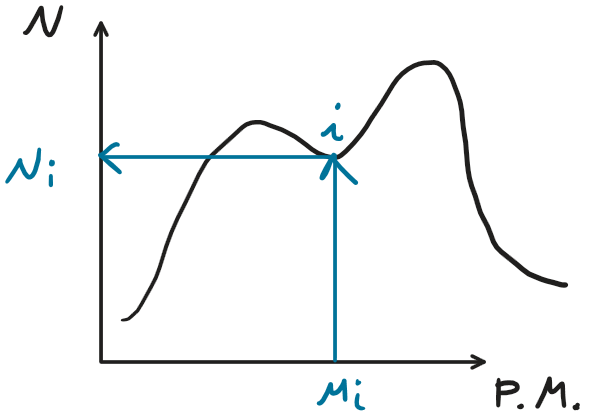
\includegraphics[width = 0.7\textwidth]{gfx/PM}
\caption{Esempio di distribuzione dei pesi molecolari in funzione del numero di moli}
\label{fig:PM}
\end{figure}

$N$ rappresenta il numero di moli con il dato peso molecolare.
In genere si hanno due massimi nella distribuzione del peso molecolare.
Le frazioni a peso molecolare più basso servono a dare al materiale delle proprietà viscose basse.
Quelle a peso molecolare alto per dare le caratteristiche meccaniche.

\section{Peso molecolare medio numerico}
Un primo parametro di caratterizzazione del polimero può essere il peso molecolare medio.
Se 
\begin{equation}
\begin{split}
W &:= \textup{Peso del campione}\\
N &:= \textup{numero totale di moli nel campione}\\
\bar{M}_n &:= \textup{Peso molecolare medio numerico}\\
\phi_i &:= \textup{Frazione molecolare}\\
\bar{M}_n &= \sum_i{\frac{W_i}{N}} = \frac{\sum_i{N_iM_i}}{N} = \sum_i{\frac{N_i}{N}M_i} = \sum_i{\phi_iM_i}
\end{split}
\end{equation}  

\section{Peso molecolare medio ponderale}
\begin{equation}
\begin{split}
\bar{M}_w &:= \textup{peso molecolare medio ponderale}\\
\psi_i &:= \textup{Frazione ponderale}\\
\bar{M}_w &= \sum_i{\frac{W_i}{W}M_i} = \frac{\sum_i{N_iM_i^2}}{W} = \sum_i{\frac{N_iM_i^2}{N_iM_i}} 
\end{split}
\end{equation}

Si può dimostrare che il peso medio ponderale è maggiore del peso medio numerico.
I due pesi medi molecolari sono uguali nel momento in cui entrambi sono uguali a un certo valore $M$.
Si può allora definire un \ac{IPD} detto anche poli-dispersità.
\begin{equation}
IDP = \frac{\bar{M}_w}{\bar{M}_n} \geq 1
\label{eqn:IDP}
\end{equation}
Dalla definizione si osserva che vale $1$ quando il polimero è mono-disperso, poli-disperso altrimenti.

Il peso molecolare medio ponderale è sensibile alle variazioni di frazioni molecolare ad alto peso molecolare.
Il peso molecolare medio numerico sensibile alle variazioni di frazioni molecolari a basso peso molecolare.

\section{Metodi di misura dei pesi molecolari}
Per la misura del peso molecolare di un campione, si scruta la dipendenza della viscosità dal peso molecolare. 
se ne estrae, tramite prove di viscosità, un peso molecolare medio. 
Si può ottenere un'ulteriore misura che permette non solo di valutare i pesi molecolari medi, consentendoci di ottenere direttamente la distribuzione dei pesi molecolari.

Non si possono ricavare con delle misure dirette i pesi molecolari, infatti le misure si realizzano sulla viscosità. 
Si parla di due tipi di viscosità: 
\begin{itemize}
\item viscosità a caldo, dove il materiale viene portato a fusione e ne misura la viscosità
\item viscosità in soluzione, dove si scioglie il materiale in un solvente con viscosità nota e si misura quella del composto misto.
\end{itemize}

\subsection{Melt Flow Index}
Il \ac{MFI} 

%\addtocontents{toc}{\protect\clearpage} % <--- just debug stuff, ignore
%************************************************
\chapter{Comportamento termico}\label{chp:ComportamentoTermico}
%************************************************
Per andare ad analizzare il comportamento termico di un materiale polimerico consideriamo uno completamente amorfo, per il momento. 
Alla figura \ref{fig:Tg}, viene rappresentato il suo comportamento termico.
\graffito{All'aumentare della temperatura, dopo la transizione vetrosa, il materiale abbasserà ulteriormente il suo modulo elastico fino ad arrivare alla condizione di fluido ad alta viscosità}
Dal grafico si rilevano due zone separate dalla temperatura di transizione vetrosa $T_g$.
La prima zona si chiama di \textbf{vetro} ed è la zona in cui il materiale polimerico amorfo presenta il suo massimo modulo elastico.
Nella seconda zona invece si definisce a comportamento \textbf{gomma} in cui il materiale perde la sua caratteristica di modulo elastico, fino ad arrivare alla condizione di fluido ad alta viscosità.

\begin{figure}
\centering
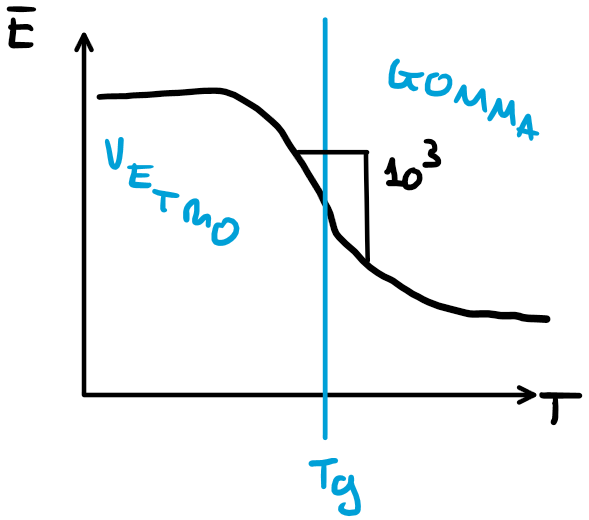
\includegraphics[width = \textwidth]{gfx/Tg}
\caption{Comportamento termico di un materiale amorfo}
\label{fig:Tg}
\end{figure}


Nella realtà, la transizione vetrosa avviene all'interno di un determinato range di temperature. Per convenzione viene fissato la temperatura intermedia a tale range.
A livello microstrutturale non c'è un vero e proprio cambio di struttura nel materiale perché il materiale amorfo era e amorfo rimane.

\begin{figure}
\centering
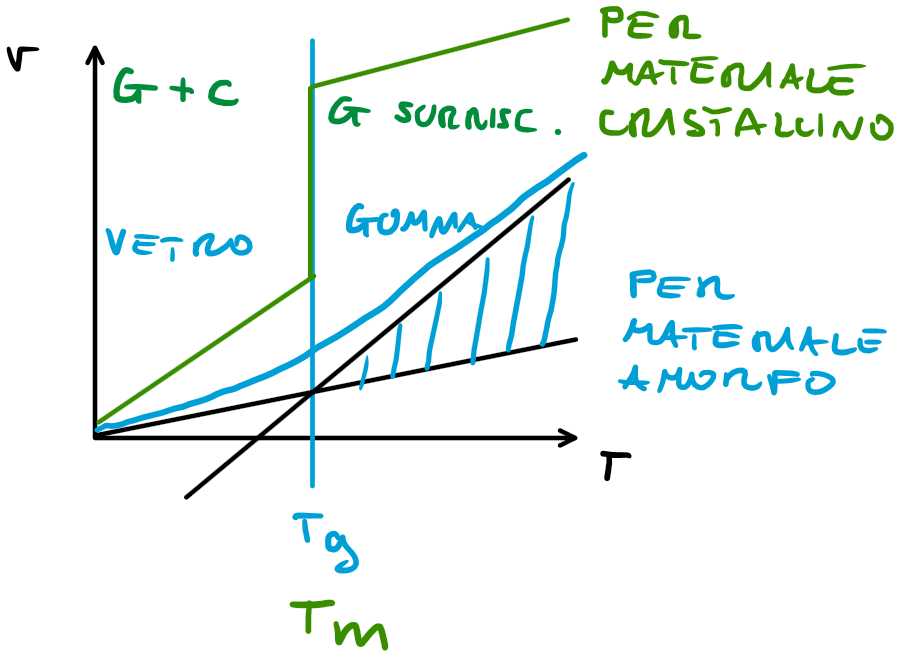
\includegraphics[width = \textwidth]{gfx/VolSpec}
\caption{In termini di volume specifico si vedono in comportamenti per un materiale amorfo e uno semicristallino}
\label{fig:VolSpec}
\end{figure}

Il grafico mostrato in figura \ref{fig:VolSpec}, presenta la variazione del volume specifico in funzione della temperatura sia per un materiale amorfo che per un materiale semi cristallino.
Ciò che accade è che al passaggio attraverso la temperatura di transizione vetrosa $T_g$ aumenta lo spazio libero tra una molecola e l'altra. Determinando, così, una maggiore capacità delle molecole di vibrare attorno ad un punto di equilibrio. Ciò determina anche la repentina diminuzione del modulo elastico. 
Modificando la pressione esterna il comportamento viene traslato verso temperature maggiori, questo perché la pressione limita la vibrazione delle molecole quindi serve più energia per poter ottenere lo stesso comportamento. 

\begin{quote}
\emph{Per un materiale semicristallino?}
\end{quote}


\begin{figure}
\centering
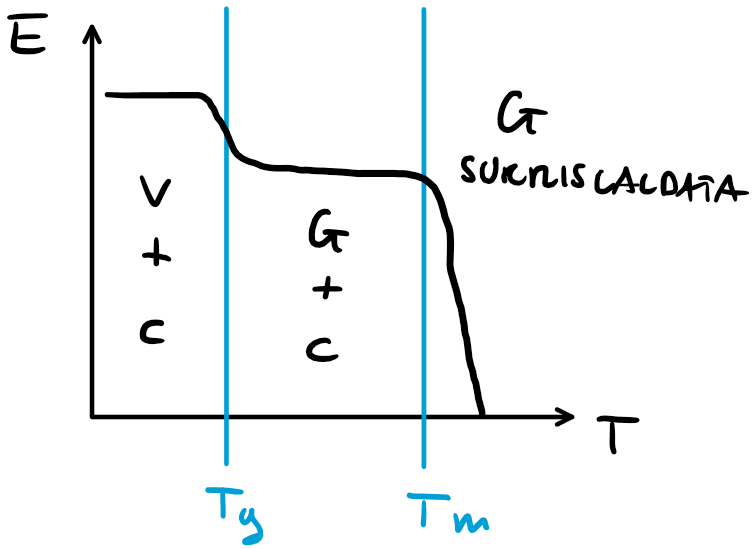
\includegraphics[width = \textwidth]{gfx/TgTm}
\caption{Comportamento termico di un materiale semicristallino}
\label{fig:TgTm}
\end{figure}
Nei materiali semicristallini si ha una vera e propria trasformazione di fase in questo caso si ha una temperatura specifica di trasformazione.

La temperatura di fusione $T_m$ è un unico valore per cui il materiale può essere tranquillamente lavorabile. 
A differenza dei materiali amorfi, la transizione tra materiale cristallino e fluido non risente della pressione in quanto i cristalli sono già compatti.
Dunque, non presentano gli stessi fenomeni evidenziati precedentemente.
 
Per gli amorfi si preferisce oltrepassare il plateau di stato di gomma e avere un materiale molto fluido.
I materiali amorfi vengono utilizzati sempre allo stato vetroso mai gommoso. Sono, tendenzialmente, rigidi e abbastanza resistenti ma fragili. La gomma invece è tendenzialmente duttile e lavorabile.
I materiali cristallini, invece, se utilizzati sotto la temperatura di transizione vetrosa $T_g$ sarebbero materiali eccessivamente fragili. Risulta più conveniente usare all'interno della temperatura di transazione vetrosa e quella di fusione $T_g < T < T_m$. Si ha una gomma rinforzata da cristalli la parte amorfa conferisce tenacità, mentre i cristalli le proprietà meccaniche. 

In generale le plastiche trasparenti sono sempre allo stato vetroso, infatti sono amorfe e di conseguenza fragili. Fa eccezione il \ac{PC} che è a morfo ma non è fragile.
Gli elastomeri sono delle gomme reticolate, per cui conservano le loro proprietà per un buon tratto oltre la temperatura di fusione per via della reticolazione quindi non fondono.

\section{Fattori che influenzano la transizione}
La transizione vetrosa è influenzata da:
\begin{itemize}
\item Mobilità della catena principale,
\item Sostituenti laterali: ingombro e mobilità propria,
\item Legami intermolecolare,
\item Peso molecolare.
\end{itemize}

\paragraph{Mobilità della catena principale}
La transizione vetrosa dipende dalla vibrazione delle molecole attorno alla loro posizione di equilibrio: dunque per catene molto mobili si ha una temperatura di transizione vetrosa più bassa.
Per esempio il \ac{PE} ha una transizione vetrosa a $-100\unit{\celsius}$, decisamente bassa.   
Incrementando la rigidezza della catena polimerica la temperatura di transizione vetrosa aumenta.
Altri materiali:
\begin{itemize}
\item il \ac{PET} ha $T_g = 60\unit{\celsius}$,
\item il \ac{PC} ha $T_g = 120\unit{\celsius}$.
\end{itemize}

\begin{quote}
\emph{Come mai il \ac{PET} lo usiamo a temperatura ambiente anche se risulterebbe vetroso?}
\end{quote}
In questo caso è molto importante il fattore acqua contenuta nell'umidità ambientale.
Tale comportamento, figura \ref{fig:Umidita}, è dovuto ai legami intermolecolari deboli tra le varie catene in cui l'acqua si va ad inserire in mezzo ai legami intermolecolari realizzando una specie di "lubrificazione" tra le molecole. Viene detto \textbf{effetto plastificante}. L'acqua plastifica il polimero, di fatto spezza i legami intermolecolari.
Diminuendo il numero di legami intermolecolari ancora in atto si va a diminuire la temperatura di transizione vetrosa permettendo alle molecole di essere libere a minore energia. 

\begin{figure}
\centering
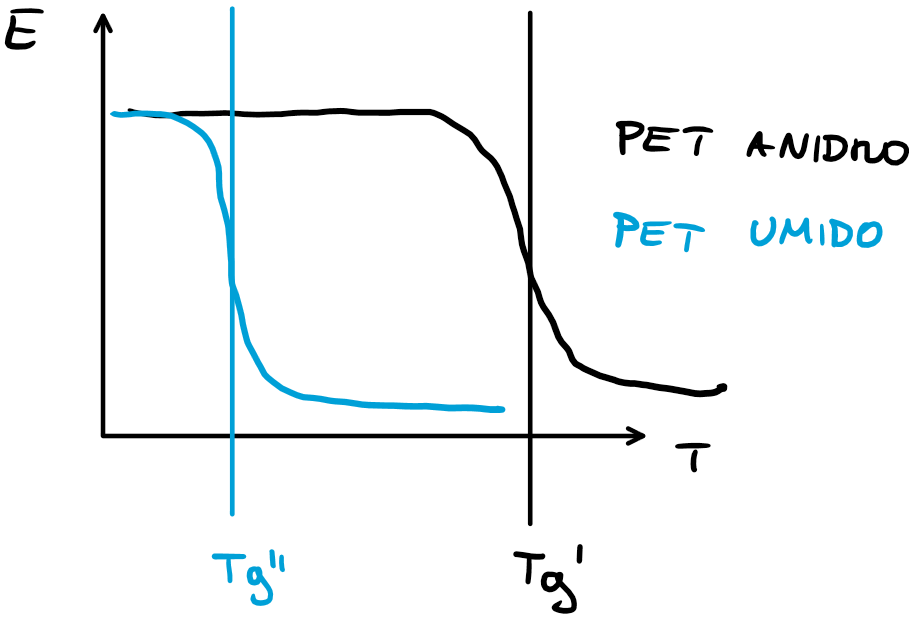
\includegraphics[width = \textwidth]{gfx/Umidita}
\caption{Effetto di abbassamento della transizione per via dell'umidità}
\label{fig:Umidita}
\end{figure}

\paragraph{Sostituenti laterali}
Un sostituente particolarmente ingombrante porta un incremento notevole della $T_g$. Se, per esempio, consideriamo un anello benzenico la temperatura viene aumentata da $-100\unit{\celsius}$ del \ac{PP} a $100\unit{\celsius}$ del \ac{PS}. Mostrati in figura \ref{fig:ConfPPPS}.

\begin{figure}
\centering
\subfloat[][\emph{}\label{fig:PP}]
{%
\begin{minipage}[b]{0.4\textwidth}
\setchemfig{atom sep = 2em}
\schemestart
\chemname{\chemfig{\vphantom{C}-[@{op,.5}]C(-[2]CH_3)(-[6]H)-C(-[2]H)(-[6]H)-[@{cl,.5}]}}{Polipropilene}
\polymerdelim[delimiters ={[]}, indice = n]{op}{cl}
\schemestop
\end{minipage}%
}\quad
\subfloat[][\emph{}\label{fig:PS}]
{%
\begin{minipage}[b]{0.4\textwidth}
\setchemfig{atom sep = 2em}
\schemestart
\chemname{\chemfig{\vphantom{C}-[@{op,.5}]C(-[2]**6(------))(-[6]H)-C(-[2]H)(-[6]H)-[@{cl,.5}]}}{Polistirene}
\polymerdelim[delimiters ={[]}, indice = n]{op}{cl}
\schemestop
\end{minipage}%
}
\caption{Confronto tra i monomeri di polipropilene e polistirene}
\label{fig:ConfPPPS}
\end{figure}

Si può osservare che pur aumentando l'ingombro, se la catena sostituente è molto mobile allora gli effetti si sovrappongono. Il punto è che la mobilità crea molto più volume libero. Dunque l'effetto diventa contrario rispetto a mettere un semplice sostituente. Questo perché bisogna considerare sia il fattore di ingombro che il fattore di mobilità del sostituente in cui la mobilità del sostituente gioca un ruolo più importante.

\paragraph{Legami intermolecolari}
I legami intermolecolari più aumentano in termini di forza e frequenza più la temperatura di transizione vetrosa $T_g$ aumenterà.
Ad esempio il \ac{PVC}, questo genera dei legami intermolecolari più forti. Infatti ha una transizione vetrosa più alta rispetto al polipropilene nonostante siano entrambi materiali vinilici. 

\paragraph{Peso molecolare}
Come era stato anticipato precedentemente, il peso molecolare influisce molto sulla temperatura di transizione vetrosa. Infatti molecole ad alto grado di polimerizzazione avranno sicuramente un peso molecolare più alto ma necessitano di maggiore energia cinetica per potersi muovere.
Siccome necessitano di maggiore energia vuol dire che la temperatura di transizione vetrosa verrà spostata verso valori più alti rispetto a molecole che avendo un grado di polimerizzazione più basso necessiteranno di minore energia per agitarsi.
Risulta essere tutta una questione cinetica.

%************************************************
\chapter{Viscoelasticità}\label{ch:viscoelasticità}
%************************************************
Si tratta della caratterizzazione del comportamento meccanico delle plastiche allo stato solido.

Ipotizzando un materiale solido di cui non si conoscono le caratteristiche meccaniche, la prima prova che si fa è la prova di trazione: si tira e si vede cosa succede.

\begin{quote}
\emph{Si, ma\dots \dots non funziona come per i metalli}
\end{quote}
Infatti si presenta uno sforzo dipendente, si dal carico, anche dalla velocità di deformazione.
In generale, i materiali plastici hanno una forte \textbf{sensibilità alla velocità di deformazione}.
Non è l'unica deviazione dal comportamento dai solidi metallici.

Se un materiale è elastico, allora determinato il modulo elastico, o modulo di Young, si conosce il materiale.
Per le plastiche vale diversamente: se il materiale è completamente amorfo, allora effettivamente l'analisi del modulo elastico è molto significativa per il materiale. Questo però è un caso limite, da non prendere come regola generale.
Dunque, questo tipo di prova non è significativa per i materiali polimerici.

Si preferisce caratterizzarli in altro modo:
\begin{equation}
\sigma = \sigma(\epsilon,\dot{\epsilon})
\end{equation}
ovvero lo sforzo non è determinato solo dalla deformazione ma anche dalla \textbf{velocità di deformazione}.

Allora per caratterizzare il materiale è opportuno misurare proprio le deviazione dal comportamento elastico:
\begin{itemize}
\item Scorrimento viscoso \textbf{Creep},
\item Rilassamento degli sforzi.
\end{itemize}

\paragraph{Rilassamento degli sforzi}
Viene imposta una deformazione costante nel tempo.
Va ricordato che:
\begin{equation}
\epsilon = \frac{L - L_0}{L_0} \quad	\sigma = e(\dot{\epsilon},t)
\end{equation}
Allora il comportamento che si osserva per tale prova è quello delle figure \ref{fig:RilassamentoE} e \ref{fig:RilassamentoS}.

\begin{figure}
\centering
\subfloat[][\emph{Imposizione della deformazione costante}\label{fig:RilassamentoE}]
{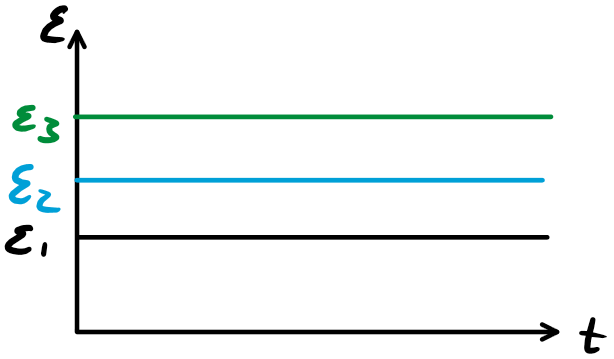
\includegraphics[width = 0.4\textwidth]{gfx/RilassamentoE}}\quad
\subfloat[][\emph{Fenomeno del rilassamento degli sforzi}\label{fig:RilassamentoS}]
{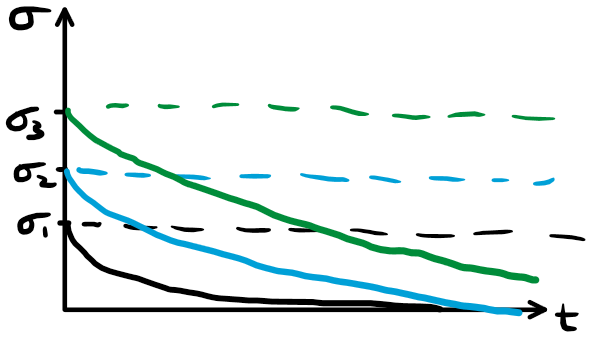
\includegraphics[width = 0.4\textwidth]{gfx/RilassamentoS}}\\
\subfloat[][\emph{Imposizione dello sforzo costante}\label{fig:CreepS}]
{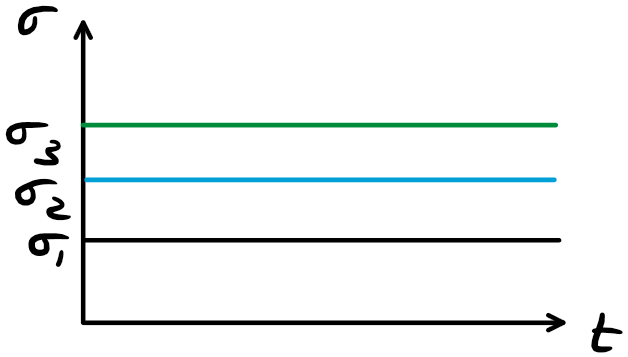
\includegraphics[width = 0.4\textwidth]{gfx/CreepS}}\quad
\subfloat[][\emph{Effetto di \eng{Creep}}\label{fig:CreepE}]
{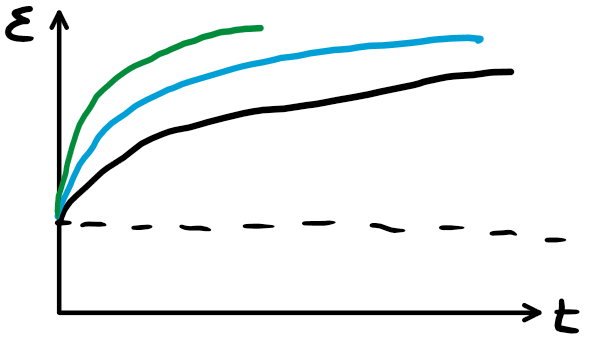
\includegraphics[width = 0.4\textwidth]{gfx/CreepE}}
\end{figure}

\paragraph{Scorrimento viscoso (\eng{Creep})}
Imponendo uno sforzo costante, si osserva l'andamento della deformazione del materiale.

Se la risposta del materiale è lineare, in una delle due variabili, allora la caratterizzazione del materiale può essere più semplice. Sopratutto de il primo degli argomenti di $\bar{\epsilon}$ o $\bar{\sigma}$.

Affinché una funzione sia lineare deve soddisfare entrambe le seguenti:
\begin{align}
f(k*x) &= kf(x) :=\textup{Condizione di funzione omogenea}\\
f(x_1 + x_2) &= f(x_1) + f(x_2) :=\textup{Principio di sovrapposizone degli effetti}
\end{align}

\section{Viscoelasticità lineare}
Ricordando che:
\begin{equation}
\begin{split}
\sigma &= e(\bar{\epsilon}, t) &=\textup{Rilassamento}\label{eqn:Rilassamento}%
\\
\epsilon &= d(\bar{\sigma}, t) &=\textup{\eng{Creep}}
\end{split}
\end{equation}
Ipotizzando che $e$ sia lineare in $\bar{\epsilon}$:
\begin{equation}
e(\bar{\epsilon},t) \rightarrow \bar{\epsilon} * E(t)
\label{eqn:ModuloRilassamento}
\end{equation}
Dove si può definire $E(t)$ come \textbf{Modulo di rilassamento}.
Lo si può ottenere sostituendo nella \eqref{eqn:Rilassamento} la definizione appena trovata \eqref{eqn:ModuloRilassamento}, ottenendo:
\begin{equation}
E(t) = \frac{\sigma(t)}{\bar{\epsilon}}
\end{equation}
Ciò vale solamente in cui il materiale sia linearmente dipendente dalla deformazione.
D'altra parte si può definire un comportamento analogo nel caso:
\begin{equation}
\epsilon(t) = d(\bar{\sigma},t) = \bar{\sigma} * D(t)
\end{equation}
Allora si può definire $D(t)$ come \textbf{Cedevolezza di creep}.
Definito, in maniera analoga al modulo di rilassamento:
\begin{equation}
D(t) = \frac{\epsilon(t)}{\bar{\sigma}}
\end{equation}
Sempre a patto che il materiale presenti una dipendenza lineare allo sforzo applicato.

Valgono anche le seguenti:
\begin{enumerate}
\item Se il materiale è lineare in rilassamento, allora lo è anche in \eng{creep}. Se il materiale è lineare in \eng{creep} allora lo è anche in rilassamento.
\item $E(t)$ e $D(t)$ non sono indipendenti tra loro: misurandone una si ottiene di conseguenza l'altra. Il problema sta nella complessità della relazione tra le due.
\item Misurando tutte e due, si può ottenere il comportamento del materiale anche quando una delle due "costanti" è funzione del tempo. Dunque considerando una storia sforzo/carico arbitraria.
\end{enumerate}
Quindi: il materiale o è lineare o non lo è e non c'è modo di linearizzarlo.

Con le ipotesi di linearità con risposta viscoelastica del materiale,
le equazioni che abbiamo trovato sono:
\begin{align}
\sigma(t) &= E(t)\epsilon_0 + \int_0^t{E(t-s)\dot{\epsilon}(s)\,ds} \label{eqn:RilassamentoComp}\\
\epsilon(t) &= D(t)\sigma_0 + \int_0^t{D(t-s)\dot{\sigma}(s)\,ds}\label{eqn:CreepCompleto}
\end{align}

\subsection{Test per la valutazione se il materiale è lineare}
Le equazioni viste precedentemente evidenziano come il materiale si deformi in maniera lineare, ma il contributo totale è rappresentato da un primo contributo iniziale e poi la storia di deformazione del materiale.

Per valutare la linearità della risposta viscoelastica si va a valutare solamente l'omogeneità della funzione.

Per ipotesi immaginiamo un test di \eng{creep}. Allora per verificare la linearità si fruttano le curve \textbf{isocrone}. 
Si considera un determinato tempo $\bar{t}$ al quale corrisponderà sia un certo carico (costante), sia una certa deformazione che si ottiene tramite le curve di deformazione al \eng{creep}. Si prendono quei valori e li si graficano in una coppia d'assi $\epsilon-\sigma$ come in figura \ref{fig:Isocrone}.

\begin{figure}
\centering
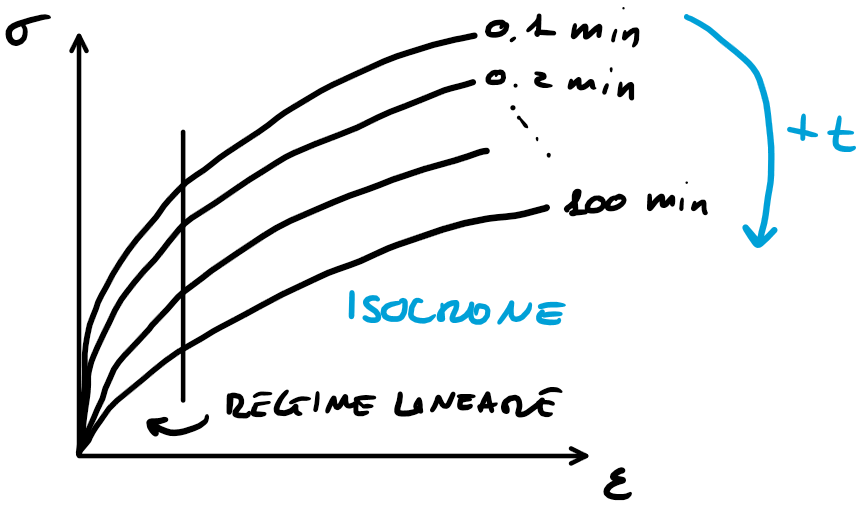
\includegraphics[width = \textwidth]{gfx/Isocrone}
\caption{Schematizzazione delle curve isocrone prese a partire da una prova di \eng{creep}}
\label{fig:Isocrone}
\end{figure}

\paragraph{Osservazioni}
\begin{itemize}
\item Si sarebbe tentati di considerarle delle prove di trazione: ovviamente non lo sono, la modalità di realizzazione è completamente diversa da una mera prova di trazione.
\item Siccome vale:
\begin{equation}
\epsilon(t) = \sigma_iD(t) \rightarrow \epsilon(\bar{t}) = \sigma_iD(t)
\end{equation}
In più \begin{equation}
\frac{\sigma_i}{\epsilon(\bar{t})} = \frac{1}{D(\bar{t})}
\end{equation}
evidenziando come la funzione di effettivamente lineare. Dunque, rappresentabile tramite semirette.
\item Inoltre, come approssimazione ingegneristica, le isocrone ottenute tramite \eng{creep} o come rilassamento siano le stesse. In realtà non è propriamente vero.
\end{itemize}

Come si vede dal grafico \ref{fig:Isocrone}, effettivamente le isocrone non sono propriamente lineari: per deformazioni/sforzi molto alti ci si rende conto del comportamento meno che lineare.
Allora, di solito, si considera che ad una deformazione del $1\% \div 1.5\%$ se le isocrone sono approssimativamente rettilinee, allora il materiale ha comportamento viscoelastico lineare.

Nel caso si vogliano le isocrone a partire da una prova di rilassamento:
\begin{equation}
\begin{split}
\sigma(t) &= \epsilon_iE(t) \rightarrow \sigma(\bar{t}) = \epsilon_iE(\bar{t})\\
\frac{\sigma(\bar{t})}{\epsilon_i} &= E(\bar{t}) = cost.
\end{split}
\end{equation}

\section{Prova di trazione per materiali viscoelastici lineari}
Si impone una deformazione a velocità costante, si misura lo sforzo: $\epsilon(t) = \alpha t$.
In cui $\alpha$ è la \textbf{velocità di deformazione} imposta.
ricordando che:
\begin{equation}
\begin{split}
\sigma(t) &= E(t)\epsilon_0 + \int_0^t{E(t-s)*\dot{\epsilon}(s)\,ds}\\
&=E(t)\epsilon_0 + \int_0^t{E(t-s)*\alpha\,ds} =E(t)\epsilon_0 + \alpha \int_0^t{E(t-s)\,ds}\\
&\Rightarrow \underbrace{\left[t-s = \tau\right]}_{\textup{Cambio variabile}} \Rightarrow\\
&=E(t)\epsilon_0 + \alpha \int_t^0{E(\tau)\,(-d\tau)} = E(t)\epsilon_0 + \alpha \int_0^t{E(\tau)\,d\tau}\\
&= E(t)\epsilon_0 + \alpha \int_0^t{E(s)\,ds}\\
\sigma &= \sigma(t) \rightarrow \sigma = \sigma(\epsilon)
\end{split}
\end{equation}
Dunque, per ottenere lo sforzo in funzione della deformazione:
\begin{equation}
\begin{split}
\epsilon &= \alpha * t \rightarrow t = \epsilon/\alpha\\
\sigma &= \sigma\left(\frac{\epsilon}{\alpha}\right)\\
\sigma &= \alpha \int_0^t{E(s)\,ds}
\end{split}
\end{equation}
Per sapere, indicativamente l'andamento dello sforzo:
\begin{equation}
\begin{split}
\frac{d\sigma}{d\epsilon} = \alpha\frac{d\int}{dE} = \alpha \frac{d\int}{d\frac{\epsilon}{\alpha}}*\frac{d\frac{\epsilon}{\alpha}}{dE}
\end{split}
\end{equation}
Per un materiale viscoelastico lineare presenta un grafico sforzo-deformazione crescente lineare non rettilineo, molto simile alle isocrone senza che lo sia.
la curva di può parametrizzare si $\alpha$ che, in un certo senso, rappresenta il tempo nel caso delle isocrone. In realtà, aumentando la velocità di deformazione il materiale presenta un comportamento più rigido.
\begin{equation}
E_y = \frac{d\sigma}{d\epsilon}\Big|_{\epsilon = 0} = E(0)
\end{equation}
Ci dice che la rigidezza rimane sempre la stessa al variare della velocità do deformazione.
\begin{equation}
\begin{split}
E_y &= \frac{\bar{\sigma}}{\bar{\epsilon}} = \frac{1}{\bar{\epsilon}}\int_0^{\bar{\epsilon}/\alpha}{E(s)\,ds}\\
&= \int_0^{\bar{\epsilon}/\alpha}{E(s)\,ds} - E(\bar{\epsilon}/\alpha) * \bar{\epsilon}/\alpha
\end{split}
\end{equation}

Materiali che sono viscoelastici hanno un comportamento intermedio tra quello di un fluido e quello di un solido. Il comportamento è tipico delle plastiche allo stato solido.

\section{Fluidi e solidi viscoelastici}
Un fluido viscoelastico ha un modulo di rilassamento pari a 0. Per cui dato uno sforzo, il fluido andrà a deformazione permanente.
Un solido viscoelastico, al contrario, ha modulo di rilassamento finale strettamente positivo.

$D_0$ è legato all'elasticità istantanea che si verifica per tempi relativamente brevi. Se il materiale è un solido viscoelastico, la risposta sarà vincolata ad un asintoto orizzontale.
Se invece è un fluido visco elastico, la sua risposta non è limitata, per cui la cedevolezza di \eng{creep} non è limitata superiormente.

%************************************************
\chapter{Legame tra modulo di rilassamento e cedevolezza di \eng{creep}}%
\label{chp:LegameCedevolezzaCreep}
%************************************************
\section{Prova di \eng{creep}}
Da un punto di vista dimensionale sono l'uno il reciproco dell'altro.
\begin{equation}
\sigma(t) = E(t)\epsilon_0 + \int_0^t{E(t-s)*\dot{\epsilon}(s)\,ds}
\end{equation}
Questa vale anche nel caso della prova di \eng{creep}: lo sforzo sarà costante:
\begin{equation}
\sigma(t) = \bar{\sigma} \qquad \epsilon(t) = \bar{\sigma} D(t)
\end{equation}
Dunque:
\begin{equation}
\begin{split}
\bar{\sigma} &= E(t) * \bar{\sigma} * D(0) + \int_0^t{E(t-s)\bar{\sigma}\dot{D}(s)\,ds}\\
1 &= E(t) * D(0) + \int_0^t{E(t-s)\dot{s}\,ds}
\end{split}
\end{equation}
Eventuali approssimazioni:
\begin{equation}
t \rightarrow 0
\end{equation}
Allora:
\begin{equation}
1 = E(0) * D(0) \rightarrow E(0) = \frac{1}{D(0)}
\end{equation}
Il comportamento di questo materiale è elastico: prevale la componente conservativa che non quella dissipativa. per tempi molto piccoli.
Ipotizzando un tempo generico, allora: $E(t-s) > E(t)$ perché la funzione modulo di rilassamento è una funzione decrescente.
\begin{equation}
\begin{split}
1 &= E(t)D(0) + \int_0^t{E(t-s)\dot{D}(s)\,ds}\\
1 &> E(t)D(0) + \int_0^t{E(t)\dot{D}(s)\,ds}\\
&= E(t)D(0) + E(t)[D(t)-D(0)] = E(t) * D(t) \rightarrow D(t) \leq \frac{1}{E(t)}
\end{split}
\end{equation}
Tale conferma anche la condizione precedente, infatti per tempi prossimi a 0 si ha una maggior componente elastica che no dissipativa.

Ora ipotizzando che: $\epsilon(t) = \alpha t$ allora:
\begin{equation}
\begin{split}
\alpha t &= D(t) * 0 + \int_0^t{D(t-s)*\alpha*E(s)\,ds}\\
t &= \int_0^t{D(t-s)E(s)\,ds}
\end{split}
\end{equation}
Siccome $D(t-s) \leq D(t)$ perché è una funzione crescente come si vede in figura \ref{fig:Creep}
\begin{figure}
\centering
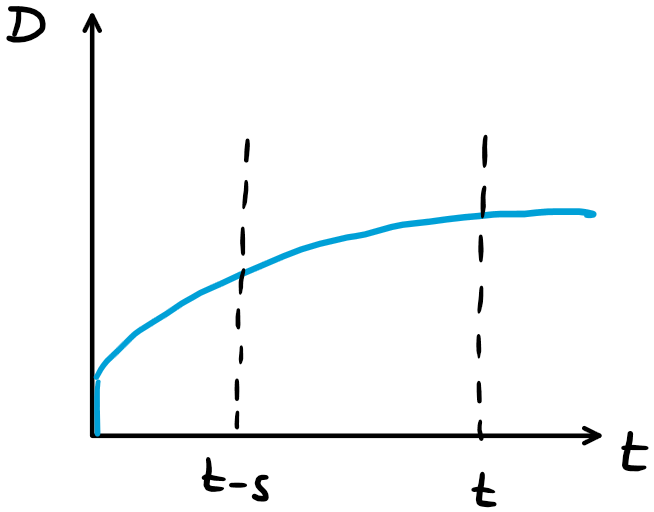
\includegraphics[width = 0.5\textwidth]{gfx/Creep}
\caption{Approssimazione dell'andamento del \eng{creep} per un materiale viscoelastico}
\label{fig:Creep}
\end{figure}
Allora resta valido:
\begin{equation}
t = \int_0^t{D(t-s)E(s)\,ds} \leq \int_0^t{D(t)E(s)\,ds} = D(t)\int_0^t{E(s)\,ds}
\end{equation}
Da cui
\begin{equation}
D(t) \geq \frac{t}{\int_0^t{E(s)\,ds}}
\end{equation}
Lo si può anche scrivere come:
\begin{equation}
D(t) \geq \frac{1}{\underbrace{\frac{1}{t}\int_0^t{E(s)\,ds}}_{\textup{è un valore medio}}}
\end{equation}
Dunque:
\begin{equation}
\begin{split}
\frac{1}{\frac{1}{t}\int_0^t{E(s)\,ds}} \leq D(t) \leq \frac{1}{E(t)}\\
\frac{1}{\bar{E}} \leq D(t) \leq \frac{1}{E(t)}
\end{split}
\end{equation}
Per cui possiamo dire che 
\begin{equation}
D(t) \approx \frac{1}{E(t)}
\end{equation}

Considerando ora $t \rightarrow \infty$: se il materiale è un solido viscoelastico, allora il materiale presenta un asintoto diverso da zero:
\begin{equation}
\exists D_{\infty} < \infty \quad \exists E_{\infty} \neq 0
\end{equation}
Ricordando:
\begin{equation}
\frac{1}{\frac{1}{t}\int_0^t{E(s)\,ds}} \leq D(t) \leq \frac{1}{E(t)}
\end{equation}
Portandolo verso tempi molto lunghi possiamo scrivere che:
\begin{equation}
\frac{\int_0^t{E(s)\,ds}}{t} \, \overrightarrow{t \rightarrow \infty} \, \frac{E(t)}{1}\rightarrow E_{\infty}
\end{equation}
Allora:
\begin{equation}
1 \leq D_{\infty} \leq \frac{1}{E_{\infty}}
\end{equation}

\paragraph{Riassumendo}
Per tempi piccoli il materiale si comporta come se fosse completamente elastico, in quanto cedevolezza e modulo di rilassamento sono l'uno il reciproco dell'altro.
Per tempi intermedi di sforzo ha comportamento viscoelastico.
Per tempi molto più lunghi il materiale si comporterà nuovamente a carattere elastico
\begin{description}
\item[Tempi brevi] \textbf{Comportamento elastico}
\item[Tempi intermedi] \textbf{Comportamento viscoelastico} ovvero ha componente sia elastica che dissipativa.
\item[Tempi lunghi] \textbf{Comportamento elastico}
\end{description}

\section{Prova di rilassamento}
Idealmente saremmo in grado di deformare istantaneamente il materiale, evidentemente ciò non è possibile perché il materiale tende a comportarsi in maniera diversa.
Dunque bisogna utilizzare una rampa di deformazione, da cui si stima il modulo di rilassamento, capendo quanto si sta sbagliando e come.
Allora:
\begin{equation}
\epsilon(t)=%
\begin{cases}
\frac{\bar{\epsilon}}{t}t &0<t<\bar{t}\\
\bar{\epsilon} &t>\bar{t}
\end{cases}
\label{eqn:ProvaRilassamento}
\end{equation}

\begin{figure}
\centering
\subfloat[][\emph{Profilo della deformazione}\label{fig:ProfiloDeformazione}]%
{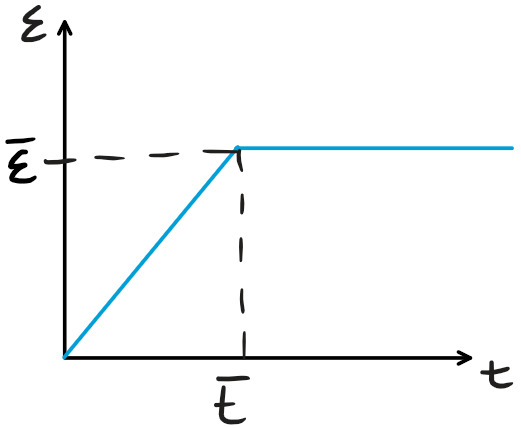
\includegraphics[width = 0.4\textwidth]{gfx/ProfiloDeformazione}}\quad
\subfloat[][\emph{Profilo dello sforzo conseguente}\label{fig:ProfiloSforzo}]%
{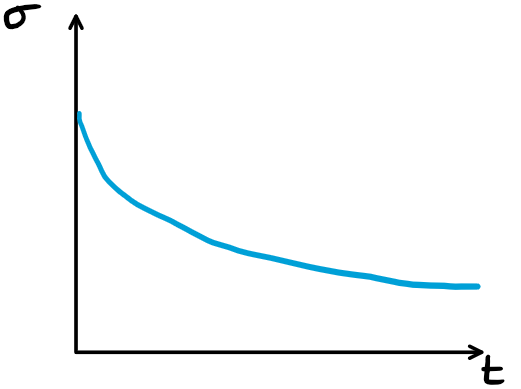
\includegraphics[width = 0.4\textwidth]{gfx/ProfiloSforzo}}	
\caption{Prova di rilassamento}
\label{fig:ProvaRilassamento}
\end{figure}
Conviene separare i due momenti come evidenziato dall'equazione \eqref{eqn:ProvaRilassamento}.

\begin{description}
\item[$0<t<\bar{t}$]
\begin{equation}
\begin{split}
\epsilon(t)&=\frac{\bar{\epsilon}}{\bar{t}}t \quad \dot{\epsilon}=\frac{\bar{\epsilon}}{\bar{t}}\\
\sigma(t)&=\frac{\bar{\epsilon}}{\bar{t}}\int_0^t{E(s)\,ds}\\
\bar{\sigma}(t)&=\sigma(\bar{t})=\frac{\bar{\epsilon}}{\bar{t}}\int_0^{\bar{t}}{E(s)\,ds}
\end{split}
\end{equation}
Il risultato di questo integrale è quello della figura \ref{fig:tMinBar}
\item[$t>\bar{t}$]
\begin{equation}
\begin{split}
\epsilon(t)&=\bar{\epsilon} \quad \dot{\epsilon}(t)=0\\
\sigma(t)&=E(t)\epsilon_0 + \int_0^t{E(t-s)\dot{\epsilon}(s)\,ds}\\
&=\int_0^{\bar{t}}{E(t-s)\dot{\epsilon}(s)\,ds} + \int_{\bar{t}}^t{E(t-s)\dot{\epsilon}(s)\,ds}\\
\sigma(t)&=\int_0^{\bar{t}}{E(t-s)\,ds} \quad\overrightarrow{\tau = t-s}\quad \frac{\bar{\epsilon}}{\bar{t}}\int_t^{t-\bar{t}}{E(\tau)\,(-d\tau)}\\
&= \frac{\bar{\epsilon}}{\bar{t}}\int_{t-\bar{t}}^t{E(s)\,ds}
\end{split}
\end{equation}
Il risultato di questo risultato è \ref{fig:tMagBar}.
\item[$t=\bar{t}$]
\begin{equation}
\begin{split}
\sigma^+(t) &= \frac{\bar{\epsilon}}{\bar{t}}\int_0^{\bar{t}}{E(s)\,ds}\\
\frac{d\sigma}{dt}&=\frac{\bar{\epsilon}}{\bar{t}}(E(t)-E(t-\bar{t}))<0\\
\frac{d^2\sigma}{dt^2}&=\frac{\bar{\epsilon}}{\bar{t}}(\dot{E}(t)-\dot{E}(t-\bar{t})\geq 0\\
\bar{E}(t)&= \frac{\sigma(t)}{\bar{\epsilon}} \quad \leftrightarrow \quad E(t)\\
\bar{E}&=\frac{\sigma(t)}{\bar{\epsilon}} = \frac{1}{\bar{\epsilon}}\frac{\bar{\epsilon}}{\bar{t}}\int_{t-\bar{t}}^t{E(s)\,ds}\\
&=\frac{1}{\bar{t}}\int_{t-\bar{t}}^t{E(s)\,ds}\lesseqgtr E(t)\bar{t}\\
F(t)&\rightarrow \bar{E}(t)-E(t) = \frac{1}{\bar{t}}\int_{t-\bar{t}}^t{E(s)\,ds} - E(t)\\
\frac{dF}{dt} &= \frac{1}{\bar{t}}\left(E(t)-E(t-\bar{t})\right)-\dot{E}(t)<0
\end{split}
\end{equation}
In questo p[unto si vuole dimostrare la continuità della funzione sforzo e si valuta il successivo andamento della continuità come nella figura \ref{fig:tMagBar}.
Inoltre, viene dimostrata dalla figura \ref{fig:ValutazioneEccesso} che l'approssimazione che stiamo seguendo è per eccesso.
In più si osserva che l'errore si assottiglia man mano che si va avanti col tempo, come si vede in figura \ref{fig:ValutazioneErrore}.
Mentre, la figura. \ref{fig:DimostrazioneIntegrali} si fa notare dal punto di vista geometrico il significato dell'ultima riga.
\end{description}

\begin{figure}
\centering
\subfloat[][\emph{Andamento dello sforzo per $0<t<\bar{t}$}\label{fig:tMinBar}]%
{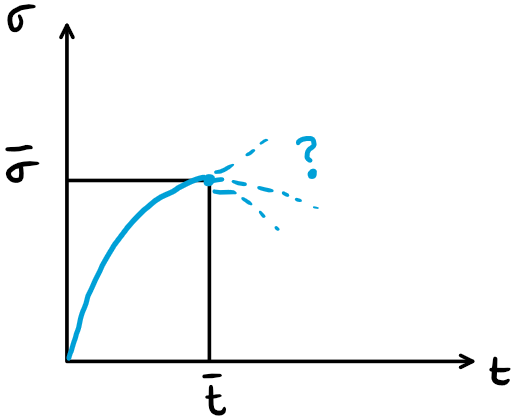
\includegraphics[width = 0.4\textwidth]{gfx/tMinBar}}\quad
\subfloat[][\emph{Andamento dello sforzo per $t>\bar{t}$}\label{fig:tMagBar}]%
{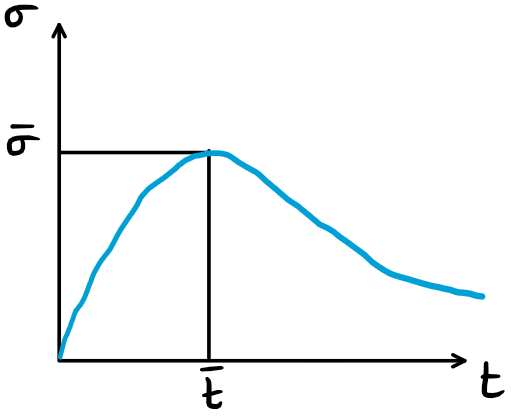
\includegraphics[width = 0.4\textwidth]{gfx/tMagBar}}\\
\subfloat[][\emph{Valutazione dell'errore commesso per via della natura della prova}\label{fig:ValutazioneErrore}]%
{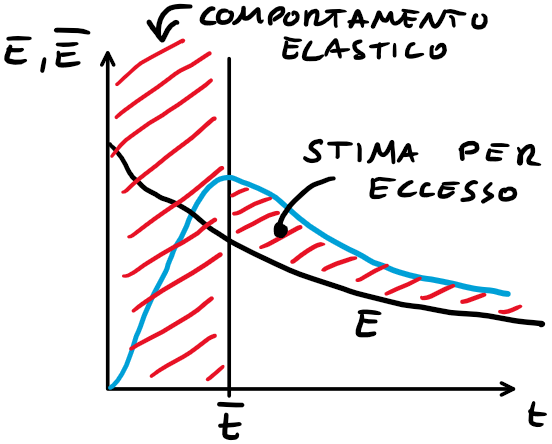
\includegraphics[width = 0.4\textwidth]{gfx/ValutazioneErrore}}\quad
\subfloat[][\emph{Dimostrazione dell'errore per eccesso}\label{fig:ValutazioneEccesso}]%
{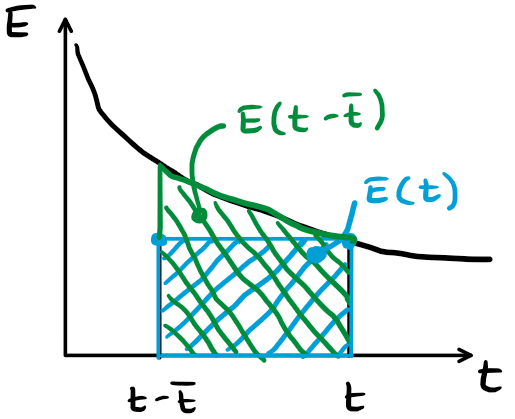
\includegraphics[width = 0.4\textwidth]{gfx/ValutazioneEccesso}}\\
\subfloat[][\emph{Dimostrazione geometrica degli integrali}\label{fig:DimostrazioneIntegrali}]%
{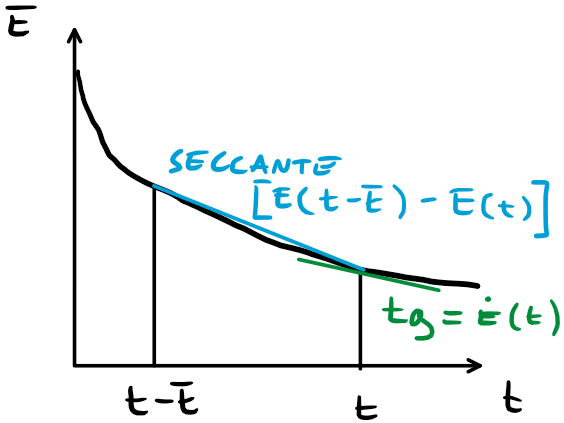
\includegraphics[width = 0.4\textwidth]{gfx/DimostrazioneIntegrale}}	
\caption{Prova di rilassamento reale}
\label{fig:ProvaRilassamento}		
\end{figure}

La prova di rilassamento con rampa, commette un errore per eccesso per via della natura della prova. Per tempi sufficientemente lunghi si abbassa l'effetto dell'errore.
Quando si considerano tempi ben più grandi di quello della rampa (di solito dura qualche secondo) la differenza tra \textbf{stima del modulo di rilassamento} e \textbf{modulo di rilassamento} non è così evidente.
Per avere dei dati per una durata maggiore, si usa alzare la temperatura del materiale. In questo modo si simula il comportamento di ore per una prova di qualche minuto.
Nel caso si vogliano informazioni su anni di esercizio, questi vengono interpolati dalle varie prove.

%************************************************
\chapter{Modelli dei fluidi viscoelastici}\label{chp:ModelliFluidi}
%************************************************
I modelli descritti in letteratura sono una combinazione di elementi \textbf{elastici} e \textbf{dissipativi}.
La viscoelasticità è un comportamento misto, parzialmente elastico e parzialmente dissipativo.
Dunque:
\begin{quote}
\emph{Quando vale il modulo di rilassamento $E(t)$ e il modulo di cedevolezza al \eng{creep} $D(t)$?}
\end{quote}

Allora conviene considerare i due elementi fondamentali:

\begin{figure}
\centering
\subfloat[][\emph{Parametrizzazione come molla per effetti elastici}\label{fig:Molla}]%
{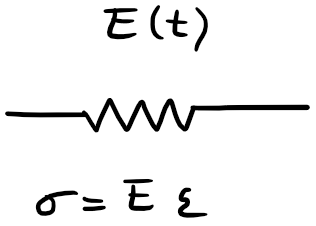
\includegraphics[width = 0.4\textwidth]{gfx/Molla}}\quad
\subfloat[][\emph{Parametrizzazione come smorzatore per gli effetti dissipativi}\label{fig:Dissipatore}]%
{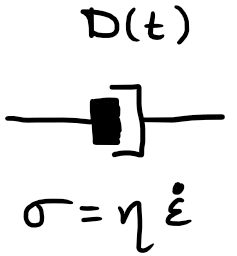
\includegraphics[width = 0.4\textwidth]{gfx/Dissipatore}}	
\caption{Elementi di modellazione dei fluidi viscoelastici}
\label{fig:FluidiViscoelastici}	
\end{figure}

Tra l'altro si vuole ricordare che:
\begin{equation}
\begin{split}
\sigma = \eta \dot{\epsilon} &\textup{Sforzo normale}\\
\tau = \eta \dot{\gamma} &\textup{Sforzo di taglio}
\end{split}
\end{equation}

\section{Fluido di Maxwell}
Rappresentato in figura \ref{fig:FluidoMaxwell}.
\begin{figure}
\centering
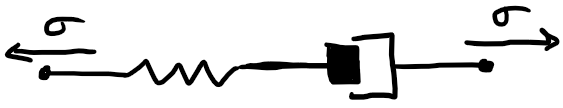
\includegraphics[width = \textwidth]{gfx/FluidoMaxwell}
\caption{Schematizzazione del fluido di Maxwell}
\label{fig:FluidoMaxwell}
\end{figure}

\begin{equation}
\sigma = \sigma_1 = \sigma_2
\end{equation}
Lo sforzo su, rispettivamente, molla e smorzatore.
Mentre la deformazione è:
\begin{equation}
\epsilon = \epsilon_1 + \epsilon_2
\end{equation}
Siccome:
\begin{equation}
\sigma_1 = E*\epsilon_1 \qquad \sigma_2=\eta \dot{\epsilon}_2
\end{equation}
Da cui:
\begin{equation}
\dot{\epsilon} = \dot{\epsilon}_1 + \dot{\epsilon}_2 = \frac{\dot{\sigma}_1}{E} + \frac{\sigma_2}{\eta} = \frac{\dot{\sigma}}{E} + \frac{\sigma}{\eta}
\end{equation}

Dunque:
\begin{equation}
\epsilon = \bar{\epsilon} \rightarrow%
\begin{cases}
\frac{\dot{\sigma}}{E}+\frac{\sigma}{\eta} = 0\\
\sigma_0 = E \cdot \bar{\epsilon}
\end{cases}
\end{equation}
con le seguenti condizioni iniziali:
\begin{equation}
\begin{split}
t&=0\\
\sigma &= E \cdot \bar{\epsilon}
\end{split}
\end{equation}
Risolvendo il sistema di equazioni differenziali:
\begin{equation}
\begin{split}
\frac{d\sigma}{dt} &+ \frac{E}{\eta} \sigma = 0\\
\frac{d\sigma}{dt} &= -\frac{E}{\eta} \sigma \Rightarrow \int{\frac{d\sigma}{\sigma}} = \int{-\frac{E}{t}t}\\
\ln(\sigma)&= -\frac{E}{\eta}t + K \Rightarrow \sigma = e^{-\frac{E}{\eta}t+K}\\
\sigma &= C e^{-\frac{E}{\eta}t}\\
\sigma(0) &= C = E\bar{\epsilon}\\
\sigma(t) &= E\bar{\epsilon}e^{-\frac{E}{\eta}t}\\
E&= \frac{\sigma(t)}{\bar{\epsilon}}=Ee^{-\frac{E}{\eta}t}
\end{split}
\end{equation}
Dove:
\begin{equation}
\tau_r = \frac{\eta}{E} := \textup{ Tempo di rilassamento}
\end{equation}
Da cui infine:
\begin{equation}
E=E_0 e^{-\frac{t}{\tau_r}}
\end{equation}
Il quale comportamento è rappresentato dalla figura \ref{fig:RilassamentoMaxwell}
\begin{figure}
\centering
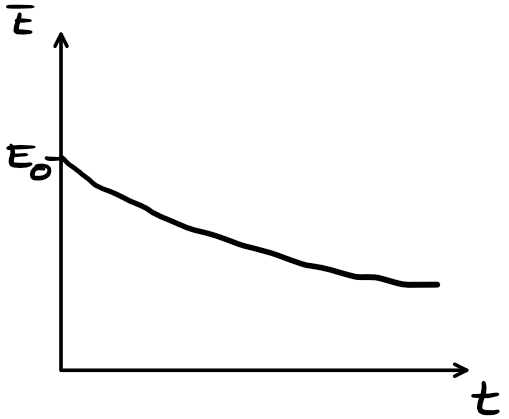
\includegraphics[width = 0.5\textwidth]{gfx/RilassamentoMaxwell}
\caption{Andamento del fluido di Maxwell in termini di rilassamento}
\label{fig:RilassamentoMaxwell}
\end{figure}

Grazie a questi modelli si riesce a capire come funziona anche senza fare calcoli.
Se si tira la molla in serie con un dissipatore, si allunga la molla, ma mano a mano che passa il tempo, tutto il carico preso dalla molla verrà rilassato dal dissipatore viscoso che inizierà a muoversi finché la tensione rimanente verrà rilassata completamente.
La storia di carico è moto prevedibile per via della semplicità del materiale.
\begin{equation}
E(t) = E_0 e^{-\frac{t}{\tau_r}}
\end{equation}
Valutiamo il comportamento al \eng{creep}.
\subsection{Prova di \eng{creep}}
Ricordiamo:
\begin{equation}
\dot{\epsilon} = \frac{\dot{\sigma}}{E} + \frac{\sigma}{\eta}, \quad \sigma = \bar{\sigma} \quad \forall t > 0
\end{equation}
La condizione iniziale:
\begin{equation}
\dot{\epsilon} = \frac{0}{E} + \frac{\bar{\sigma}}{\eta} = \frac{\bar{\sigma}}{\eta} \Rightarrow \epsilon(0)=\frac{\bar{\epsilon}}{E}
\end{equation}
Risolvendo l'equazione differenziale:
\begin{equation}
\epsilon(t) = \frac{\bar{\sigma}}{\eta}t + C \rightarrow \epsilon(0) = \frac{\bar{\sigma}}{E} = C \rightarrow \epsilon(t) = \frac{\bar{\sigma}}{\eta}t + \frac{\bar{\sigma}}{E}
\end{equation}
Siccome
\begin{equation}
D(t) = \frac{\epsilon(t)}{\bar{\sigma}} = \frac{t}{\eta} + \frac{1}{E}
\end{equation}
Si dimostra un fluido viscoelastico perché la deformazione non è limitata e la cedevolezza iniziale ha un valore iniziale diverso da zero..
Infatti, il materiale, eccitato istantaneamente, ha comportamento elastico.

Il fluido di Maxwell è un modello che approssima molto bene il comportamento dei fluidi. Quando il materiale ha comportamento governato dalla viscoelasticità.
Nella realtà si utilizza questo modello, opportunamente riadattato.
Non va assolutamente usato per materiali polimerici allo stato solido.

\begin{figure}
\centering
\subfloat[][\emph{Caratterizzazione del rilassamento del fluido in funzione del rilassamento}\label{fig:TempoRilassamento}]%
{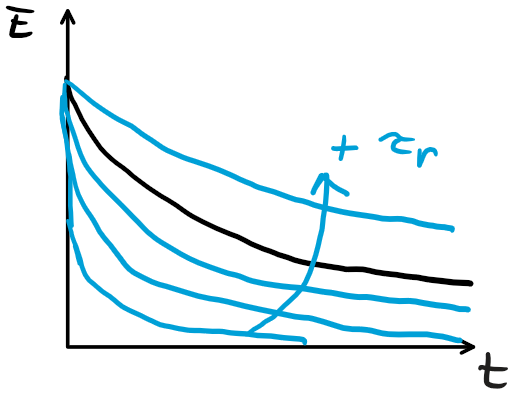
\includegraphics[width = 0.4\textwidth]{gfx/TempoRilassamento}}\quad	
\subfloat[][\emph{Comportamento al \eng{creep}}\label{fig:ComportamentoCreep}]%
{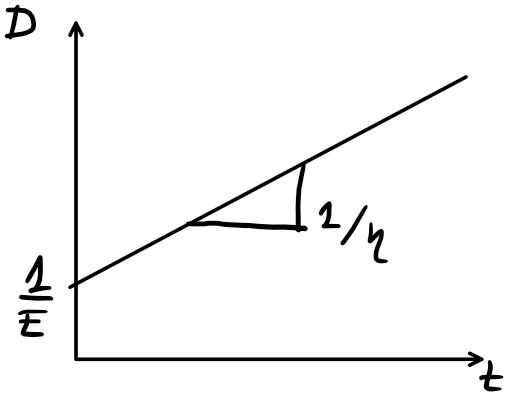
\includegraphics[width = 0.4\textwidth]{gfx/ComportamentoCreep}}	
\caption{Comportamenti del fluido di Maxwell}
\label{fig:ComportamentoMaxwell}
\end{figure}

\section{Modello di Kelvin-Voigt}

\begin{figure}
\centering
\subfloat[][\emph{Modello di \eng{Kelvin-Voigt}}\label{fig:KelvinVoigt}]%
{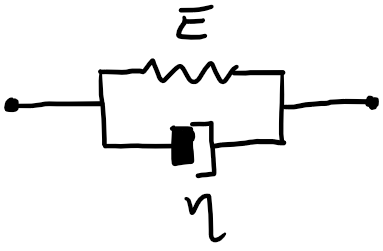
\includegraphics[width = 0.4\textwidth]{gfx/KelvinVoigt}}\quad
\subfloat[][\emph{Descrizione del modello}\label{def:KelvinVoigt}]%
{%
\begin{minipage}[b]{0.4\textwidth}
\begin{description}
\item[$E$] Modulo di Young della molla.
\item[$\eta$] Viscosità elemento dissipativo.
\end{description}
\end{minipage}%
}		
\caption{Modello di \eng{Kelvin-Voigt}}
\label{des:KelvinVoigt}
\end{figure}

La deformazione dell'elemento deve essere uguale per i due rami di molla e smorzatore.
Lo sforzo totale sarà pari alla somma degli sforzi dei due.
\begin{equation}
\begin{split}
\sigma = \sigma_1 + \sigma_2\\
\sigma_1 = E \epsilon_1, \quad \sigma_2 = \eta \dot{\epsilon}_2
\end{split}
\end{equation}
Ne deriva:
\begin{equation}
\sigma = E \epsilon + \eta \dot{\epsilon}
\end{equation}
\subsection{Prova di \eng{creep}}
\begin{equation}
\sigma = \bar{\sigma} \quad \forall t > 0
\end{equation}
Da cui:
\begin{equation}
\eta \dot{\epsilon} + E \epsilon = \bar{\sigma} \Rightarrow \dot{\epsilon} + \frac{E}{\eta}\epsilon = \frac{\bar{\sigma}}{\eta}
\end{equation}
Da cui la condizione iniziale per $\epsilon(0) = 0$
Il comportamento in questo caso se si applica un carico istantaneo si dovrebbe avere una deformazione della sola molla.
Siccome i due elementi sono in parallelo, prevale che: essendo lo smorzatore infinitamente rigido, allora la deformazione sarà nulla.

\begin{equation}
\begin{cases}
 \dot{\epsilon} + \frac{E}{\eta}\epsilon = \frac{\bar{\sigma}}{\eta} \rightarrow \epsilon(t) = \epsilon_h(t) + \epsilon_p(t)\\
\epsilon_p=\frac{\bar{\sigma}}{E}
\end{cases}
\end{equation}
Come si vede, l'equazione differenziale è non omogenea, dunque va calcolata:
\begin{equation}
\begin{split}
\dot{\epsilon}_h &+ \frac{E}{\eta}\epsilon_h = 0 \rightarrow \epsilon_h = K e^{-\frac{E}{\eta}t}\\
\epsilon(t) &= K e^{-\frac{E}{\eta}t}+\frac{\bar{\sigma}}{E} \rightarrow \epsilon(0) = K + \frac{\bar{\sigma}}{E} = 0 \rightarrow K = -\frac{\bar{\sigma}}{E}\\
\epsilon(t) &= -\frac{\bar{\sigma}}{E}e^{\frac{E}{\eta}t}+\frac{\bar{\sigma}}{E} = \frac{\bar{\sigma}}{E}\left(1-e^{-\frac{E}{\eta}t}\right)\\
D(t) &= \frac{\epsilon(t)}{\bar{\sigma}} = \frac{1}{E}\left(1-e^{-\frac{E}{\eta}t}\right) = D_{\infty}\left(1-e^{-\frac{t}{\tau_c}}\right)
\end{split}
\end{equation}
Dove, $\tau_c = \frac{\eta}{E}$ è il tempo di ritardo.

È un solido viscoelastico perché la cedevolezza è superiormente limitata.
Il materiale è istantaneamente rigido: risponde alla sollecitazione istantanea in maniera rigida.
Si osserva che però il modello è patologico perché:
per il comportamento a rilassamento: $\epsilon(t) = \bar{\epsilon}$ allora,
\begin{equation}
\sigma = E\epsilon + \eta \dot{\epsilon} = E \bar{\epsilon}
\end{equation}
Da cui:
\begin{equation}
E(t) = \frac{\sigma(t)}{\bar{\epsilon}} = E
\end{equation}
Non è accettabile che il modello di rilassamento resti costante.
%\include{multiToC} % <--- just debug stuff, ignore for your documents
\ctparttext{Parte delle lezioni svolte dalla professoressa \myOtherProf}
\cleardoublepage \part{Fluidi non newtoniani}
%%%%%%%%%%%%%%%%%%%%%%%%%%%%%%%%%%%%%%%%%%%%%%%%%%%%%%%%%%%%%%%%%%%%%%%%%%%%%%%
\chapter{Fluidi non newtoniani}\label{chp:NonNewton}
%%%%%%%%%%%%%%%%%%%%%%%%%%%%%%%%%%%%%%%%%%%%%%%%%%%%%%%%%%%%%%%%%%%%%%%%%%%%%%%
I materiali polimerici non possiedono comportamento newtoniano.
Possiamo definire come "newtoniano" un fluido per il quale:
\begin{description}
\item[Fluido newtoniano] la viscosità dipende unicamente da temperatura e pressione: $\eta = \eta(T,p)$
\end{description}

Una prima relazione che lega la viscosità a temperatura e pressione può essere quella di \textit{Arrhenius}:
\begin{equation}
\eta = \eta_t e^{\frac{\Delta E}{R}\left(\frac{1}{T}-\frac{1}{T_0}\right)} %
e^{\beta \left(p - p_0\right)}
\label{eqn:Arrhenius}
\end{equation}
Resta evidente come:
\begin{itemize}
\item Se $p \uparrow\uparrow$ allora $\eta \uparrow\uparrow$.
\item Se $T \uparrow\uparrow$ allora $\eta \downarrow\downarrow$. 
\end{itemize}

Nello specifico, i fluidi non newtoniani presentano delle così dette \textbf{deviazioni} dal comportamento del fluido newtoniano.
Ora verranno elencate e poi approfondite nello stesso ordine.

\begin{enumerate}
\item La viscosità dipende dalle condizioni di flusso, in particolare dalla velocità di deformazione.
\item Possono esserci effetti di sforzo normale.
\item Possono esserci effetti di viscoelasticità.
\item Possono esserci effetti di plasticità: ovvero fenomeni di snervamento.
\item Gli effetti sono conseguenze del tempo: \textbf{tissotropia}.
\end{enumerate}

\section{Condizioni di flusso}
Come accennato in precedenza, una deviazione dal comportamento di fluido newtoniano può essere quella della dipendenza dalle condizioni di flusso alle quali il fluido viene sottoposto.
In particolare i fluidi non newtoniani dipendono fortemente dalla velocità di deformazione $\dot{\gamma}$.
Perciò, vale:
\begin{equation}
\eta = \eta(\dot{\gamma})
\label{eqn:viscNonNewt}
\end{equation}
Funzione che lega la viscosità con la velocità di deformazione.
Siccome lo \textbf{sforzo di taglio} vale, sia per fluidi newtoniani che non:
\begin{equation}
\tau = \eta \dot{\gamma}
\label{eqn:sforzoTaglio}
\end{equation}
Da cui, sostituendo la \eqref{eqn:viscNonNewt} alla \eqref{eqn:sforzoTaglio} ne risulta:
\begin{equation}
\tau = \eta(\dot{\gamma}) \dot{\gamma}
\label{eqn:taglioNonNewt}
\end{equation}

\begin{figure}
\centering
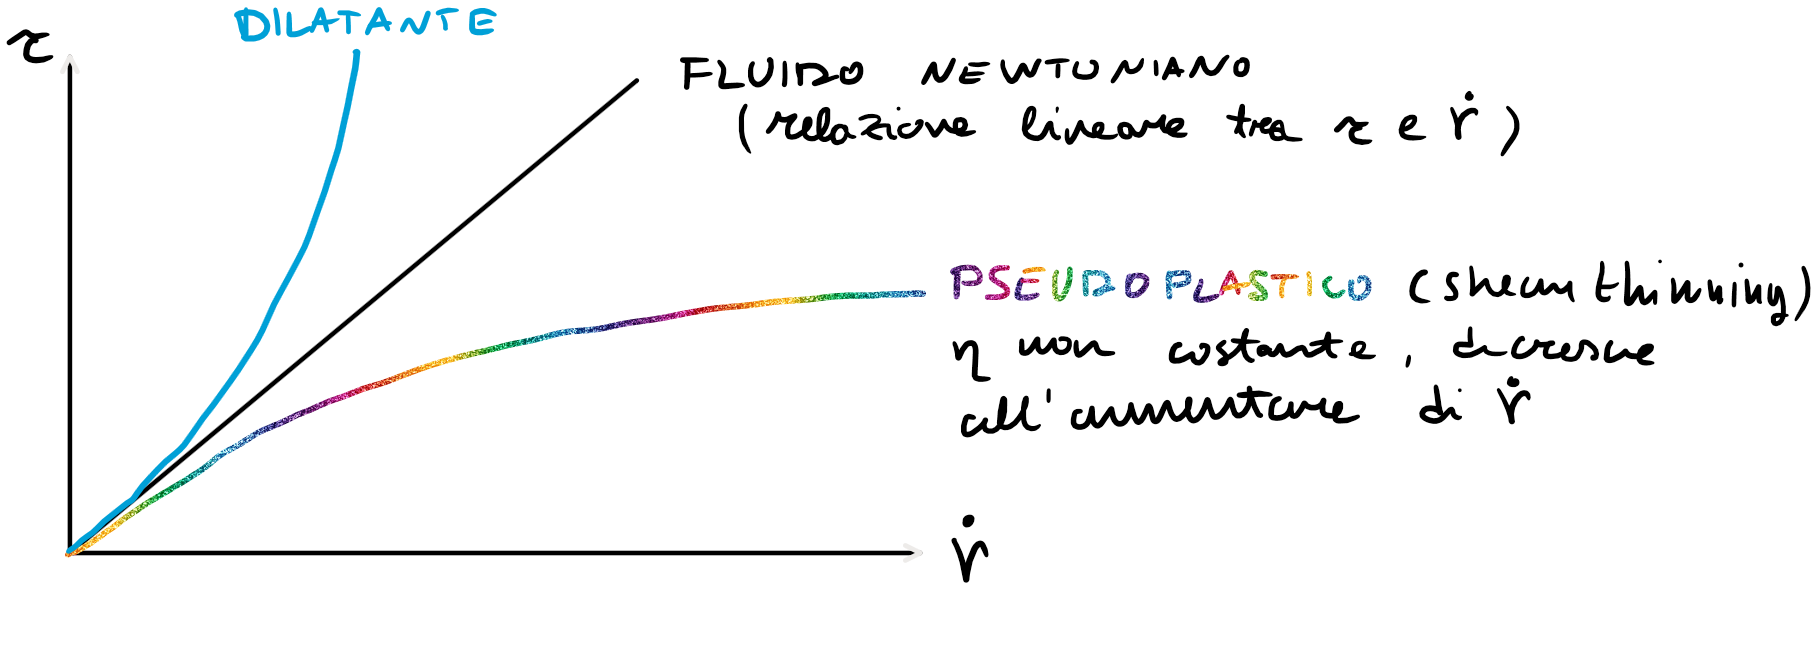
\includegraphics[width = \textwidth]{gfx/TaglioNonNewt}
\caption{Andamento dello sforzo di taglio per diversi fluidi}
\label{fig:TaglioNonNewt}
\end{figure}

Dal grafico \ref{fig:TaglioNonNewt} si può dedurre che:
all'aumentare dello sforzo di taglio il fluido si assottiglia (cioè ha comportamento \textbf{pseudo-plastico} e $\eta$ diminuisce).
Quasi tutti i materiali plastici hanno comportamento pseudo-plastico. Con $\eta$ indipendente dal tempo.
Se $\dot{\gamma}$ aumenta, significa che il fluido di assottiglia sempre di più perché viene speso molto sforzo di taglio per deformare l'oggetto. In generale viene considerato un vantaggio.

Per un fluido polimerico, si può tracciare un comportamento del tipo \ref{fig:PesudoPlastico}.
Il comportamento dilatante invece si ha per tutti i fluidi, come amidi e vernici in cui si inspessisce aumentando la velocità di deformazione.

\begin{figure}
\centering
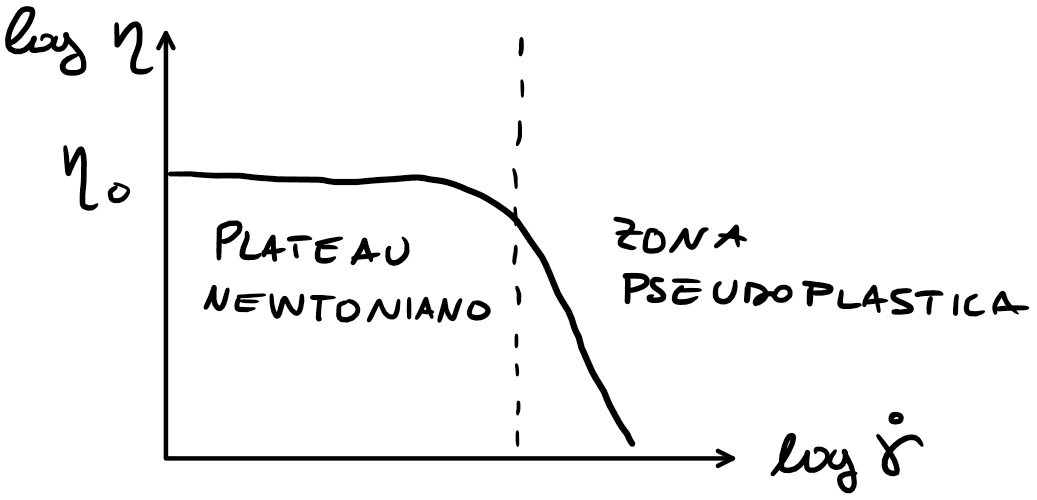
\includegraphics[width = 0.7\textwidth]{gfx/PseudoPlastico}
\caption{Comportamento di un fluido polimerico}
\label{fig:PesudoPlastico}
\end{figure}

\section{Equazioni di modellazione dei materiali polimerici}
\subsection{Legge di potenza}
Attraverso la legge di potenza si può definire:
\begin{equation}
\tau = K \lvert \dot{\gamma}^{-(n-1)}\rvert\dot{\gamma}
\label{eqn:LeggePotenza}
\end{equation}
dove:\\
\begin{tabular}{cl}
$K$ & coefficiente di consistenza\\
$n$ & indice di pseudo-plasticità
\end{tabular}\\
Il modello appena descritto dalla \eqref{eqn:LeggePotenza}, va bene per materiali pseudo-plastici e dilatanti, d'altronde basta modificare $n$ per ottenere il comportamento corretto.
\begin{description}
\item[$n\geq 1$] descrive il comportamento dei fluidi dilatanti.
\item[$n \approx 1$] descrive il comportamento dei fluidi newtoniani.
\item[$n \leq 1$] descrive il comportamento dei fluidi pseudo-plastici.
\end{description}

In generale i materiali polimerici presentano un indice di pseudo-plasticità:
$0.4 \leq n \leq 0.9$ ad eccezione del \ac{PVC} che presenta $n \approx 0.2$.

Se il materiale è caratterizzato da $n < 0.4$ in genere è indice che il modello adottato non è perfettamente adatto.
Si possono nascondere degli snervamenti che alzerebbero $n$.
Lo snervamento è difficile da misurare per cui è difficile descriverlo analiticamente.
Per osservarlo bisognerebbe imporre $\dot{\gamma}$ molto basse. Però sarebbero necessari degli strumenti molto particolare ed accurati.

Se $\dot{\gamma} > 0$ allora $\eta = K \dot{\gamma}^{n-1}$
Da cui:
\begin{equation}
\begin{split}
\log \eta &= \log\left( K \dot{\gamma}^{n-1}\right)\\
&= \log K + (n-1)\log \dot{\gamma}
\end{split}
\end{equation}
Se $0\leq n \leq 1$: la legge di potenza è semplificazione perché manca il plateau newtoniano. Funziona, come approssimazione, per lo stampaggio ad iniezione in cui si hanno velocità di deformazione che sta nel range utile della legge di potenza.

Con l'estrusione si lavora a velocità di deformazione più basse, per cui serve un modello più accurato.

\subsection{Modello di Carreau-Yasuda}
\begin{equation}
\frac{\eta - \eta_{\infty}}{\eta_0 - \eta_{\infty}} = \left[1 + (\lambda \gamma)^a\right]^{\frac{n-1}{a}}
\label{eqn:CarreauYasuda}
\end{equation}
dove:\\
\begin{tabular}{cp{0.8\textwidth}}
$\eta_0$ & Primo plateau newtoniano\\
$\eta_{\infty}$ & Secondo plateau newtoniano\\
$\lambda$ & parametro che sposta l'inclinazione del ginocchio tra plateau newtoniano e comportamento pseudo-plastico\\
$n$ & Indice di pseudo-plasticità\\
$a$ & Indice che modifica i nasi della curva. Se $n=2$ è il modello di Carreau
\end{tabular}\\

\subsection{Modello di Cross}
\begin{equation}
\eta = \eta_{\infty} + \frac{\eta_0 - \eta_{\infty}}{1+(\lambda \dot{\gamma})^n}
\end{equation}

la scelta del modello dipende dall'applicazione per cui si sta studiando il fluido, per cui i parametri si adeguano meglio.

\section{Effetti di sforzo normale e viscoelasticità}
\subsection{Sforzo normale}
Se al fluido, all'interno di un qualsiasi contenitore, viene applicato uno sforzo esterno, questo risale grazie ad un movimento di rotazione circonferenziale provocato dall'aderenza.
A livello circonferenziale, le catene polimeriche sono sollecitate a trazione. Tuttavia, nel corso del tempo esse tenderanno a ritornare allo stadio iniziale di gomitolo statistico, esercitando una pressione sull'elemento rotante. Creando così aderenza.
Questo viene anche chiamato \textbf{effetto Poisson}.

\subsection{Viscoelasticità}
Viene detto \textbf{effetto Barus} o di \textbf{rigonfiamento dell'estruso}.
Vengono rappresentati nei grafici \ref{fig:RigonfiamentoEstruso}.

\begin{figure}
\centering
\subfloat[][\emph{Effetto di rigonfiamento dell'estruso}\label{fig:Barus}]
{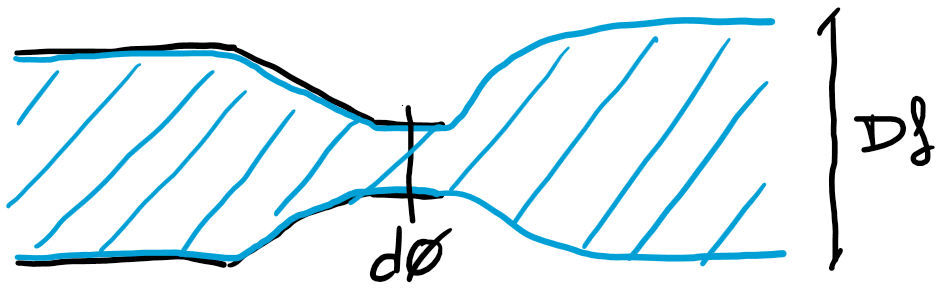
\includegraphics[width = 0.4\textwidth]{gfx/Barus}}\quad
\subfloat[][\emph{Comportamento per fluidi con effeto di rigonfiamento a diverso comportamento elastico}\label{fig:Elasticità}]
{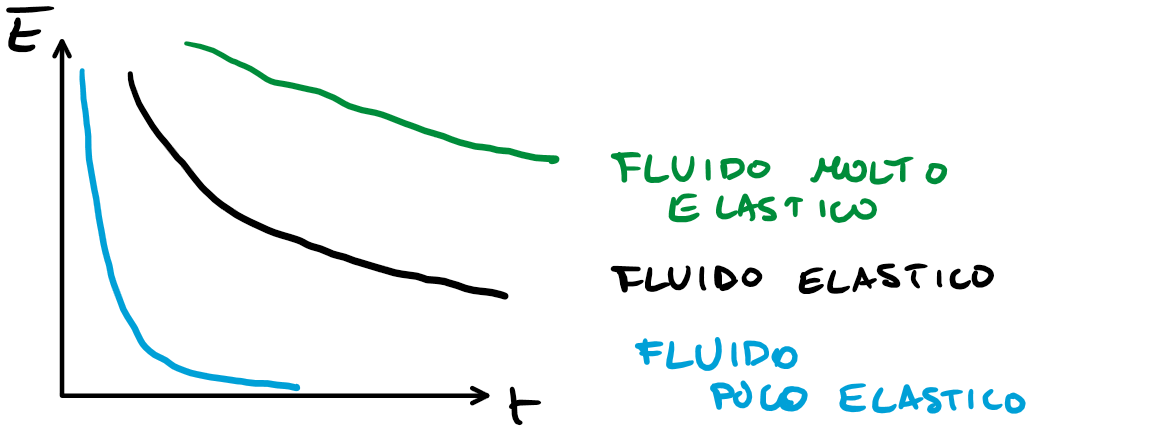
\includegraphics[width = 0.4\textwidth]{gfx/Elasticità}}
\caption{Comportamento dei fluidi con effetto di rigonfiamento dell'estruso}
\label{fig:RigonfiamentoEstruso}
\end{figure}

Si definisce che l'effetto di rigonfiamento:
\begin{equation}
De = \frac{\tau_r}{\tau_p} = \frac{\text{Tempo di rilassamento}}{\text{Tempo caratteristico del processo}}
\end{equation}
Da cui ne deriva:
\begin{description}
\item[$\tau_r \ll \tau_p$] allora $De \approx 0$ allora si dice che il fluido è poco elastico. Comportamento evidenziato al grafico \ref{fig:Elasticità}.
\item[$\tau_r \approx \tau_p$] allora $De \approx 1$ allora si dice che il fluido è più elastico. Sempre evidenziato al grafico \ref{fig:Elasticità}.
\end{description}

\section{Effetti di plasticità}
Un fluido pseudo-plastico possiede forze interne (intermolecolari) che che gli conferiscono il moto al di sotto di un certo valore $\tau$, il fluido non muoverà fino a quando tale valore non verrà superato (Comportamento del fluido di \textbf{Bingham}). 
Sotto lo \eng{Yield stress} il fluido si comporta come solido.
Sopra lo \eng{Yield stress}, lo sforzo cresce con $\dot{\gamma}$.

Il grafico \ref{fig:EffettoPlastico} rappresenta i comportamenti di un fluido puramente pseudo-plastico e il fluido di Bingham.
Entrambi hanno una legge del tipo:
\begin{description}
\item[Fluido di Bingham] $\tau = \tau_y + \eta \dot{\gamma}$
\item[Fluido pseudo-plastico] $\tau = \eta \dot{\gamma}$
\end{description}

\begin{figure}
\centering
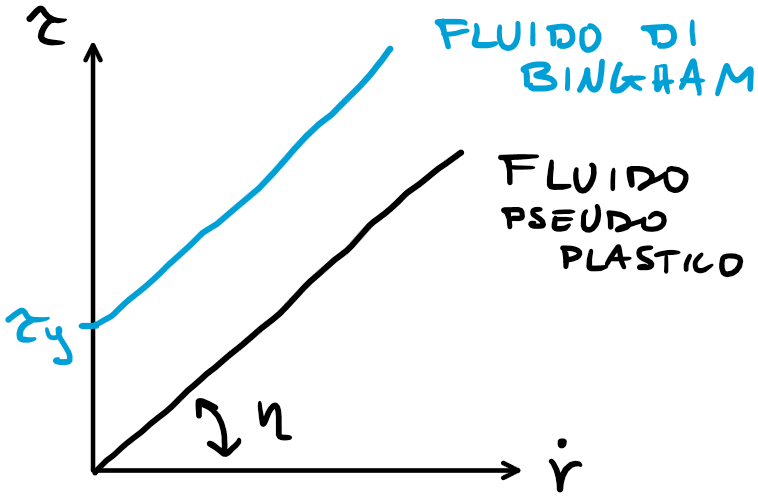
\includegraphics[width = 0.6\textwidth]{gfx/EffettoPlastico}
\caption{Rappresentazione del comportamento sotto l'effetto plastico}
\label{fig:EffettoPlastico}
\end{figure}

\section{Tissotropia}
\begin{figure}
\centering
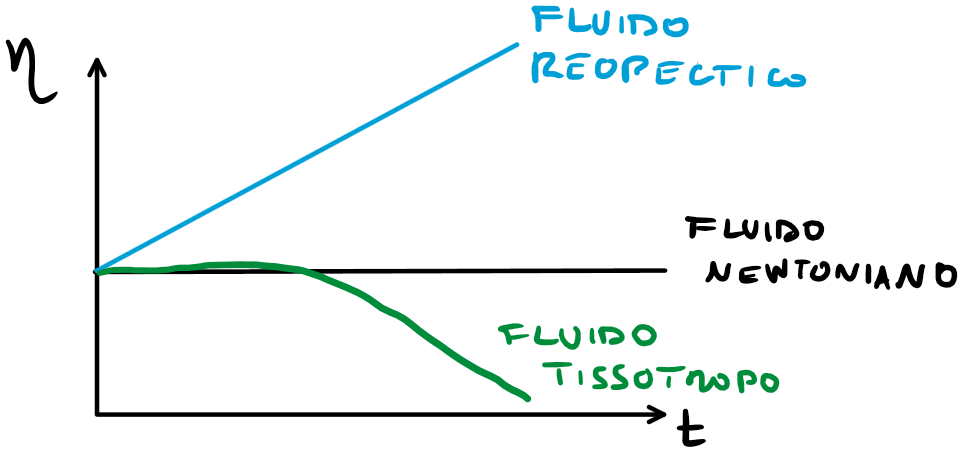
\includegraphics[width = 0.7\textwidth]{gfx/Tissotropia}
\caption{Caratteristica della viscosità in funzione del tempo}
\label{fig:Tissotropia}
\end{figure}
La tissotropia si può presentare in due forme particolari:
\begin{description}
\item[Fluido reopectico] sono quei (pochi) fluidi che aumentano la loro viscosità all'aumentare del tempo.
\item[Fluido tissotropico] sono i fluidi, non newtoniani che diminuiscono la loro viscosità all'aumentare del tempo.
\end{description}

\section{Flusso di un fluido non newtoniano}
\begin{figure}
\centering
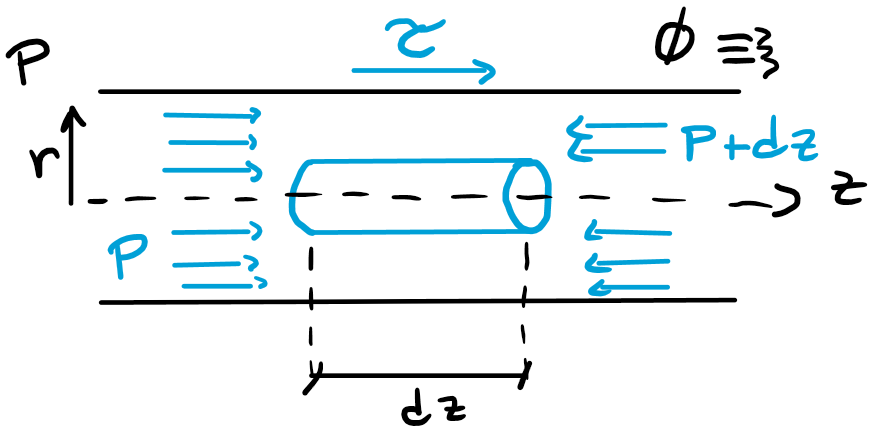
\includegraphics[width = \textwidth]{gfx/FlussoTubo}
\caption{Schematizzazione del flusso di un fluido al interno di un tubo rigido}
\label{fig:FlussoTubo}
\end{figure}
Considerando un tubo a pareti rigide come quello del disegno \ref{fig:FlussoTubo}.
Possiamo considerare le seguenti ipotesi:
\begin{itemize}
\item Il flusso è un componente simmetrico
\item Velocità del fluido indipendente da $\theta$: $dv/d\theta = 0$
\item Velocità puramente in direzione assiale: $\vec{v} = v_z \vec{e}_z$
\item Flusso completamente sviluppato $v_z = v_z(r)$
\item Accelerazione trascurabile
\end{itemize}
Allora si può scrivere l'equazione di equilibrio in z:
\begin{equation}
p \pi r^2 - (p - dp)\pi r^2 + \tau \cdot 2\pi r dz = 0
\end{equation}
Con:
\begin{equation}
\tau = \frac{dp}{dz}\frac{r}{2} \qquad \frac{dp}{dz}= cost.
\end{equation}
Se il fluido fosse newtoniano allora: $\tau = \eta \dot{\gamma}$ con $\eta = cost.$
Per un fluido non newtoniano: $\dot{\gamma} = \frac{dv}{dr} \Rightarrow \dot{\gamma}=\dot{\gamma}(r)$.
Dunque:
\begin{equation}
\begin{split}
\tau &= \frac{dp}{dz} \frac{r}{2}\\
0 &= \frac{d\tau}{dz} = \frac{d}{dz}\left(\frac{dp}{dz}\frac{r}{2}\right) =\\
&= \frac{r}{2}\underbrace{\frac{d^2p}{dz^2}}_{\frac{dp}{dz} = cost.} = 0 
\end{split} 
\end{equation}
Dunque, imponendo $p$ e assumendo che $l$ sia la lunghezza del tubo, possiamo ricavare $\tau$:
\begin{equation}
\frac{dp}{dz} = -\frac{p}{l} \qquad \tau = -\frac{p}{l}\frac{r}{2}
\end{equation}
da cui, imponendo $r = R$ ovvero il raggio del tubo:
\begin{equation}
\tau_W = -\frac{p}{l}\frac{R}{2} \Rightarrow \tau = -\tau_W \frac{r}{R}
\end{equation}
Dalla velocità di deformazione:
\begin{equation}
\dot{\gamma} = \frac{dv}{dr} \qquad \dot{\gamma} = \frac{\tau}{\eta}
\end{equation}
Allora:
\begin{equation}
\dot{\gamma} = \frac{dv}{dr} = \frac{\tau}{\eta} = -\frac{1}{\eta}\frac{p}{2l}r
\end{equation}
Si deve risolvere un sistema differenziali del primo ordine a variabili separabili:
\begin{equation}
\begin{cases}
\frac{dv}{dr} = -\frac{1}{\eta}\frac{p}{2l}r\\
v(R) = 0 :=\text{ condizione di aderenza}
\end{cases}
\end{equation}
Allora la soluzione sarà:
\begin{equation}
\begin{split}
v &= -\frac{1}{\eta}\frac{P}{2l}\frac{r^2}{2} + C \Rightarrow\\
&\Rightarrow C = \frac{1}{\eta}\frac{p}{2l}\frac{R^2}{2}\\
v &= -\frac{1}{\eta}\frac{p}{2l}\frac{r^2}{2} + \frac{1}{\eta}\frac{p}{2l}\frac{R^2}{2}\\
&= \frac{1}{\eta}\frac{p}{2l}\left(\frac{R^2}{2} - \frac{r^2}{2}\right)=\\
&=\frac{1}{\eta}\frac{p}{4l}\left(R^2 - r^2\right)
\end{split}
\end{equation}
Calcoliamo ora la portata del fluido $Q$:
\begin{equation}
\begin{split}
Q &= \int_A{v(r)\,dA} = \int_0^r{v(r) \cdot 2\pi r \, dr}=\\
&= \int_0^r{\frac{1}{\eta}\frac{p}{4l}\left(R^2 - r^2\right)\cdot 2\pi r \, dr} =\\
&= \int_0^r{2\pi \frac{p}{4\eta l} r (R^2 - r^2) \, dr} =\\
&= \frac{\pi}{2\eta} \frac{p}{l}\left[R^2 \cdot \frac{r^2}{2} - \frac{r^4}{4}\right]_0^r =\\
&=\frac{\pi}{2\eta} \frac{p}{l} \left[\frac{R^4}{2} - \frac{R^4}{4}\right] =\\
&= \frac{\pi}{8}\frac{R^4}{l}\left(\frac{1}{\eta}\right)(p)
\end{split}
\end{equation}
Dove il termine $\frac{R^4}{l}$ descrive la dipendenza della portata dalla geometria del tubo, risulta essere il termine preponderante nell'equazione.
Mentre, il termine $\frac{1}{\eta}$ mostra la dipendenza della portata dal comportamento viscoso del fluido.

Applichiamo ora la legge di potenza, che descrive il comportamento della maggior parte dei fluidi.
\begin{equation}
\frac{dp}{dz}=-\frac{p}{l} \qquad \tau = -\frac{p}{l}\frac{r}{2}
\end{equation}
Ricordando che:
\begin{equation}
\tau = \eta \dot{\gamma} \qquad \tau = K \lvert \dot{\gamma} \rvert^{n-1}\dot{\gamma}
\end{equation}
Sostituendo:
\begin{equation}
\underbrace{K \Big|\frac{dv}{dr}\Big|^{n-1}\frac{dv}{dr}}_{\tau} = -\frac{p}{l}\frac{r}{2}
\end{equation}
Tra l'altro vale che: se $\tau \leq 0$ allora $\frac{dv}{dr} \leq 0$.
\begin{equation}
\begin{split}
K \left(-\frac{dv}{dr}\right)^{n-1}\left(-\frac{dv}{dr}\right) &= \frac{p}{l}\frac{r}{2}\\
K \left(-\frac{dv}{dr}\right)^{n} &= \frac{p}{l}\frac{r}{2} 
\end{split}
\end{equation}
Allora, si può scrivere un sistema differenziale a variabili separabili.
\begin{equation}
\begin{cases}
\frac{dv}{dr}=-\left(\frac{p}{2Kl}\right)^{1/n}r^{1/n}\\
v(R) = 0 \quad \text{Aderenza a parete}
\end{cases}
\end{equation}
Da cui
\begin{equation}
v(r) = -\left(\frac{p}{2Kl}\right)^{1/n}\frac{r^{\frac{1}{n}+1}}{\frac{1}{n}+1}+C
\end{equation}
Da cui imponendo la condizione iniziale si ottiene
\begin{equation}
v(r) = \left(\frac{p}{2Kl}\right)^{1/n} \frac{n}{1+n} \left(R^{\frac{1}{n}+1} - r^{\frac{1}{n}+1}\right)
\end{equation}
Sostituendo con $n=1$ si dovrebbe riottenere la legge per il fluido newtoniano.
Alla figura \ref{fig:SpeedProfile}, sono rappresentati i principali profili di velocità per fluidi descrivibili tramite legge di potenza.

\begin{figure}
\centering
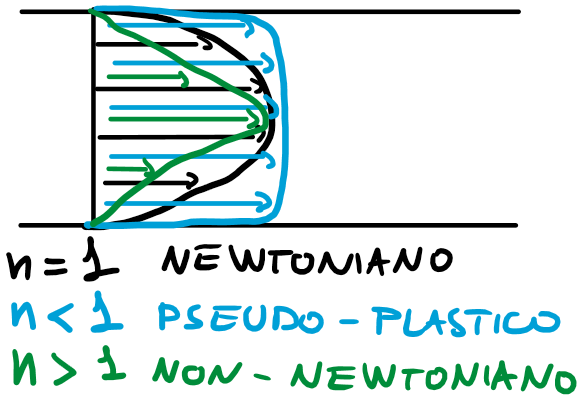
\includegraphics[width = \textwidth]{gfx/SpeedProfile}
\caption{Profili di velocità per diversi fluidi}
\label{fig:SpeedProfile}
\end{figure}

Calcoliamo la portata del fluido nel caso del tubo.
\begin{equation}
\begin{split}
Q &= \int_A{v(r)\,dA} = 2\pi \int_0^r{v(r)\,dr}\\
&= \int_0^r{\left(\frac{p}{2Kl}\right)^{1/n} \frac{n}{1+n} \left(R^{\frac{1}{n}+1} - r^{\frac{1}{n}+1}\right) r\,dr}=\\
&= 2\pi \left(\frac{p}{2Kl}\right)^{\frac{1}{n}}\frac{n}{n+1}\left[R^{1+\frac{1}{n}}\frac{r^2}{2} - \frac{r^{3+\frac{1}{n}}}{3 + \frac{1}{n}}\right]_0^r=\\
&= 2\pi \left(\frac{p}{2Kl}\right)^{1/n}\frac{n}{n+1}\left[\frac{R^{3+\frac{1}{n}}}{2} - \frac{R^{3+\frac{1}{n}}}{3+\frac{1}{n}}\right]=\\
&= 2\pi \left(\frac{p}{2Kl}\right)^{1/n}\frac{n}{n+1} R^{3+\frac{1}{n}} \frac{3+\frac{1}{n} -2}{2\left(3+\frac{1}{n}\right)} =\\
&=\pi \left(\frac{p}{2Kl}\right)^{1/n} \frac{n}{n+1} R^{3+\frac{1}{n}} \frac{1+\frac{1}{n}}{3+\frac{1}{n}} =\\
&=\frac{\pi}{2^{1/n}} \left(\frac{1}{K}\right)^{1/n} \frac{n}{3n+1} \frac{R^{3+\frac{1}{n}}}{l^{1/n}} p^{1/n}
\end{split}
\end{equation}
Dove:\\
\begin{tabular}{cp{0.8\textwidth}}
$\frac{\pi}{2^{1/n}} \left(\frac{1}{K}\right)^{1/n} \frac{n}{3n+1}$ & Lega la portata alla tipologia del materiale\\
$ \frac{R^{3+\frac{1}{n}}}{l^{1/n}}$ & Lega la portata alla geometria del tubo\\
$p^{1/n}$ & Lega portata e pressione
\end{tabular}

%%%%%%%%%%%%%%%%%%%%%%%%%%%%%%%%%%%%%%%%%%%%%%%%%%%%%%%%%%%%%%%%%%%%%%%%%%%%%%%
\chapter{Reologia (o Reometria)}\label{chp:Reologia}
%%%%%%%%%%%%%%%%%%%%%%%%%%%%%%%%%%%%%%%%%%%%%%%%%%%%%%%%%%%%%%%%%%%%%%%%%%%%%%%
La reologia studia la deformazione di un corpo sotto l'azione di uno sforzo.
I fluidi ideali, liquidi o gassosi che siano, si deformano irreversibilmente. L'energia di deformazione viene dissipata all'interno dei fluido sotto forma di calore, non può essere recuperata alla cessazione dello sforzo. Nella realtà non si trovano né fluidi ideali, né solidi ideali.
Solo pochi liquidi si avvicinano, come comportamento a quello dei liquidi ideali. La maggior parte dei liquidi mostrano reologiacamente un comportamento che li classifica nella regione tra i liquidi e solidi: essi sono sia elastici che viscosi e possono perciò essere definiti "viscoelastici", che possono subire solo sforzi di taglio.

La resistenza di un fluido rispetto ad ogni cambiamento irreversibile dei suoi elementi di volume viene detta viscosità.

\section{La legge della viscosità}
\subsection{La legge di Newton}
La misura della viscosità dei liquidi richiede dapprima la definizione dei parametri che riguardano il flusso. Si potranno poi trovare opportune condizioni per l'esecuzione dei test che consentono la misurazione delle grandezze in modo obbiettivo e riproducibile.
Newton fu il primo a formulare la legge fondamentale della viscometria che descrive il comportamento di flusso di un liquido ideale.
\begin{equation}
\tau = \eta \cdot \dot{\gamma}
\label{eqn:1LeggeNewton}
\end{equation}

\paragraph{Lo sforzo di taglio}
Una forza $\mathbf{F}$ applicata ad un'area $A$ (interfaccia tra il piatto superiore il liquido sottostante) provoca un movimento di scorrimento nello strato liquido. la velocità di flusso che può essere mantenuta per una data forza sarà determinata dalla resistenza interna del liquido, cioè dalla sua viscosità.
\begin{equation}
p = \frac{\mathbf{F}}{A} = \left[\frac{N}{m^2}\right] = \left[Pa\right]
\end{equation}

\section{Le curve di flusso e di viscosità}
la correlazione tra lo sforzo di taglio e gradiente di velocità che definisce il comportamento reologico di un liquido può essere graficamente riportato in un diagramma $\tau/D$. Il diagramma prende il nome di \textbf{curva di flusso}.
Altro diagramma assai comune è quello che riporta $\eta$ in funzione di $D$ (velocità). Questo diagramma è detto \textbf{Curva di viscosità}.

\section{Fluidi pseudo-plastici}
Molti liquidi mostrano una drastica diminuzione della viscosità quando il gradiente di velocità passa da bassi valori ad alti. In altre parole: quanto più veloce i prodotti farmaceutici vengono spinti, attraverso tubi, o capillari, quanto più velocemente i le vernici vengono spruzzate o pennellate, tanto più diminuisce la viscosità di questi materiali.
Tecnicamente questo significa che sotto l'azione di una determinata forza (o pressione) una maggiore quantità di materiale può essere soggetta allo scorrimento o che può essere ridotto il lavoro meccanico necessario a mantenere una determinata portata.
I materiali che subiscono una fluidificazione dovuta all'aumento del gradiente di velocità sono detti \textbf{pseudo-plastici}.
All'aumentare del gradiente di velocità le particelle allungate sospese nel liquido si orientano nella direzione del moto. Le macromolecole di un fuso o di una soluzione possono disintecciarsi, allungarsi e orientarsi parallelamente alla direzione della forza impressa. L'allineamento delle particelle o delle molecole consente loro di scivolare le une sulle altre e questo comporta una diminuzione della viscosità.
Per la maggior parte dei liquidi la diminuzione di $\eta$ al crescere di $D$ è irreversibile, magari dopo un certo lasso di tempo, cioè il liquido riacquista la sua elevata viscosità originale per cessazione dello sforzo applicato.


%%%%%%%%%%%%%%%%%%%%%%%%%%%%%%%%%%%%%%%%%%%%%%%%%%%%%%%%%%%%%%%%%%%%%%%%%%%%%%%
\chapter{Misure di Viscosità}\label{chp:MisureViscosità}
%%%%%%%%%%%%%%%%%%%%%%%%%%%%%%%%%%%%%%%%%%%%%%%%%%%%%%%%%%%%%%%%%%%%%%%%%%%%%%%
\section{Viscosimetri rotazionali}
Il principio di funzionamento dei viscosimetri rotazionali con sistema di misura a cilindri coassiali o a piatto cono consente la progettazione di viscosimetri assoluti estremamente versatili.
Nel mercato se ne trovano molti, di vari modelli con alta varietà di prezzo.
Si può pensare al sistema di misura a cilindri coassiali per i viscosimetri rotazionali come derivante dal modello a piatti paralleli di Newton, con la semplice incurvatura dei piatti in due cilindri, l'uno al interno dell'altro. Il campione di liquido riempe l'intercapedine anulare (in visosimetria molto spesso indicata come \eng{gap}) tra i due cilindri può essere sottoposto a taglio. Il moto deve essere laminare al fine di consentire la trattazione matematica del problema.
Si può:
\begin{itemize}
\item Fissare $\tau$ e valutare $D(\dot{\gamma})$: Il cilindro interno, o esterno, impone un definito sforzo di taglio (o momento torcente) mentre l'altro è fermo.
Si può misurare la velocità di rotazione o il gradiente di velocità risultante. Si basano su questo principio i viscosimetri tipo \eng{Krebs-Stormer}.
\item Fissare $\dot{\gamma}$ e trovare $\tau$.
Uno dei cilindro ruota a velocità costante, mentre l'altro è fermo. Si può misurare lo sforzo di taglio risultante o il momento torcente. La maggior parte dei viscosimetri in commercio sfruttano tale principio.
\end{itemize}

\section{Viscosimetro di Couette}
In questo tipo, il cilindro ruota a velocità prefissata mentre la coppia viene misurata da quello interno, attraverso un elemento simile a quello descritto precedentemente (ad esempio una molla).
I viscosimetri di \eng{Couette} sono più stabili di quelli \eng{Searie} per quanto riguarda le forze centrifughe. naturalmente le misure fatte con viscosimetri di tipo diverso danno gli stessi valori di viscosità assoluta per uno stesso fluido.
Se i due viscosimetri sono equipaggiati con ciclindri coassiali di raggio poco diverso, cioè se l'intercapedine in cui sta il fluido è molto sottile, il gradiente $D$ è costante all'interno del fluido, così la viscosità del fluido stesso.
\begin{equation}
\dot{\gamma} = \frac{dv}{dh} = \frac{V}{H} \Rightarrow \tau = \eta \frac{V}{H}
\end{equation}
Per effettuare la misura, si inserisce un cilindro dentro l'altro. Fissato il cilindro esterno, mentre quello interno viene mosso con velocità costante.

\begin{figure}
\centering
\subfloat[][\emph{Schema viscosimetro}\label{fig:Viscosimetro}]
{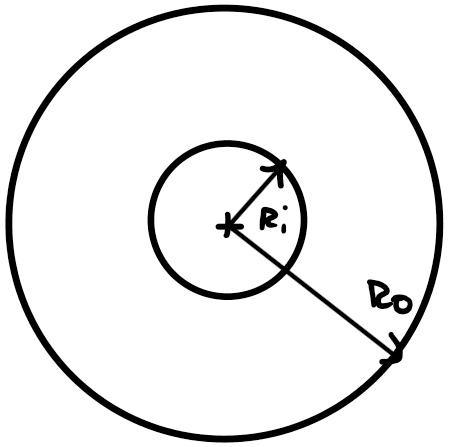
\includegraphics[width = 0.4\textwidth]{gfx/Viscosimetro}}\quad
\subfloat[][\emph{Relazioni calcolate dal viscosimetro}\label{txt:Viscosimetro}]{
\begin{minipage}[b]{0.4\textwidth}
\begin{align*}
H &= R_o - R_i\\
V &= \omega R_i\\
\dot{\gamma} &= \frac{V}{H} = \frac{\omega R_i}{R_o - R_i}\\
\end{align*}
Per ottenere $\tau$ devo trovare il momento torcente:
\begin{align*}
M_{torc} &= \tau 2\pi R_i \cdot \underbrace{l \cdot r_i}_{\text{azione di }\tau} =\\
&= \tau 2\pi \cdot l \cdot R_i^2\\
\Rightarrow \tau &= \frac{M_{torc}}{2\pi l R_i^2} 
\end{align*}
\end{minipage}}
\caption{Funzionamento di un viscosimetro}
\label{exp:Viscosimetro}
\end{figure}

Siccome deve valere che $\eta = \tau / \dot{\gamma}$ se si vuole $\dot{\gamma}$ elevata, bisogna muovere il cilindro interno generando forze centrifughe.
Tuttavia se si accelera troppo il fluido, esso sarà soggetto a instabilità.

\section{Reometro Piatto-Cono}
Nei sistemi di misura piatto-cono (detti \ac{PK}), il problema fondamentale risulta la pulizia.
In certi casi, la pulizia del rotore e della campana dopo aver eseguito dei test è talmente complicata da far orientare la scelta sul sistema piatto-cono, assai più facile da pulire%
\footnote{Soprattutto dopo aver fatto dei test su dei pigmenti}.
alle volte vengono eseguite delle prove su dei campioni contenenti materiali preziosi (in campo dell'elettronica) ed è fondamentale che venga recuperato tutto il campione.
In generale la quantità di campione richiesta per eseguire prove su \ac{PK} è molto inferiore rispetto al sistema a cilindri coassiali.
per la maggior parte dei \ac{PK} sono sufficienti poche gocce di liquido.
I sistemi di misura \ac{PK} trovano la loro principale applicazione nel campi degli alti gradienti di velocità.

Vi sono però alcune importanti limitazioni nell'uso dei sistemi di misura \ac{PK}:
\begin{itemize}
\item L'angolo del cono (in genere si usano angoli variabili tra $0.3\unit{\degree} \div 1.0\unit{\degree}$) fa sì che l'intercapedine tra il piatto e cono varia da zero in punta al cono al valore massimo al raggio $R_o$. Le dispersioni con particelle, anche le più piccole possibili, non sono adatte per la zona vicina alla punta del cono.
\item Le particelle vengno spinte dalla zona della punta verso l'esterno e questo può accadere prima ancora dell'inizio della prova, quando il piano viene avvicinato al cono fino al contatto. Durante la prova, si ha un flusso secondario di particelle in direzione radiale che si sovrappone al flusso principale (circolare). Influenzando negativamente il moto laminare. Una simile situazione tende a rendere ancora di più eterogenei i campioni, falsando la prova.
\item Le particelle più grandi richiedono l'uso di angoli maggiori $1\unit{\degree} \div 3\unit{\degree}$ con conseguenti maggiori effetti negativi del flusso secondario sui risultati del test.
\item I sistemi \ac{PK} sono influenzati dalle forze normali che sono il risultato della risposta elastica dei campioni viscoelastici soggetti a taglio.
Queste forze normali possono trascinare elementi di volume fuori del gap angolare e farli arrampicare sul bordo esterno del cono, In tale situazione si ha spaccamento del campione verso la metà del gap angolare. Ciò è un problema che disturba fortemente la misura.
Un'indicazione della presenza di questo inconveniente è il formarsi di una cresta sempre più grande sul bordo del cono. Spesso si arriva addirittura a vedere la spaccatura del campione guardando da vicino la rotazione del cono.
\end{itemize} 

\begin{figure}
\centering
\subfloat[][\emph{Funzionamento del cono (1), caso di separazione del campione (2)}\label{fig:PK}]
{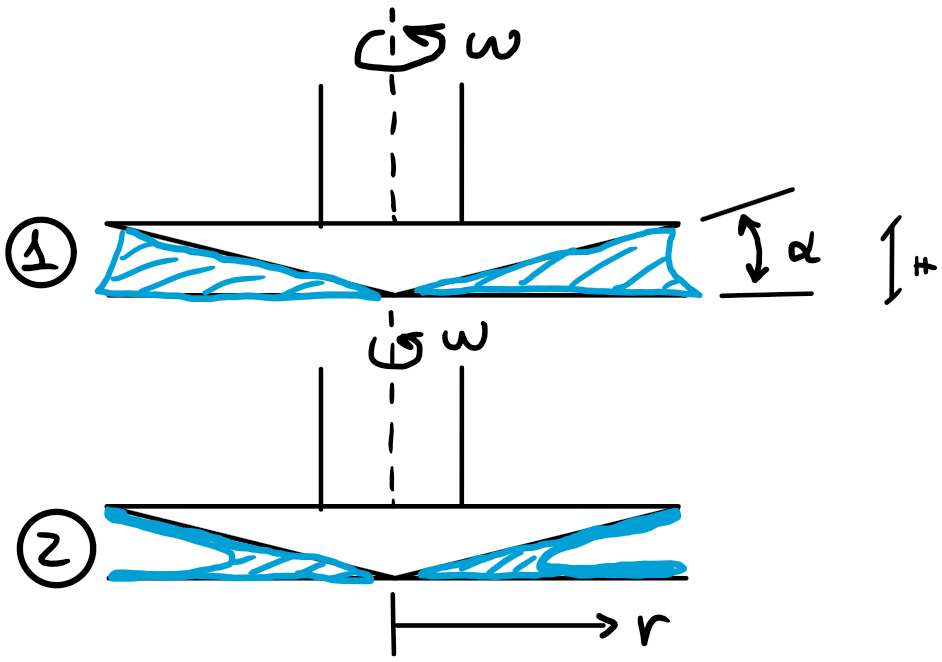
\includegraphics[width = 0.4\textwidth]{gfx/PK}}\quad
\subfloat[][\emph{Grafico ottenuto dal test}\label{fig:PK_graph}]
{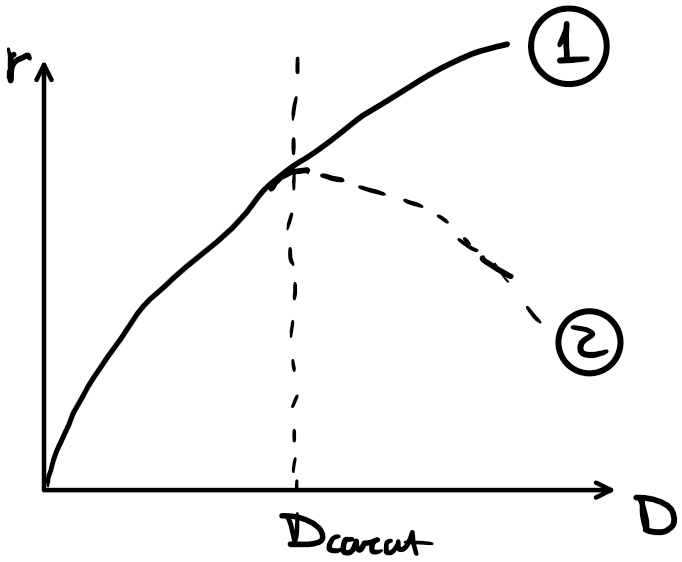
\includegraphics[width = 0.4\textwidth]{gfx/PK_graph}}
\caption{Schematizzazione dei test eseguiti tramite sistema \ac{PK}}
\label{fig:TestPK}
\end{figure}
Allora i calcoli che permettono di ottenere una valutazione della viscosità diventano:
\begin{align}
v &= \omega r \frac{z}{\alpha r}\\
&= \frac{\omega z}{\alpha}\\
\Rightarrow \dot{\gamma} &= \frac{dv}{dz} = \frac{\omega}{\alpha}\: cost.
\end{align}
Dunque:
\begin{equation}
\tau = \eta \frac{\omega}{\alpha}
\end{equation}
\begin{align}
M_t &= \int_0^R \tau 2\pi r^2 dr =\\
&= 2\pi \eta \frac{\omega}{\alpha} \frac{R^3}{3}\\
\Rightarrow \tau &= \frac{3 M_t}{2\pi R^3}
\end{align}
Da cui in fine si ottiene la viscosità sostituendo in
\begin{equation}
\eta = \frac{\tau}{\dot{\gamma}}
\end{equation}

\section{Reometro Piatto-Piatto}
\begin{figure}
\centering
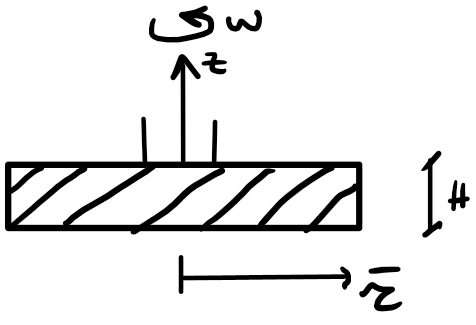
\includegraphics[width = 0.5\textwidth]{gfx/PiattoPiatto}
\caption{Schema del rotore per uno strumento piatto piatto}
\label{fig:PiattoPiatto}
\end{figure}

Nella figura \ref{fig:PiattoPiatto} viene rappresentato il rotore dello strumento per la misura della viscosità.
La relazione che ci permetterà di ottenere la viscosità sarà:
\begin{equation}
v(r,z) = \omega r \frac{z}{H} =%
\begin{cases}
\omega r & se z = H\\
0 & se z = 0
\end{cases}
\end{equation}
Da cui allora:
\begin{equation}
\dot{\gamma} = \frac{dv}{dz} = \frac{\omega r}{H}
\end{equation}
\begin{equation}
\dot{\gamma}_R = \frac{dv}{dz} = \frac{\omega R}{H}
\end{equation}
Calcoliamo il momento torcente
\begin{equation}
M_t = \int_0^R{\tau 2\pi r^2 dr}
\end{equation}
Ipotizzando che si sita analizzando un fluido newtoniano.
\begin{equation}
\eta \frac{\omega}{H} 2\pi \int_0^R{r^3 dr} =%
2\pi \eta \frac{\omega}{H} \frac{R^4}{4}
\end{equation}
Da cui
\begin{equation}
\frac{\pi}{2} \eta \frac{\omega}{H} R^4
\end{equation}
Notiamo che
\begin{equation}
\frac{\pi}{2} \underbrace{\eta \frac{\omega R}{H}}_{\tau} R^3 = \frac{\pi}{2} \tau_R R^3
\end{equation}
Invertendo l'equazione di definizione del momento torcente:
\begin{equation}
\tau_R = \frac{M_t 2}{\pi R^3}
\end{equation}
Da cui finalmente si ottiene la densità, sempre ricordando che tutti questi ragionamenti valgono per un fluido newtoniano:
\begin{equation}
\eta = \frac{\tau_R}{\dot{\gamma}_R}
\end{equation}

\section{Viscosimetro capillare}
L'utilità di questo tipo di misuratore, di fatto è la controparte del \ac{MFI}.
In quanto in termini di:
\begin{description}
\item[Pressione] \ac{MFI} controllando la pressione da cui si misura la portata di fluido;
\item[Portata di flusso] Viscosimetria capillare: si controlla la portata e si misura la pressione.
\end{description}

Il reometro è costituito da una camera cilindrica in cui viene caricato il materiale che successivamente viene estruso attraverso l'ugello. Viene spinto da un pistone che scorre verso il basso.
Il materiale viene tenuto fuso grazie ad un forno che circonda la camera, mantenendola ad una temperatura $T$ impostata.
Durante la misura, il pistone scende secondo velocità impostata e, contemporaneamente, ad intervalli prestabiliti misura il valore della forza necessaria all'estrusione del materiale.
La misura avviene grazie ad una cella di carico che lavora in un range $0 \div 2000\unit{\N}$, alloggiata nella testa del pistone.
Al fine di determinare le relazioni che legano: lo sforzo di taglio, il gradiente di velocità e le grandezze misurabili nel sistema, è necessario studiare il flusso in un capillare.
Partendo dalla figura \ref{fig:Capillare}, si può scrivere il bilancio delle forze sul cilindro di fluido di raggio $R$ e lunghezza $L$
\begin{equation}
(P_1 - P_2)\pi R^2 = 2\pi RL \tau_W
\end{equation}
da cui
\begin{equation}
\tau_W = \frac{\Delta P R}{2 L}
\end{equation}

\begin{figure}
\centering
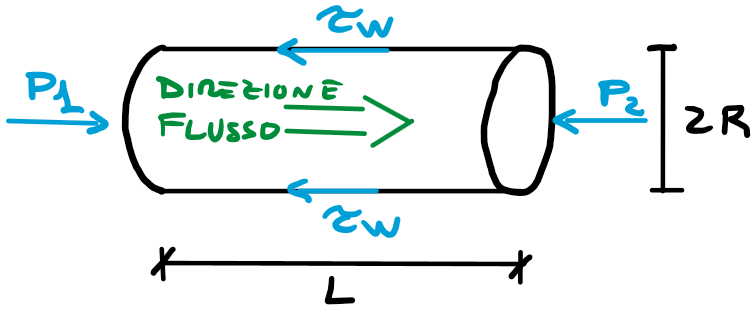
\includegraphics[width = \textwidth]{gfx/Capillare}
\caption{Indicazioni dei parametri del sistema per la misura capillare}
\label{fig:Capillare}
\end{figure}

Nel caso che il bilancio venga scritto in corrispondenza di un raggio generico, si avrebbe:
\begin{equation}
\tau = \frac{\Delta P r}{2 L}
\end{equation}

Per poter determinare le relazioni tra le varie grandezze, l'approccio conveniente è quello di introdurre un'equazione costitutiva semplice%
\footnote{Ad esempio quella dei fluidi newtoniani.}
cercando poi una correzione che permetta di estendere le equazioni trovate a qualunque tipo di fluido.

Introduciamo l'equazione costitutiva relativa ad un fluido newtoniano sostituendola allo sforzo di taglio:
\begin{equation}
\eta \frac{d V_z}{dr} = \frac{\Delta P r}{2 L}
\end{equation}
questa equazione differenziale a variabili separabili ci permette di determinare l'espressione del profilo di velocità in funzione del ragio. Separando le variabili e considerando che in $V_z(R) = 0$:
\begin{equation}
\int_0^{V_z(r)}{\frac{2\eta L}{\Delta P} dV_z} = \int_R^r rdr
\end{equation}
da cui:
\begin{equation}
V_z(r) = \frac{\Delta P}{4 \eta L} R^2 \left[1 - \left(\frac{r}{R}\right)^2\right] 
\end{equation}

La portata $Q$ può essere ottenuta integrando il profilo di velocità sull'area della sezione di passaggio è data da:
\begin{equation}
Q = \frac{\Delta P \pi R^4}{8 \eta L} \Leftarrow%
\frac{\pi R^3}{4 \eta} \tau_{\omega} =%
\frac{\pi R^3}{4 \eta} \frac{\overbrace{P R}^{\tau_{\omega}}}{2L}
\end{equation}

Dall'equazione dello sforzo di taglio alla parete $\tau_W$ è possibile calcolare lo sforzo di taglio alla parete:
\begin{equation}
\dot{\gamma}_W = \frac{\tau_W}{\eta} = \frac{\Delta P R}{2 L}
\end{equation}
Sostituendo in questa, l'equazione di $\Delta P$ ricavabile dalla definizione della portata:
\begin{equation}
\dot{\gamma}_W = \frac{4Q}{\pi R^3}
\end{equation}
Quando il fluido ha comportamento non newtoniano, è necessario introdurre due correzioni:
\begin{enumerate}
\item Correzione di Rabinowitsch;
\item Correzione di Bagley.
\end{enumerate}

\paragraph{Melt Flow Index}
Riprendendo ciò che era già stato visto al capitolo dedicato.
%TODO aggiungere il riferimento al capitolo\eng{•}

\begin{equation}
\text{Portata} = \frac{\text{Pressione}}{A}
\end{equation}
con:
\begin{equation}
A = \frac{\pi D^2}{4}
\end{equation}
Si considera allora:
\begin{description}
\item[MFI alto] allora $\mu \downarrow$ con circa
$MFI \approx 25 \div 50 \unit{\g/10\min}$
\item[MFI basso] allora $\mu \uparrow$ con circa
$MFI \approx 0.5 \div 5 \unit{\g/10\min}$
\end{description}

\begin{figure}
\centering
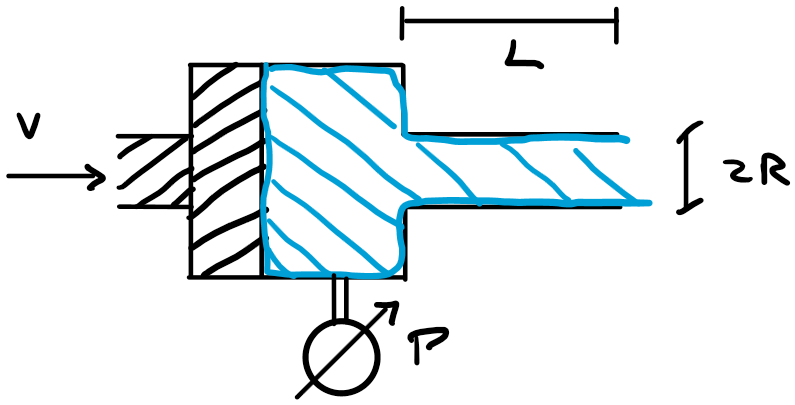
\includegraphics[width = 0.5\textwidth]{gfx/CorrezioneCapillare}
\caption{Descrizione del viscosimetro capillare con le correzioni per i fluidi non newtoniani}\label{fig:CorrezioneCapillare}
\end{figure}

\subsection{Correzione di Rabinowitsch}
\begin{equation}
\dot{\gamma}_W = \frac{4 Q}{\pi R^3} + \ldots
\end{equation}

\subsection{Correzione di Mooney}
Corregge lo scorrimento per adesione alle pareti che non veniva considerato nella correzione di Rabinowitsch.
Per eseguire più velocemente nell'esecuzione della prova si può usare un lubrificante. Saranno però necessarie più misure per raggi diversi.
Allora:
\begin{equation}
\dot{\gamma}_W  = \frac{4 Q}{\pi R^3} = \dot{\gamma}_N
\end{equation}
Sapendo che:
\begin{equation}
\dot{\gamma} = \frac{dv}{dr} \quad \dot{\gamma}_W = \frac{dv}{dr}\Big|_{r = R}
\end{equation}
Dal moto di Poiseville si può descrivere:
\begin{equation}
\tau = - \frac{r}{R}\tau_W \quad \tau_W = \frac{PR}{2L}
\end{equation}
allora si può andare a definire la portata per la figura \ref{fig:CorrezioneCapillare}:
\begin{equation}
\begin{split}
Q &= \int_A{v(r) dA} = \int_0^R{v(r) \underbrace{2\pi r dr}_{dA}} = 2\pi \int_0^R{v(r) r dr} =\\
&= 2\pi \left[v(r) \frac{r^2}{2}\right]_0^R - \int_0^R{\frac{dv}{dr}\frac{r^2}{2}dr} =\\
&= 2\pi \left[v(R)\frac{R^2}{2} - v(0)\frac{0^2}{2}\right] - \int_0^R{\dot{\gamma}\frac{r^2}{2}dr} =\\
&= -\pi \int_0^R{\dot{\gamma}r^2 dr} \Rightarrow \underbrace{\left[r = \frac{\tau}{\tau_W}R\right]}_{\text{cambio variabili}} \Rightarrow\\
&\Rightarrow \pi \int_{0 \mid r = 0}^{-\tau_W \mid r=R \Rightarrow \tau = -\tau_W}{\dot{\gamma}(\tau)\frac{\tau^2}{\tau_W^2}R^2\frac{R}{\tau_W}d\tau}=\\
&= \pi \frac{R^3}{\tau_W^3}\int_0^{-\tau_W}{\dot{\gamma}(\tau) \tau^2 d\tau}
\end{split}
\end{equation}
Da cui
\begin{equation}
\begin{split}
\frac{dQ}{d\tau_W} &= -\frac{3}{\tau_W^4}\pi R^3%
\int_0^{-\tau_W}{\dot{\gamma}(\tau)\tau^2 d\tau} - \frac{\pi R^3}{\tau_W^3} \dot{\gamma}(-\tau_W)\tau_W^3\\
&= -\frac{3\pi R^3}{\tau_W^4}\int_0^{-\tau_W}{\dot{\gamma}\tau^2 d\tau} + \frac{\pi R^3}{\tau_W}\dot{\gamma}_W
\end{split}
\end{equation}
Per cui:
\begin{equation}
Q = \frac{\pi R^3}{\tau_W^3}\int_0^{-\tau_W}{\dot{\gamma}(\tau)\tau^2 d\tau}
\end{equation}
Svolgendo l'integrale si arriva ad ottenere:
\begin{equation}
\frac{Q \tau_W^3}{\pi R^3}
\end{equation}
Allora:
\begin{equation}
\begin{split}
\frac{dQ}{d\tau_W} &= - \frac{3\pi R^3}{\tau_W^4} \frac{Q \tau_W^3}{\pi R^3} + \frac{\pi R^3}{\tau_w}\dot{\gamma}_W\\
\frac{dQ}{d\tau_w} &= -\frac{3Q}{\tau_W} + \frac{\pi R^3}{\tau_W}\dot{\gamma}_W
\end{split}
\end{equation}
Imponiamo la pre-moltiplicazione per $4/\pi R^3$ :
\begin{equation}
\frac{4}{\pi R^3}\frac{dQ}{d\tau_w} = \left[-\frac{3Q}{\tau_W}+\frac{\pi R^3}{\tau_w}\dot{\gamma}_W\right]\frac{4}{\pi R^3}
\end{equation}
Inoltre
\begin{equation}
\frac{\dot{\gamma}_W}{d\tau_W} = -\frac{3 Q \dot{\gamma}_N}{\tau_W} + \frac{4 \dot{\gamma}_W}{\tau_W}
\end{equation}
Da cui:
\begin{equation}
\begin{split}
\dot{\gamma}_W &= \frac{\tau_W}{4}\left[\frac{3}{\tau_W}\dot{\gamma}_W + \frac{d\dot{\gamma}_W}{d\tau_W}\right]\\
\dot{\gamma}_W &= \gamma_W \left[\frac{3}{4} + \frac{1}{4}\frac{\tau_W}{\dot{\gamma}_N}\frac{d\dot{\gamma}_N}{d\tau_W}\right]
\end{split}
\end{equation}
Piccola nota sull'ultimo termine dell'equazione precedente:
\begin{equation}
\frac{\tau_W}{\dot{\gamma}_N} \frac{d\dot{\gamma}_N}{d\tau_W} = \frac{\frac{d\dot{\gamma}_N}{\dot{\gamma}_N}}{\frac{d\tau_W}{\tau_W}} = \frac{d \ln\dot{\gamma}_N}{d\ln\tau_W}
\end{equation}
Dunque:
\begin{equation}
\dot{\gamma}_W = \dot{\gamma}_N\left[\frac{3}{4} + \frac{1}{4} \frac{d \ln\dot{\gamma}_N}{d\ln\tau_W}\right]
\end{equation}
Seguendo la \textbf{legge di potenza} si può scrivere:
\begin{equation}
\frac{d \ln\dot{\gamma}_N}{d\ln\tau_W} = \frac{1}{n} \Rightarrow \text{Fattore di Rabinowitch} \Rightarrow \frac{3n+1}{4n}
\end{equation}
In fine:
\begin{equation}
\dot{\gamma_W} = \frac{4Q}{\pi R^3}\frac{3n+1}{4n}
\end{equation}
Per definire correttamente il rapporto $\frac{d \ln\dot{\gamma}_N}{d\ln\tau_W}$ si può ottenere in maniera sperimentale per singoli punti. Da cui poi si osserva un comportamento descritto come: $\frac{3n+1}{4n}$ come in figura \ref{fig:CorrezioneDoppioLog}.

\begin{figure}
\centering
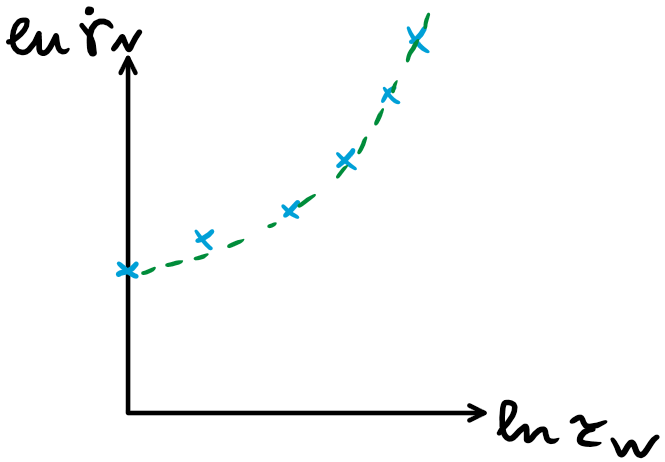
\includegraphics[width = 0.7\textwidth]{gfx/CorrezioneDoppioLog}
\caption{Descrizione del fattore di Rabinowitch ottenuto sperimentalmente}
\label{fig:CorrezioneDoppioLog}
\end{figure}

\subsection{Correzione di Bagley}
COme già visto, l'equazione dello sforzo di taglio è la seguente:
\begin{equation}
\tau_W = \frac{\Delta P R}{2L} \quad \tau_W =\frac{PR}{2L}
\end{equation}
Dove con $\Delta P$ sono le perdite di carico totali relative al processo di estrusione.
Alla base di questa equazione, c'è l'ipotesi di poter trascurare i seguenti fenomeni:
\begin{itemize}
\item La possibilità di un non perfetto accoppiamento tra pistone matrice.
\item Gli attriti derivanti dal moto nella camera.
\item Le perdite di carico in ingresso, dovute al riarrangiamento del profilo di velocità che si ha all'entrata dell'ugello.
Tale riarrangiamento è dovuto al restringimento del filetto fluido delle dimensioni della matrice a quelle del capillare.
\item Altro contributo a tali perdite è il gradiente di pressione maggiore che si ha nella prima parte del capillare, derivante da un flusso non ancora perfettamente sviluppato.
\end{itemize}

Mentre i primi tre contributi sono senz'altro trascurabili, altrettanto non si può dire per gli ultimi due. Per tener conto di questi effetti, viene introdotta la correzione di \eng{Bagley}.
Si tratta di valutare le perdite di carico totali per ugelli con diversi rapporti $L/R$ ad un determinato valore di gradiente di velocità.
Riportando su un grafico \ref{fig:Bagley} i valori trovati, si estrapola il valore delle perdite di carico per $L/R = 0$%
\footnote{Ovvero il punto di incontro della retta con l'asse delle ordinate},
assumendo che questo coincida con la somma delle perdite di carico in entrata ed in uscita a quel determinato gradiente di velocità.
L'operazione viene poi ripetuta per ogni gradiente di velocità, ottenendo così un vettore di perdite di carico.

\begin{figure}
\centering
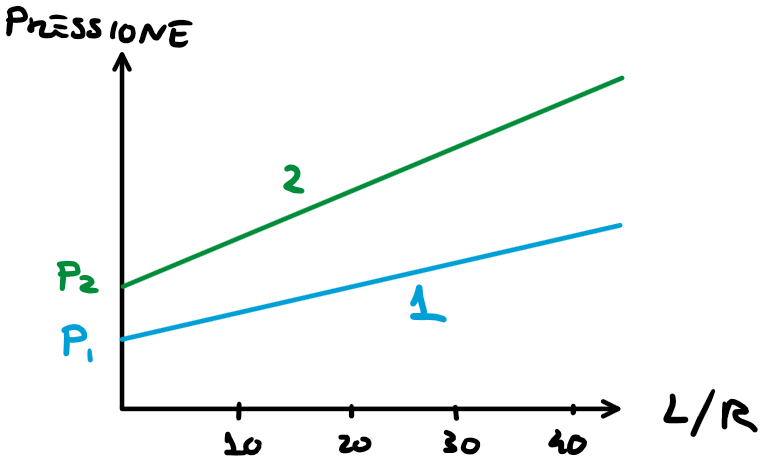
\includegraphics[width = 0.7\textwidth]{gfx/Bagley}
\caption{Rette di Bagley}
\label{fig:Bagley}
\end{figure}

Allora il valore dello sforzo di taglio:
\begin{equation}
\tau_W = \frac{PR}{2(L + L^*)} = \frac{PR}{2(L + eR)}
\end{equation}
Le perdite saranno:
\begin{equation}
P = \frac{\tau_W 2(L + eR)}{R}
\end{equation}
Allora ne risulta
\begin{equation}
\dot{\gamma}_N = \frac{4Q}{\pi R^3}
\end{equation}
Ipotizzando  che $Q$ e $R$ siano costanti allora anche $\dot{\gamma}_N$ sarà costante.
Dato che $\tau_W = \eta \cdot \dot{\gamma}_N$, allora anche $\tau_W$ sarà costante.

% ********************************************************************
% Backmatter
%*******************************************************
\appendix
%\renewcommand{\thechapter}{\alph{chapter}}
\cleardoublepage
\part{Appendix}
%************************************************
\chapter{Esercizi Peso molecolare}\label{chp:EsercizioPM}
%************************************************
Data la distribuzione delle frazioni molecolari, tabella \ref{tab:EsercizioPM}: 
\begin{enumerate}
\item calcolare il peso molecolare medio e il peso molecolare ponderale.
\item Se il peso molecolare del monomero è $56$, calcolare il grado di polimerizzazione .
\end{enumerate}

\begin{table}
\caption{Distribuzione della media dei pesi molecolari delle frazioni polimeriche}
\label{tab:EsercizioPM}
$
\begin{array}{cc}
\toprule
M_i & \phi_i\\
\unit{\kg/\mol} & \\
\midrule
14 & 0.05\\
26 & 0.15\\
38 & 0.21\\
50 & 0.28\\
62 & 0.15\\
74 & 0.10\\
86 & 0.03\\
\bottomrule
\end{array}
$
\end{table}
Allora:
\begin{equation}
\bar{M}_n = \sum_i{\phi_iM_i} = 47.9\unit{\kg/\mol}
\end{equation}
Per calcolare la frazione ponderale a partire dalla frazione molecolare
\begin{equation}
\begin{split}
W_j &= N_j M_j\\
\frac{\psi_j}{\phi_j} &= \frac{\frac{W_j}{W}}{\frac{N_j}{N}} = \frac{\frac{W_j}{N_j}}{\frac{W}{N}}\\
&=\frac{M_j}{\bar{M}_n}
\end{split}
\end{equation}
Da cui:
\begin{equation}
\begin{split}
\psi_i &= \frac{\phi_iM_i}{\bar{M}_n}\\
\bar{M}_w &= \sum_i{\psi_iM_i} = 53.4\unit{\kg/\mol}
\end{split}
\end{equation}
Conviene calcolare \ac{IPD} per arrivare al grado di polimerizzazione:
\begin{equation}
IPD = \frac{\bar{M}_w}{\bar{M}_n} = 1.1\,\textup{monodisperso}
\end{equation}
In fine:
\begin{equation}
\begin{split}
\bar{M}_n &= \frac{W}{N} = \frac{W}{\sum_j{N_j}} = \frac{W}{\sum_j{\frac{W_j}{M_j}}} =\\
&= \frac{1}{\sum_j{\frac{W_j}{W}\frac{1}{M_j}}} = \frac{1}{\sum_j{\frac{\psi_j}{M_j}}}\\
\frac{1}{\bar{M}_n} &= \sum_j{\frac{\psi_j}{M_j}}
\end{split}
\end{equation}
\begin{equation}
\bar{n} = \frac{\bar{M}_n}{PM_{\textup{monomero}}} = \frac{53400\unit{\g/\mol}}{56\unit{\g/\mol}} = 851
\end{equation}


%************************************************
\chapter{Esercizi sulla viscoelasticità lineare}\label{chp:VisElastLineare}
%************************************************
\section{Esercizio}
$E = E(t)$ come in figura \ref{fig:Esercizio1} e storia di deformazione.
Se ne calcoli lo sforzo.

\begin{figure}
\centering
\subfloat[][\emph{Andamento rilassamento}\label{fig:Esercizio1_E}]
{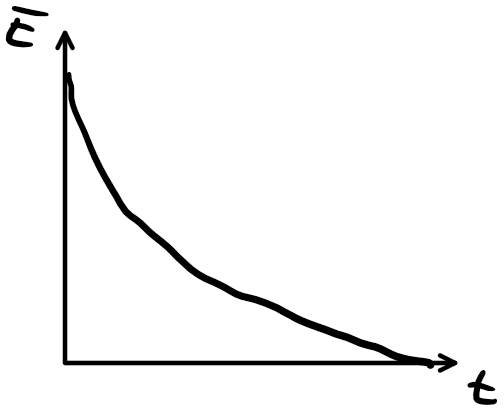
\includegraphics[width = 0.4\textwidth]{gfx/Esercizio1_E}}\quad
\subfloat[][\emph{Storia deformazione}\label{fig:Esercizio1_eps}]
{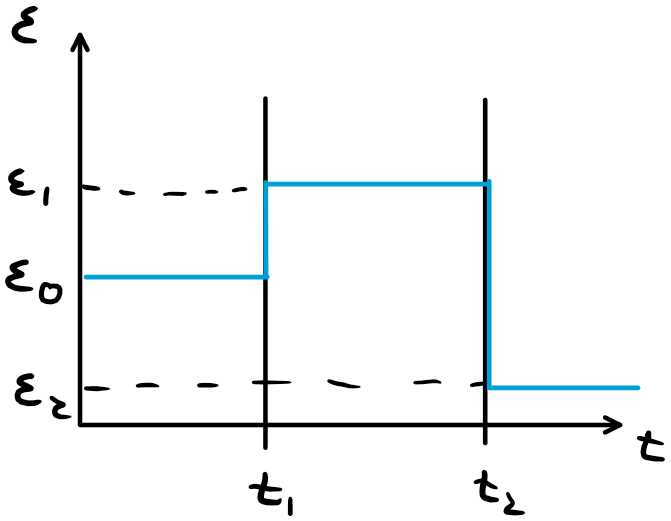
\includegraphics[width = 0.4\textwidth]{gfx/Esercizio1_eps}}
\caption{Esercizio 1 viscoelasticità lineare}
\label{fig:Esercizio1}
\end{figure}

Si nota che la funzione $\epsilon(t)$ è lineare a tratti, per cui suddivideremo in intervalli dove è lineare.
\begin{description}
\item[$0 < t < t_1$] allora:
\begin{equation}
\begin{cases}
\epsilon(t) &= \epsilon_0 \quad \forall t \in [0;t_1)\\
\sigma(t) &= \epsilon_0 E(t)
\end{cases}
\end{equation}
\item[$t_1 < t < t_2$]
In questo caso bisogna considerare che c'è il rilassamento della deformazione precedente più lo sforzo della nuova deformazione.
Da cui:
\begin{equation}
\sigma = \epsilon_0E(t) + (\epsilon_1 - \epsilon_0)E(t) = [\epsilon_0 + \epsilon_1 - \epsilon_0]E(t)???
\end{equation}
Non è corretto infatti è erronea la sovrapposizione degli effetti:
\begin{equation}
\sigma = \epsilon_0E(t) + (\epsilon_1 - \epsilon_0)E(t-t_1)
\end{equation}
\item[$t>t_2$] per lo stesso ragionamento precedente:
\begin{equation}
\sigma = \epsilon_0E(t) + (\epsilon_1 - \epsilon_0)E(t-t_1) + (\epsilon_2 - \epsilon_1)E(t - t_2)
\end{equation}
\end{description}

\begin{figure}
\centering
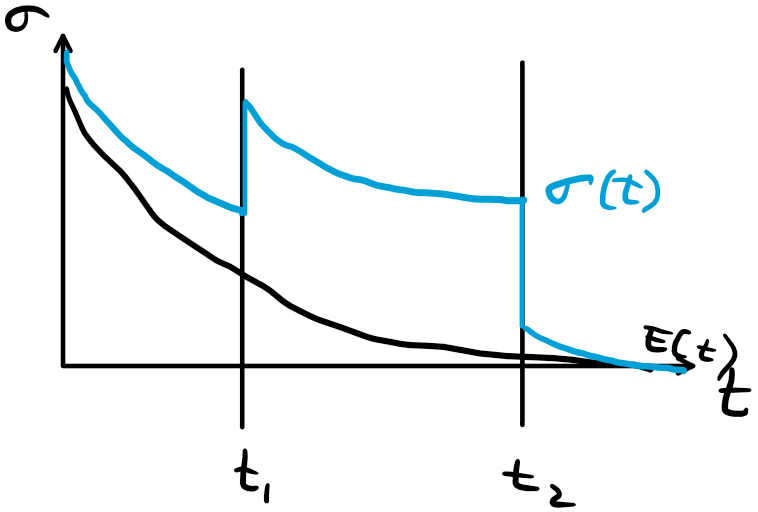
\includegraphics[width = \textwidth]{gfx/Risultato1}
\caption{Risultato dell'esercizio 1}
\label{fig:Risultato1}
\end{figure}

\section{Esercizio}
Confronto di due storie di deformazione differenti:

\begin{figure}
\centering
\subfloat[][\emph{Andamento rilassamento}\label{fig:Esercizio2_E}]
{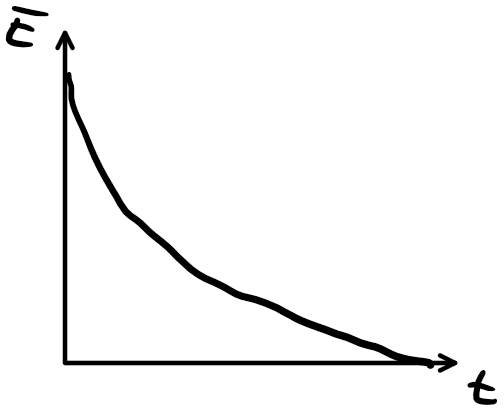
\includegraphics[width = 0.4\textwidth]{gfx/Esercizio1_E}}\quad
\subfloat[][\emph{Storie di deformazione}\label{fig:Esercizio2_eps}]
{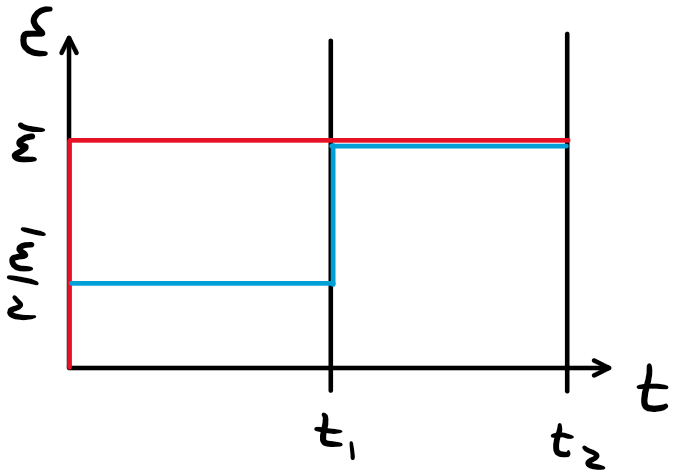
\includegraphics[width = 0.4\textwidth]{gfx/Esercizio2_eps}}
\caption{Andamenti per il confronto delle due storie di deformazione}
\label{fig:Esercizio2}
\end{figure}

\paragraph{Soluzione}
allora:
\begin{description}
\item[Storia rossa \ref{fig:Esercizio2_eps}] $\epsilon = \bar{\epsilon} \Rightarrow \sigma(t_2) = \bar{\epsilon}E(t_2)$
\item[Storia azzurra \ref{fig:Esercizio2_eps}] in questo caso:
\begin{equation}
\sigma(t_2) =%
\begin{cases}
\frac{\bar{\epsilon}}{2} &0<t<t_1\\
\bar{\epsilon} &t_1<t<t_2
\end{cases}
\end{equation}
\end{description}
Ne caso della seconda storia, osserviamo l'andamento dello sforzo:
\begin{equation}
\sigma(t_2) = \frac{\bar{\epsilon}}{2}E(t_2) + [\bar{\epsilon} - \frac{\bar{\epsilon}}{2}]E(t_2 - t_1)
\end{equation}
Ne risulta che siccome $t_2 > t_2-t_1$ e siccome la deformazione è una funzione decrescente: $E(t_2)< E(t_2-t_1)$.
Dunque lo sforzo conseguente la storia rossa è minore di quella azzurra.

\section{Esercizio}
Considerando un solido a tre parametri come in figura \ref{fig:Esercizio3_Fluido}.
Con le differenti storie di deformazione \ref{fig:Esercizio3_eps1} e \ref{fig:Esercizio3_eps2}.

\begin{figure}
\centering
\subfloat[][\emph{Solido a tre parametri}\label{fig:Esercizio3_Fluido}]
{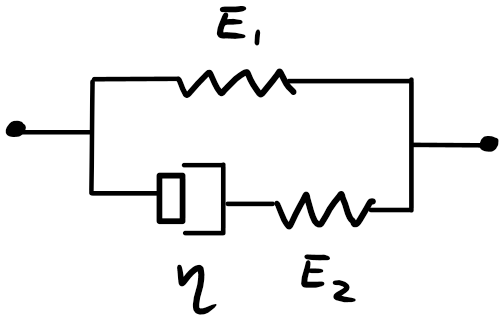
\includegraphics[width = 0.5\textwidth]{gfx/Esercizio3_Fluido}}\\
\subfloat[][\emph{Prima storia di deformazione}\label{fig:Esercizio3_eps1}]
{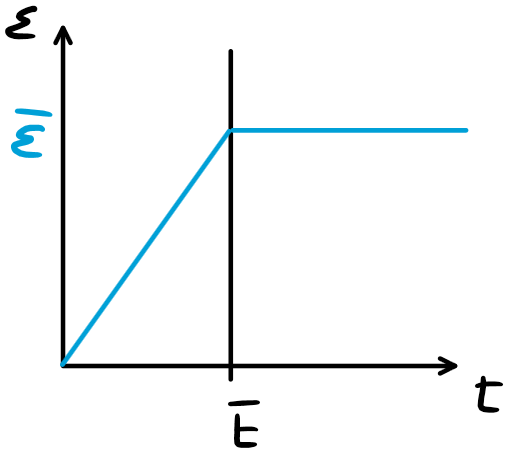
\includegraphics[width = 0.4\textwidth]{gfx/Esercizio3_eps1}}\quad
\subfloat[][\emph{Seconda storia di deformazione}\label{fig:Esercizio3_eps2}]
{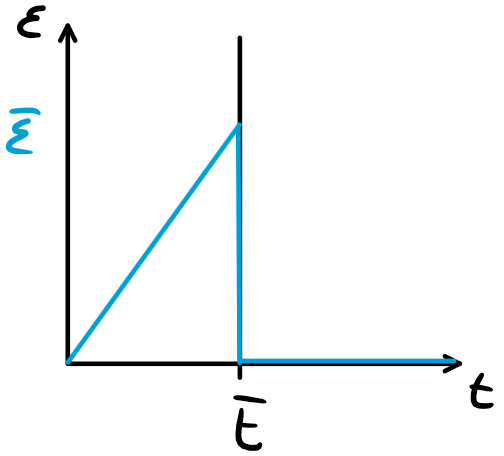
\includegraphics[width = 0.4\textwidth]{gfx/Esercizio3_eps2}}
\caption{Esercizio 3}
\label{fig:Esercizio3}
\end{figure}

\paragraph{Soluzione}
Allora:
\begin{equation}
\begin{split}
\dot{\epsilon} &= \dot{\epsilon}_1 + \dot{\epsilon}_3 = \frac{\dot{\sigma}_2}{E_2} + \frac{\dot{\sigma}_3}{\eta_3}\\
&=\frac{\dot{\sigma}}{E_2} - \frac{\dot{\sigma}_1}{E_2} + \frac{\sigma}{\eta_3} - \frac{\sigma_1}{\eta_3}\\
&= \frac{\dot{\sigma}}{E_2} - \frac{E_1\dot{\epsilon}}{E_2} + \frac{\sigma}{\eta_3} - \frac{\sigma_1\epsilon}{\eta_3}\\
\frac{\dot{\sigma}}{E_2} &+\frac{\sigma}{\eta_3} = \left(1 + \frac{E_1}{E_2}\right)\dot{\epsilon} + \frac{E_1}{\eta_3}\epsilon
\end{split}
\end{equation}

Imponiamo la storia di deformazione \ref{fig:Esercizio3_eps1}:
\begin{equation}
\epsilon(t) = \frac{\bar{\epsilon}}{\bar{t}}t \qquad \dot{\epsilon} = \frac{\bar{\epsilon}}{\bar{t}}
\end{equation}
Applicandolo, all'equazione differenziale:
\begin{equation}
\begin{split}
\frac{\dot{\sigma}}{E_2}&+\frac{\sigma}{\eta_3} = \left(1+\frac{E_1}{E_2}\right)\frac{\bar{\epsilon}}{\bar{t}} + \frac{E_1}{\eta_3}\frac{\bar{\epsilon}}{\bar{t}}t\\
\sigma(t) &= \sigma_h + \sigma_p =%
\begin{cases}
\sigma_h(t) = C e^{-\frac{t}{\tau_r}} \quad \tau_r = \frac{\eta_3}{E_2}\\
\sigma_p(t) = A+Bt
\end{cases}
\end{split}
\end{equation}
Affinché sia soluzione deve valere che l'equazione abbia soluzione nelle componenti omogenee e particolare.
Dunque sostituiamo a $\sigma$, $\sigma_p$.
\begin{equation}
\begin{split}
\frac{B}{E_2} &+ \frac{A}{\eta_3} + \frac{B}{\eta_3}t = \left(1+\frac{E_1}{E_2}\right)\frac{\bar{\epsilon}}{\bar{t}} + \frac{E_1}{\eta_3}\frac{\bar{\epsilon}}{\bar{t}}t\\
&\begin{cases}
B = E_1\frac{\bar{\epsilon}}{\bar{t}}\\
A = \eta_3 \frac{\epsilon}{\bar{t}}
\end{cases}\\
\sigma(t) &= \eta_3 \frac{\bar{\epsilon}}{\bar{t}} + E_1\frac{\bar{\epsilon}}{\bar{t}}t + C e^{-\frac{t}{\tau_r}}\\
t &= 0 \rightarrow 0 = \eta_3 \frac{\bar{\epsilon}}{\bar{t}} + C \Rightarrow C = -\eta_3\frac{\bar{\epsilon}}{\bar{t}}\\
\sigma(t) &= E_1\frac{\bar{\epsilon}}{\bar{t}}t + \eta_3\frac{\bar{\epsilon}}{\bar{t}}\left(1 - e^{-\frac{t}{\tau_r}}\right) 
\end{split}
\end{equation}

Il secondo tratto della storia di deformazione è costante, per cui vale:
\begin{equation}
\frac{\dot{\sigma}}{E_2} + \frac{\sigma}{\eta_3} = \frac{E_1}{\eta_3}\bar{\epsilon}
\end{equation}
Allora:
\begin{equation}
\sigma(t) = C e^{-\frac{t}{\tau_r}} + E_1\bar{\epsilon}
\end{equation}
In $t = \bar{t}$:
\begin{equation}
\begin{split}
\sigma(t) &= E_1\bar{\epsilon} + \eta_3\frac{\bar{\epsilon}}{\bar{t}}\left(1 - e^{-\frac{\bar{t}}{\tau_r}}\right)\\
\sigma(t) &= E_1\bar{\epsilon} + \eta_3\frac{\bar{\epsilon}}{\bar{t}}\left(e^{-\frac{t-\bar{t}}{\tau_r}} - e^{-\frac{t}{\tau_r}}\right)
\end{split}
\end{equation}
La soluzione dovrebbe essere quella in figura \ref{fig:Soluzione3}.
Per la storia di deformazione \ref{fig:Esercizio3_eps2}
la soluzione sta nel considerare la discontinuità come $-(E_1 - E_2)\bar{\epsilon}$

\begin{figure}
\centering
\includegraphics[width = 0.5\textwidth]{gfx/Soluzione3}
\caption{Soluzione dell'esercizio}
\label{fig:Soluzione3}
\end{figure}
%************************************************
\chapter{Tavola periodica}\label{chp:Tavolaperiodica}
%************************************************
\newpage
\includegraphics[scale = 1, angle = 90]{gfx/Periodic_table2017}
%********************************************************************
% Other Stuff in the Back
%*******************************************************
\cleardoublepage%********************************************************************
% Bibliography
%*******************************************************
% work-around to have small caps also here in the headline
\manualmark
\markboth{\spacedlowsmallcaps{\bibname}}{\spacedlowsmallcaps{\bibname}} % work-around to have small caps also
%\phantomsection 
\refstepcounter{dummy}
\addtocontents{toc}{\protect\vspace{\beforebibskip}} % to have the bib a bit from the rest in the toc
\addcontentsline{toc}{chapter}{\tocEntry{\bibname}}
\label{app:bibliography}
\printbibliography

\cleardoublepage%*******************************************************
% Declaration
%*******************************************************
\refstepcounter{dummy}
\pdfbookmark[0]{Declaration}{declaration}
\chapter*{Declaration}
\thispagestyle{empty}
Put your declaration here.
\bigskip
 
\noindent\textit{\myLocation, \myTime}

\smallskip

\begin{flushright}
    \begin{tabular}{m{5cm}}
        \\ \hline
        \centering\myName \\
    \end{tabular}
\end{flushright}

\cleardoublepage\pagestyle{empty}

\hfill

\vfill


\pdfbookmark[0]{Colophon}{colophon}
\section*{Colophon}
This document was typeset using the typographical look-and-feel \texttt{classicthesis} developed by Andr\'e Miede. 
The style was inspired by Robert Bringhurst's seminal book on typography ``\emph{The Elements of Typographic Style}''. 
\texttt{classicthesis} is available for both \LaTeX\ and \mLyX: 
\begin{center}
\url{https://bitbucket.org/amiede/classicthesis/}
\end{center}
Happy users of \texttt{classicthesis} usually send a real postcard to the author, a collection of postcards received so far is featured here: 
\begin{center}
\url{http://postcards.miede.de/}
\end{center}
 
\bigskip

\noindent\finalVersionString

%Hermann Zapf's \emph{Palatino} and \emph{Euler} type faces (Type~1 PostScript fonts \emph{URW
%Palladio L} and \emph{FPL}) are used. The ``typewriter'' text is typeset in \emph{Bera Mono}, 
%originally developed by Bitstream, Inc. as ``Bitstream Vera''. (Type~1 PostScript fonts were made 
%available by Malte Rosenau and
%Ulrich Dirr.)

%\paragraph{note:} The custom size of the textblock was calculated
%using the directions given by Mr. Bringhurst (pages 26--29 and
%175/176). 10~pt Palatino needs  133.21~pt for the string
%``abcdefghijklmnopqrstuvwxyz''. This yields a good line length between
%24--26~pc (288--312~pt). Using a ``\emph{double square textblock}''
%with a 1:2 ratio this results in a textblock of 312:624~pt (which
%includes the headline in this design). A good alternative would be the
%``\emph{golden section textblock}'' with a ratio of 1:1.62, here
%312:505.44~pt. For comparison, \texttt{DIV9} of the \texttt{typearea}
%package results in a line length of 389~pt (32.4~pc), which is by far
%too long. However, this information will only be of interest for
%hardcore pseudo-typographers like me.%
%
%To make your own calculations, use the following commands and look up
%the corresponding lengths in the book:
%\begin{verbatim}
%    \settowidth{\abcd}{abcdefghijklmnopqrstuvwxyz}
%    \the\abcd\ % prints the value of the length
%\end{verbatim}
%Please see the file \texttt{classicthesis.sty} for some precalculated 
%values for Palatino and Minion.
%
%    \settowidth{\abcd}{abcdefghijklmnopqrstuvwxyz}
%    \the\abcd\ % prints the value of the length





% ********************************************************************
% Game Over: Restore, Restart, or Quit?
%*******************************************************
\end{document}
% ********************************************************************
